
\chapter{\label{chapter4_MA4}MLL-AF4 and RUNX1 driven regulatory networks in \textit{MLL}r leukaemia}
\chaptermark{Chapter 4 - MLL-AF4 GRN}

\begingroup
\raggedright
\minitoc
\endgroup

\clearpage % Keep contents seperate page

% Put declaration here?!

\section{Introduction and aims}

In chapter \ref{chapter3_EHT} I established a GRN model of mouse EHT. This is a normal haematopoietic process, describing the differentiation of aortic endothelium towards HSCs. I focused the analysis of this model on the activity of Runx1, and I used an analytical approach to predict possible TF cooperation. For this chapter, I asked how abnormal haematopoiesis may be regulated. MLL-AF4 leukaemias are considered a transcriptional disease, as the translocation event can be sufficient on its own for leukaemogenesis, with few or no cooperative mutations \citep{bardini_dna_2010, bardini_implementation_2011, the_cancer_genome_atlas_research_network_genomic_2013, andersson_landscape_2015}. As described in section \ref{ch1:mll-af4-function}, MLL-AF4 binds to gene promoters and drives transcription through the recruitment of a large transcription elongation complex \citep{ballabio_molecular_2012, slany_mll_2020}. This makes \textit{MLL}r leukaemias particularly suited for analysis using GRN methods, which rely on transcriptional data. Additionally, the MLL-AF4 fusion protein maintains overexpressed \textit{RUNX1} expression \citep{wilkinson_runx1_2013}, which allows for the study of dysregulated RUNX1 activity in a leukaemic network context.

\begin{figure}[!t]
    \centering
    %\includegraphics[width=\textwidth,height=\textheight,keepaspectratio]{figures/chapter4/ch1_grn-justification.png}
    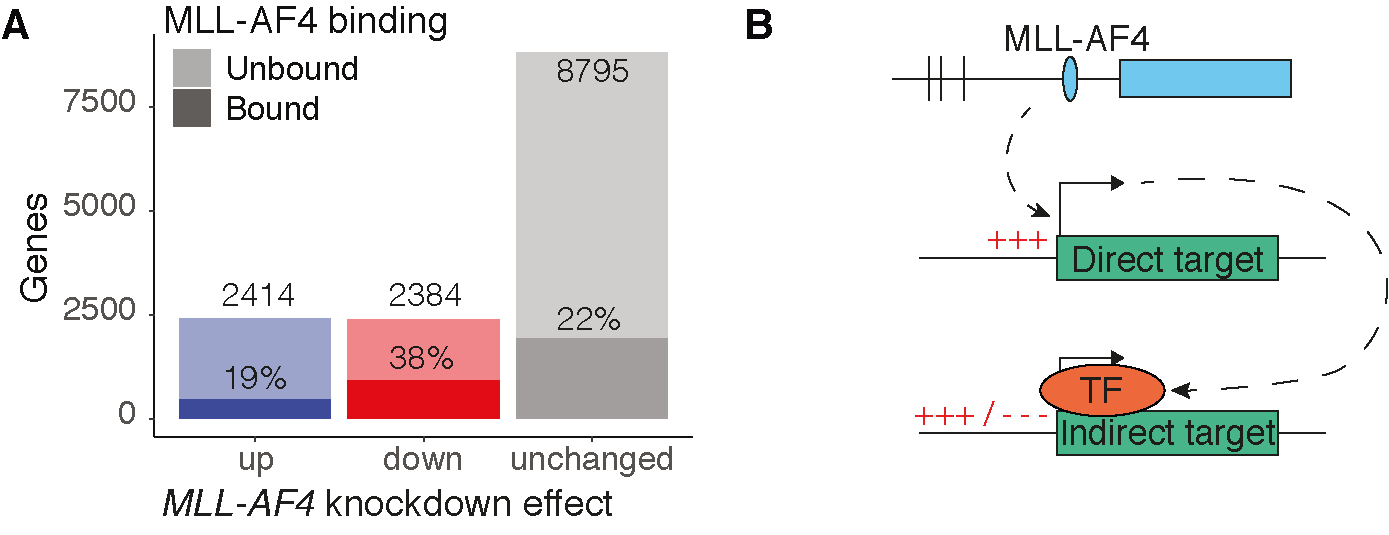
\includegraphics{figures/chapter4/ch4_grn-justification.png}
    \caption[{MLL-AF4 regulation cannot be explained by direct binding alone.}]
    {\textbf{MLL-AF4 regulation cannot be explained by direct binding alone.} 
    \textbf{(A)} Number of DEGs after 96 h \textit{MLL-AF4} KD in SEM cells (\textit{n} = 3). Shaded bar represents proportion of DEGs bound by MLL-AF4 (ChIP-seq). 
    \textbf{(B)} Schematic illustrating hypothesis, where MLL-AF4 regulates TFs, which then regulate additional targets, resulting in indirect downstream regulation. 
    \textit{Analysis in A first performed by R. Thorne. Adapted from \cite{harman_kmt2a-aff1_2021}.}
    }
    \label{fig:ch4_GRN_just}
\end{figure}

As the MLL-AF4 complex directly promotes transcription \citep{ballabio_molecular_2012, biswas_function_2011, kerry_mll-af4_2017, mueller_role_2007, yokoyama_higher-order_2010, lin_aff4_2010, okuda_af4_2015} and is the main driver of leukaemogenesis, it is expected that \textit{MLL-AF4} KD would lead to downregulation of gene expression, with affected genes bound by MLL-AF4 protein. Previous analysis by R. Thorne (Milne lab) of nascent RNA-seq following \textit{MLL-AF4} KD \citep{godfrey_mll-af4_2017} in the SEM cell line (B-ALL MLL-AF4, \cite{greil_acute_1994}) established that this is not true. Only 28\% of \textit{MLL-AF4} KD sensitive genes were bound by MLL-AF4, and both up- and downregulation was observed (Fig. \ref{fig:ch4_GRN_just}A, \cite{harman_kmt2a-aff1_2021}). To explain this discrepancy, I hypothesised these non-bound genes are indirectly regulated via intermediate TFs that are overactivated as a consequence of MLL-AF4 activity (Fig. \ref{fig:ch4_GRN_just}B). As TFs often do not act in isolation \citep{morgunova_structural_2017, spitz_transcription_2012}, it is important to address the possibility that MLL-AF4 may function in combination with other TFs to regulate gene targets, and thus understand the full regulatory scope of MLL-AF4. As such, a GRN model of MLL-AF4 leukaemia was established to decode complex combinatorial signals and organise direct and indirect regulatory logic, by isolating common network motifs such as FFLs and TF cascades. 

\noindent
\textbf{Aims} 

\vspace*{-5mm}
\begin{enumerate}
    \item To determine if MLL-AF4 controls a wider transcriptional network through TF activation. 
    \item To determine whether the MLL-AF4 GRN can be used to identify novel biology of MLL-AF4 leukaemias.
    \item To investigate the TF cooperativity between MLL-AF4, RUNX1, and its target TFs.
\end{enumerate}

\vspace*{-5mm}
By constructing a GRN model of MLL-AF4 leukaemia, the regulatory logic downstream of MLL-AF4 can be explored. This allows us to address the hypothesis that MLL-AF4 regulates targets indirectly via intermediate TFs. It is important to determine whether the GRN can describe the biology of leukaemia, and its relevance to real-world patient samples. As in chapter 3, a dissection of how MLL-AF4 and RUNX1 cooperate with other TFs will explore into a less studied area of gene regulation, and could offer insight into the role of intermediate TFs in MLL-AF4 leukaemia.

\clearpage


\section{\label{ch4:grn}Generating and characterising a GRN model of MLL-AF4 driven leukaemia}

To determine whether MLL-AF4 was able to control the expression of a wider transcriptional network by activating TFs, I sought to integrate nascent RNA-seq and ChIP-seq datasets generated in SEM cells (B-ALL MLL-AF4) to establish a GRN model. MLL-AF4 DNA binding is not well predicted through specific motifs. The part of MLL-AF4 that contacts DNA is the CxxC domain which confers binding preference for uCpGs \citep{birke_mt_2002}. However, MLL-AF4 only binds to a subset uCpGs and it is unknown what guides this preference \citep{kerry_mll-af4_2017}. As such, MLL-AF4 ChIP-seq \citep{kerry_mll-af4_2017} was used as evidence for direct binding, while nascent RNA-seq following 96 hours' \textit{MLL-AF4} KD \citep{kerry_mll-af4_2017} was used to identify the regulatory scope of MLL-AF4, including indirect targets. 

\begin{figure}[htbp]
    \centering
    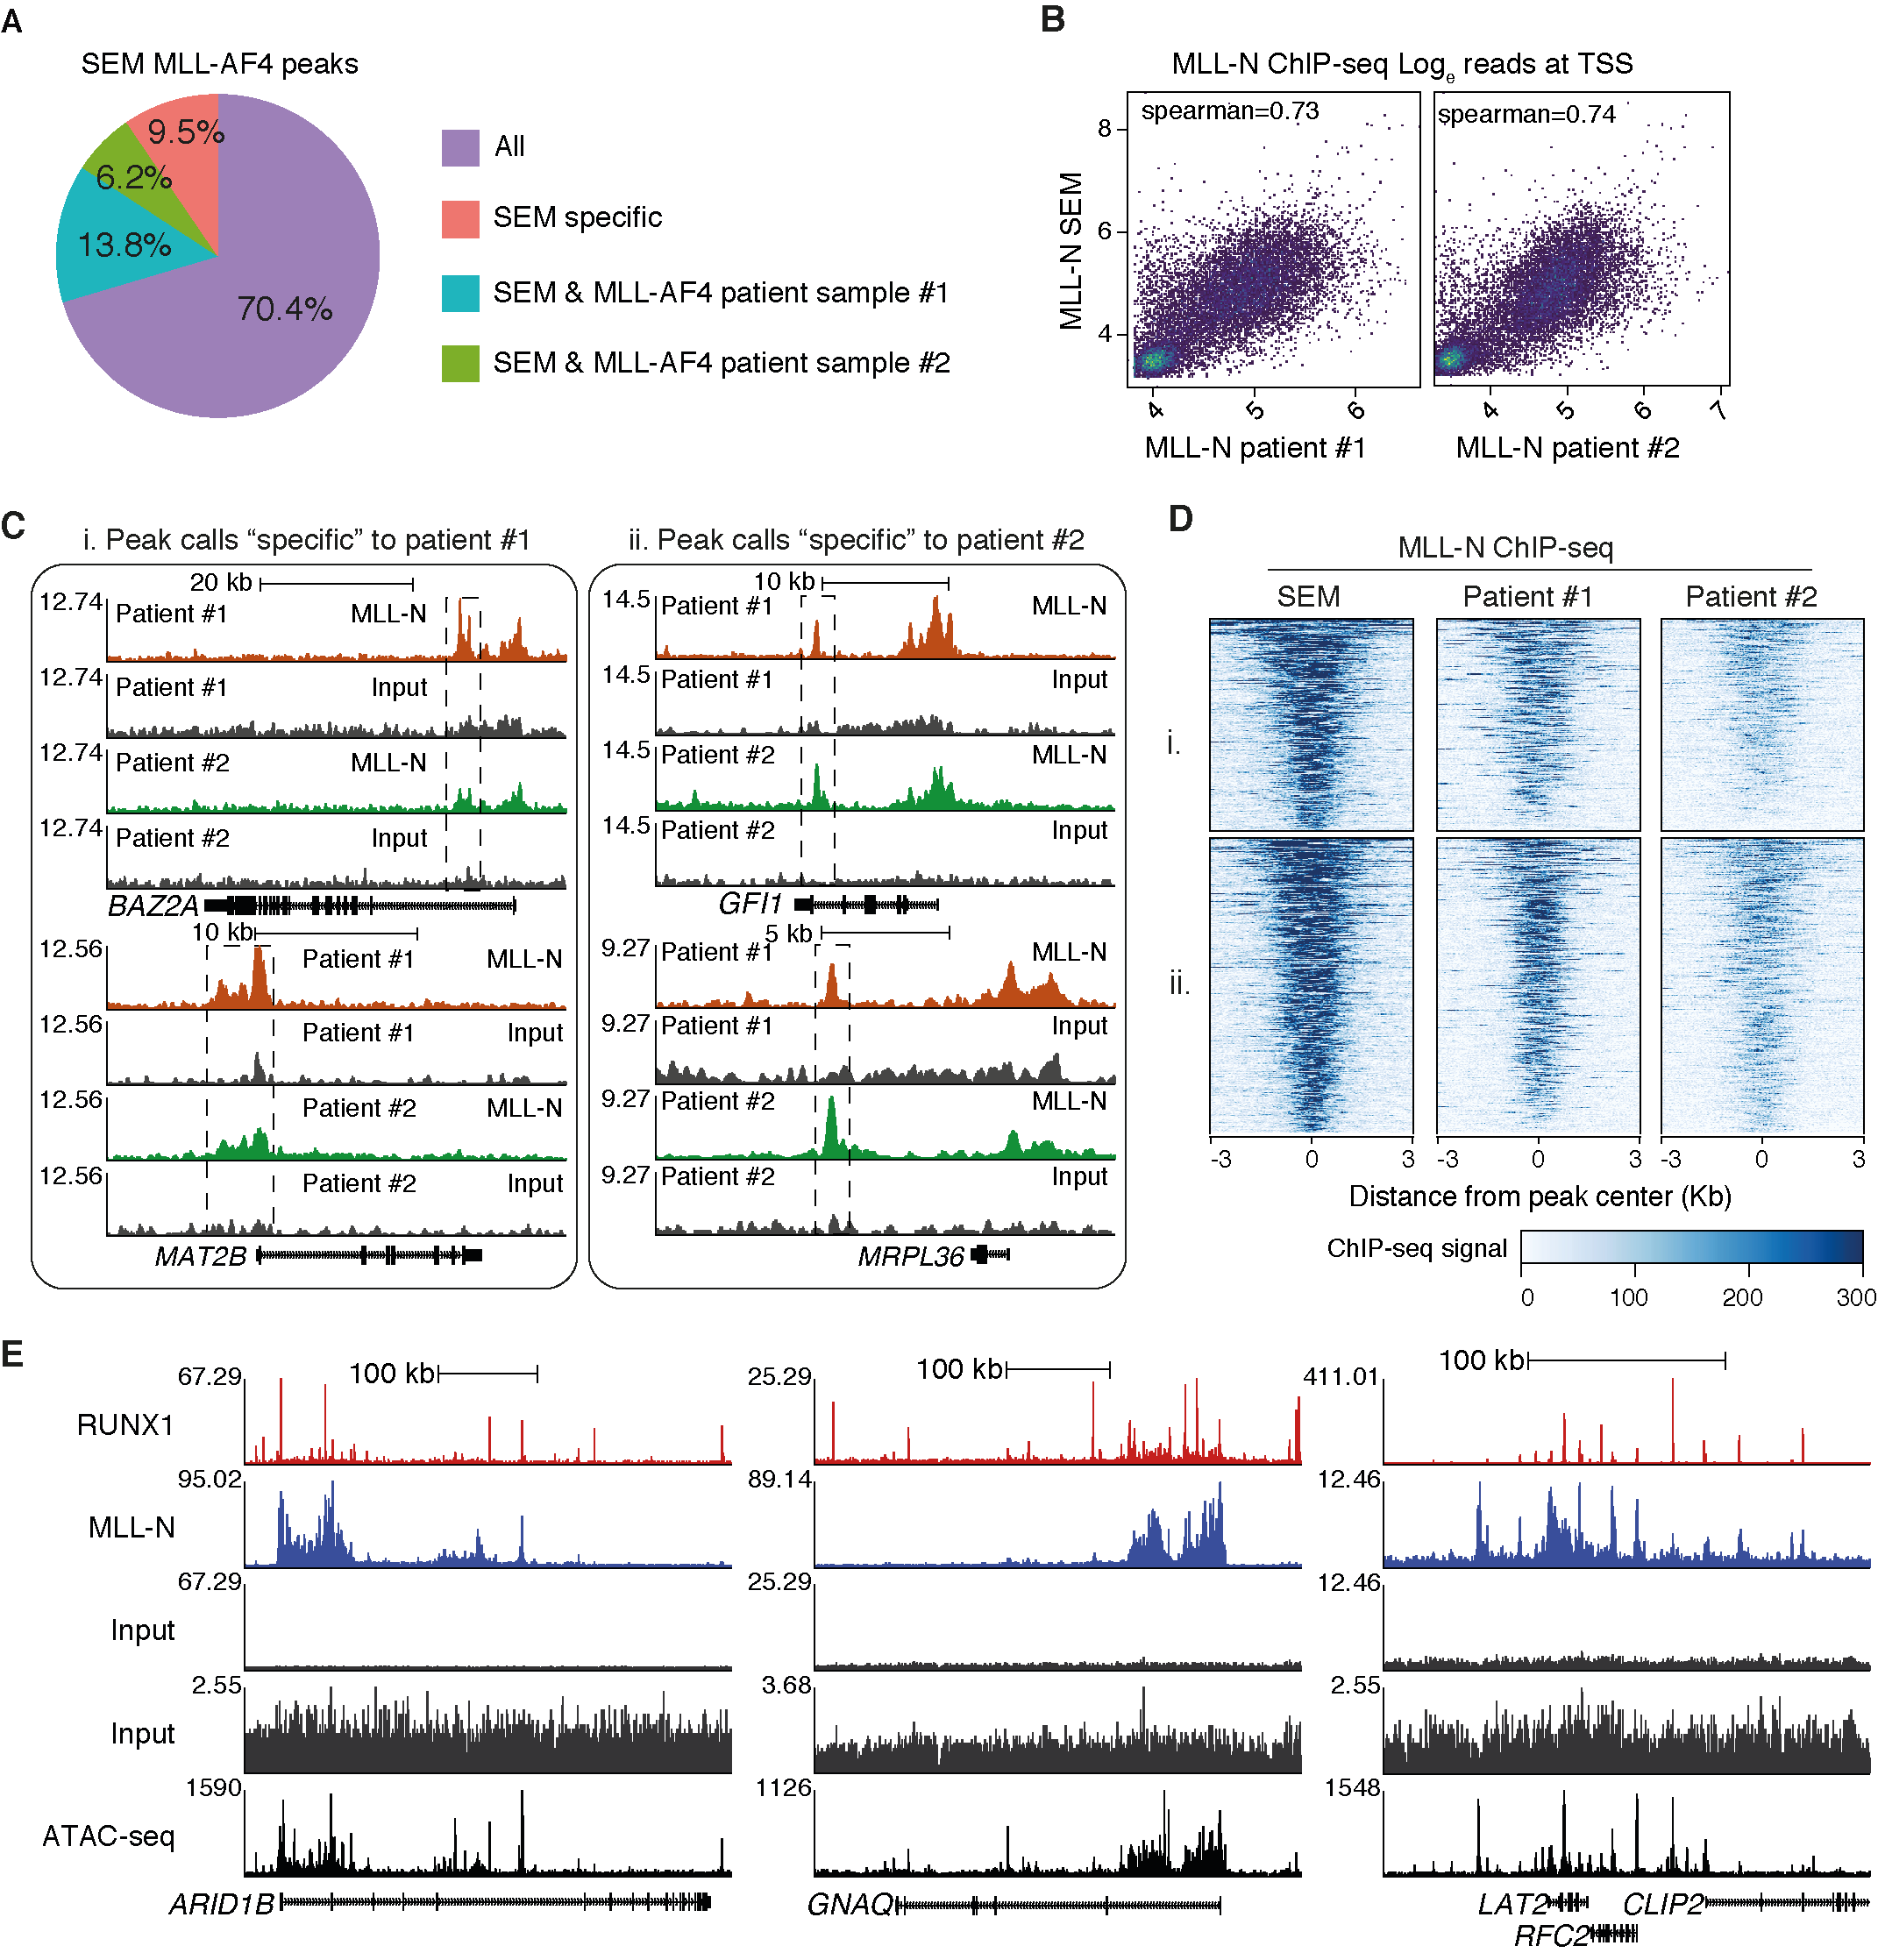
\includegraphics[width=\textwidth,keepaspectratio]{figures/chapter4/ch4_peak-qc.png}
    %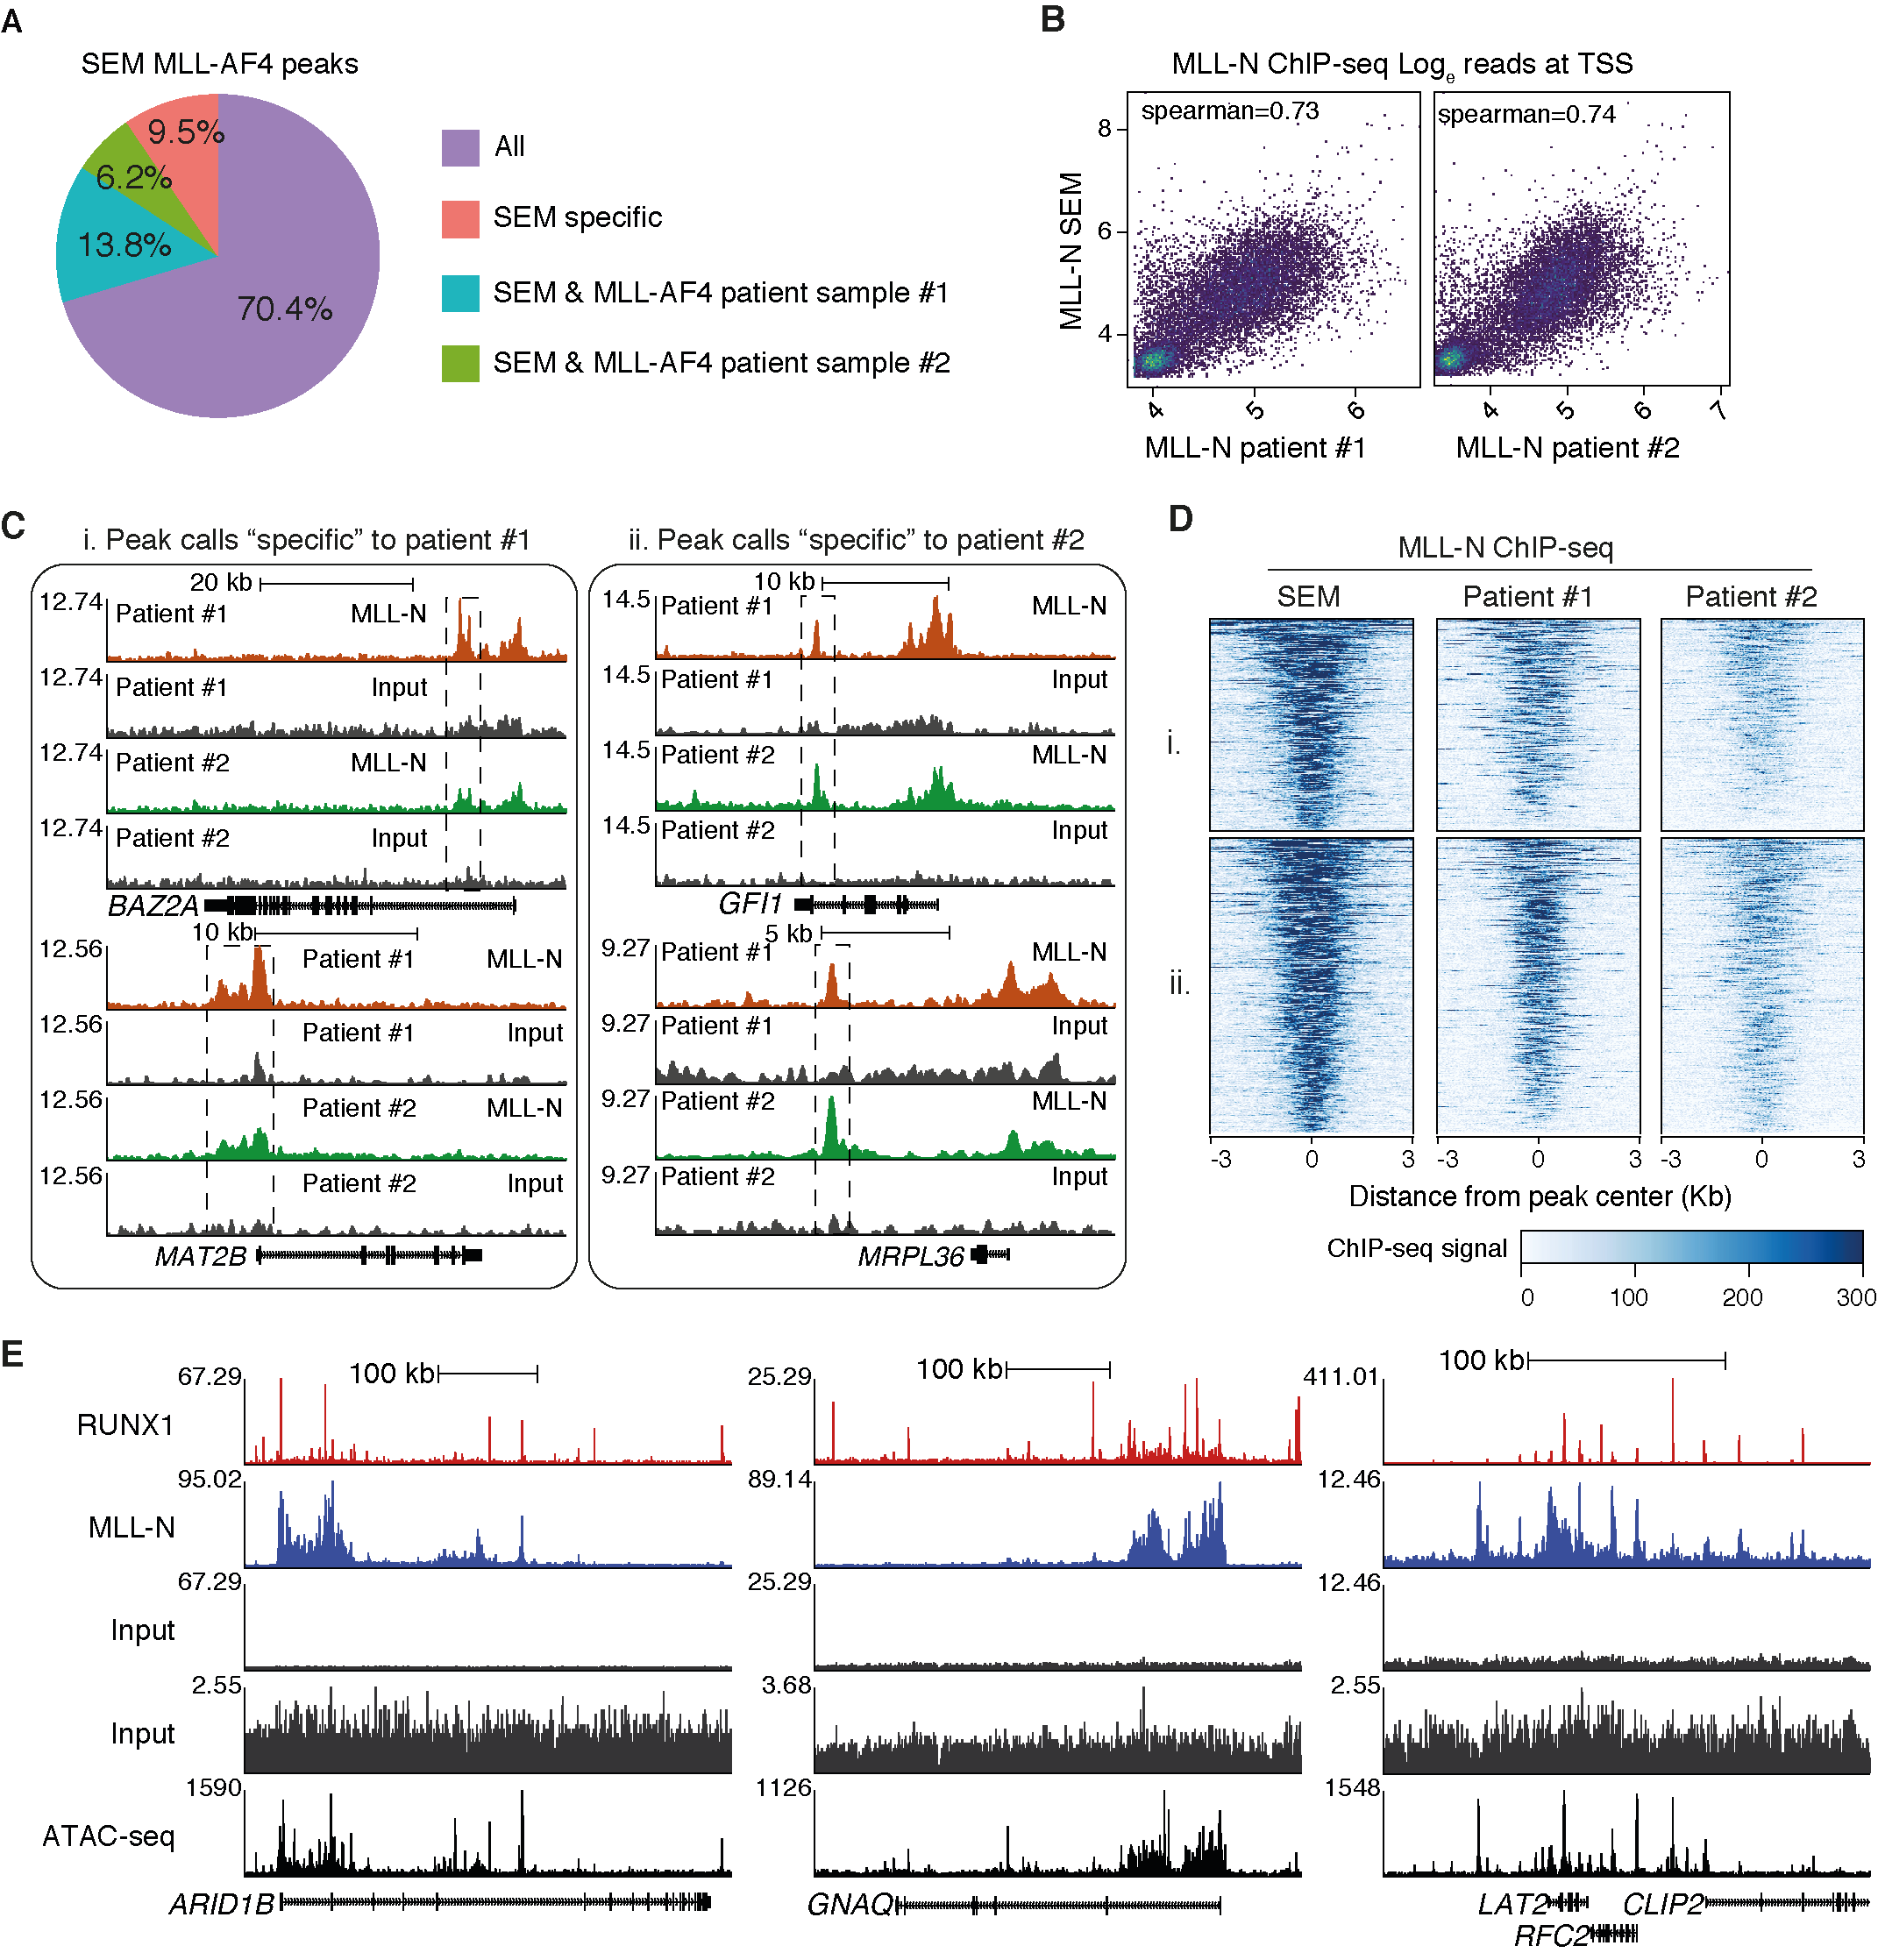
\includegraphics{figures/chapter4/ch4_peak-qc.png}
    \caption[{ChIP-seq data is of sufficient quality for GRN analysis.}]
    {\textbf{ChIP-seq data is of sufficient quality for GRN analysis.} 
    \textbf{(A)} Proportion of MLL-AF4 peaks in SEM cells that overlap with MLL-AF4 peaks in patient samples. 
    \textbf{(B)} Comparison of Log\textsubscript{e} MLL-N reads at gene promoters in SEM cells and patient samples. 
    \textbf{(C)} ChIP-seq tracks for MLL-N and input chromatin. Loci are MLL-AF4-bound genes unique to patient \#1 (i) or patient \#2 (ii), as defined in A. Boxed regions indicate peak calls of interest. 
    \textbf{(D)} ChIP-seq heatmaps for MLL-N. Loci are SEM MLL-N peaks with peak calls unique to patient \#1 (i) or patient \#2 (ii). 
    \textbf{(E)} ChIP-seq tracks for MLL-N, RUNX1, and input chromatin, and ATAC-seq from SEM cells. Input tracks are shown scaled to maximum signal, or to the lowest track height in RUNX1 or MLL-N ChIP-seq. RUNX1 and MLL-AF4 samples share input chromatin. 
    \textit{Patient MLL-N ChIP-seq generated by N. Crump, analysed by me. Adapted from \cite{harman_kmt2a-aff1_2021}.}
    }
    \label{fig:ch4_peak-qc}
\end{figure}

To establish a robust GRN, it was important that the MLL-AF4 ChIP-seq in the SEM cell line model be of sufficient quality for reliable peak calling, and representative of MLL-AF4 binding profiles in patients. To test this, I compared MLL-AF4 binding in the SEM cell line with bound genes in two MLL-AF4 ALL patient samples. The majority of peaks were common to all three samples (70.4\%) with only 9.5\% of peaks unique to SEM cells (Fig. \ref{fig:ch4_peak-qc}A), and ChIP-seq signal showed high correlation at gene promoters (Fig. \ref{fig:ch4_peak-qc}B). Some differences in MLL-AF4 bound genes were observed between the patients (13.8\% and 6.2\% of SEM bound genes only bound in patient \#1 or \#2, respectively, Fig. \ref{fig:ch4_peak-qc}A), however this is mostly due to lack of precision with peak calling where MLL-N ChIP-seq signal is weak and there are biases in input tracks (Fig. \ref{fig:ch4_peak-qc}C-D). Little bias is observed in input tracks for SEM MLL-AF4 or RUNX1 ChIP-seq (Fig. \ref{fig:ch4_peak-qc}E). From these analyses, the ChIP-seq data in SEM cells is a good representation of MLL-AF4 binding in patient samples.

To establish the MLL-AF4 GRN (methods section \ref{ch2:ma4-grn}, p.\pageref{ch2:ma4-grn}) I integrated \textit{MLL-AF4} KD DEGs, SEM MLL-AF4 ChIP-seq, and an existing TF interaction network \citep{the_fantom_consortium_and_the_riken_omics_science_center_transcriptional_2009} (Fig. \ref{fig:ch4_ma4-grn}A, B). This TF interaction network was generated in THP-1 cells (an MLL-AF9 cell line) using deepCAGE sequencing to estimate motif activity. Note that while this underlying network was generated in MLL-AF9 leukaemia we hypothesised that different MLL-FPs would target similar genes, and as such is a sufficient representation of MLL-AF4 biology. The overlap between MLL-AF4 and MLL-AF9 interactions is discussed later in this chapter (See Fig. \ref{fig:ch4_sem-thp1}). In brief, DEGs from \textit{MLL-AF4} KD were considered to represent the limits of the larger network, and ChIP-seq data was used to connect direct targets of MLL-AF4. The TF interaction network supplemented the ChIP-seq profiles and bridged direct interactions to indirect targets, generating an information rich network of potential regulators. 

\begin{figure}[ht]
    \centering
    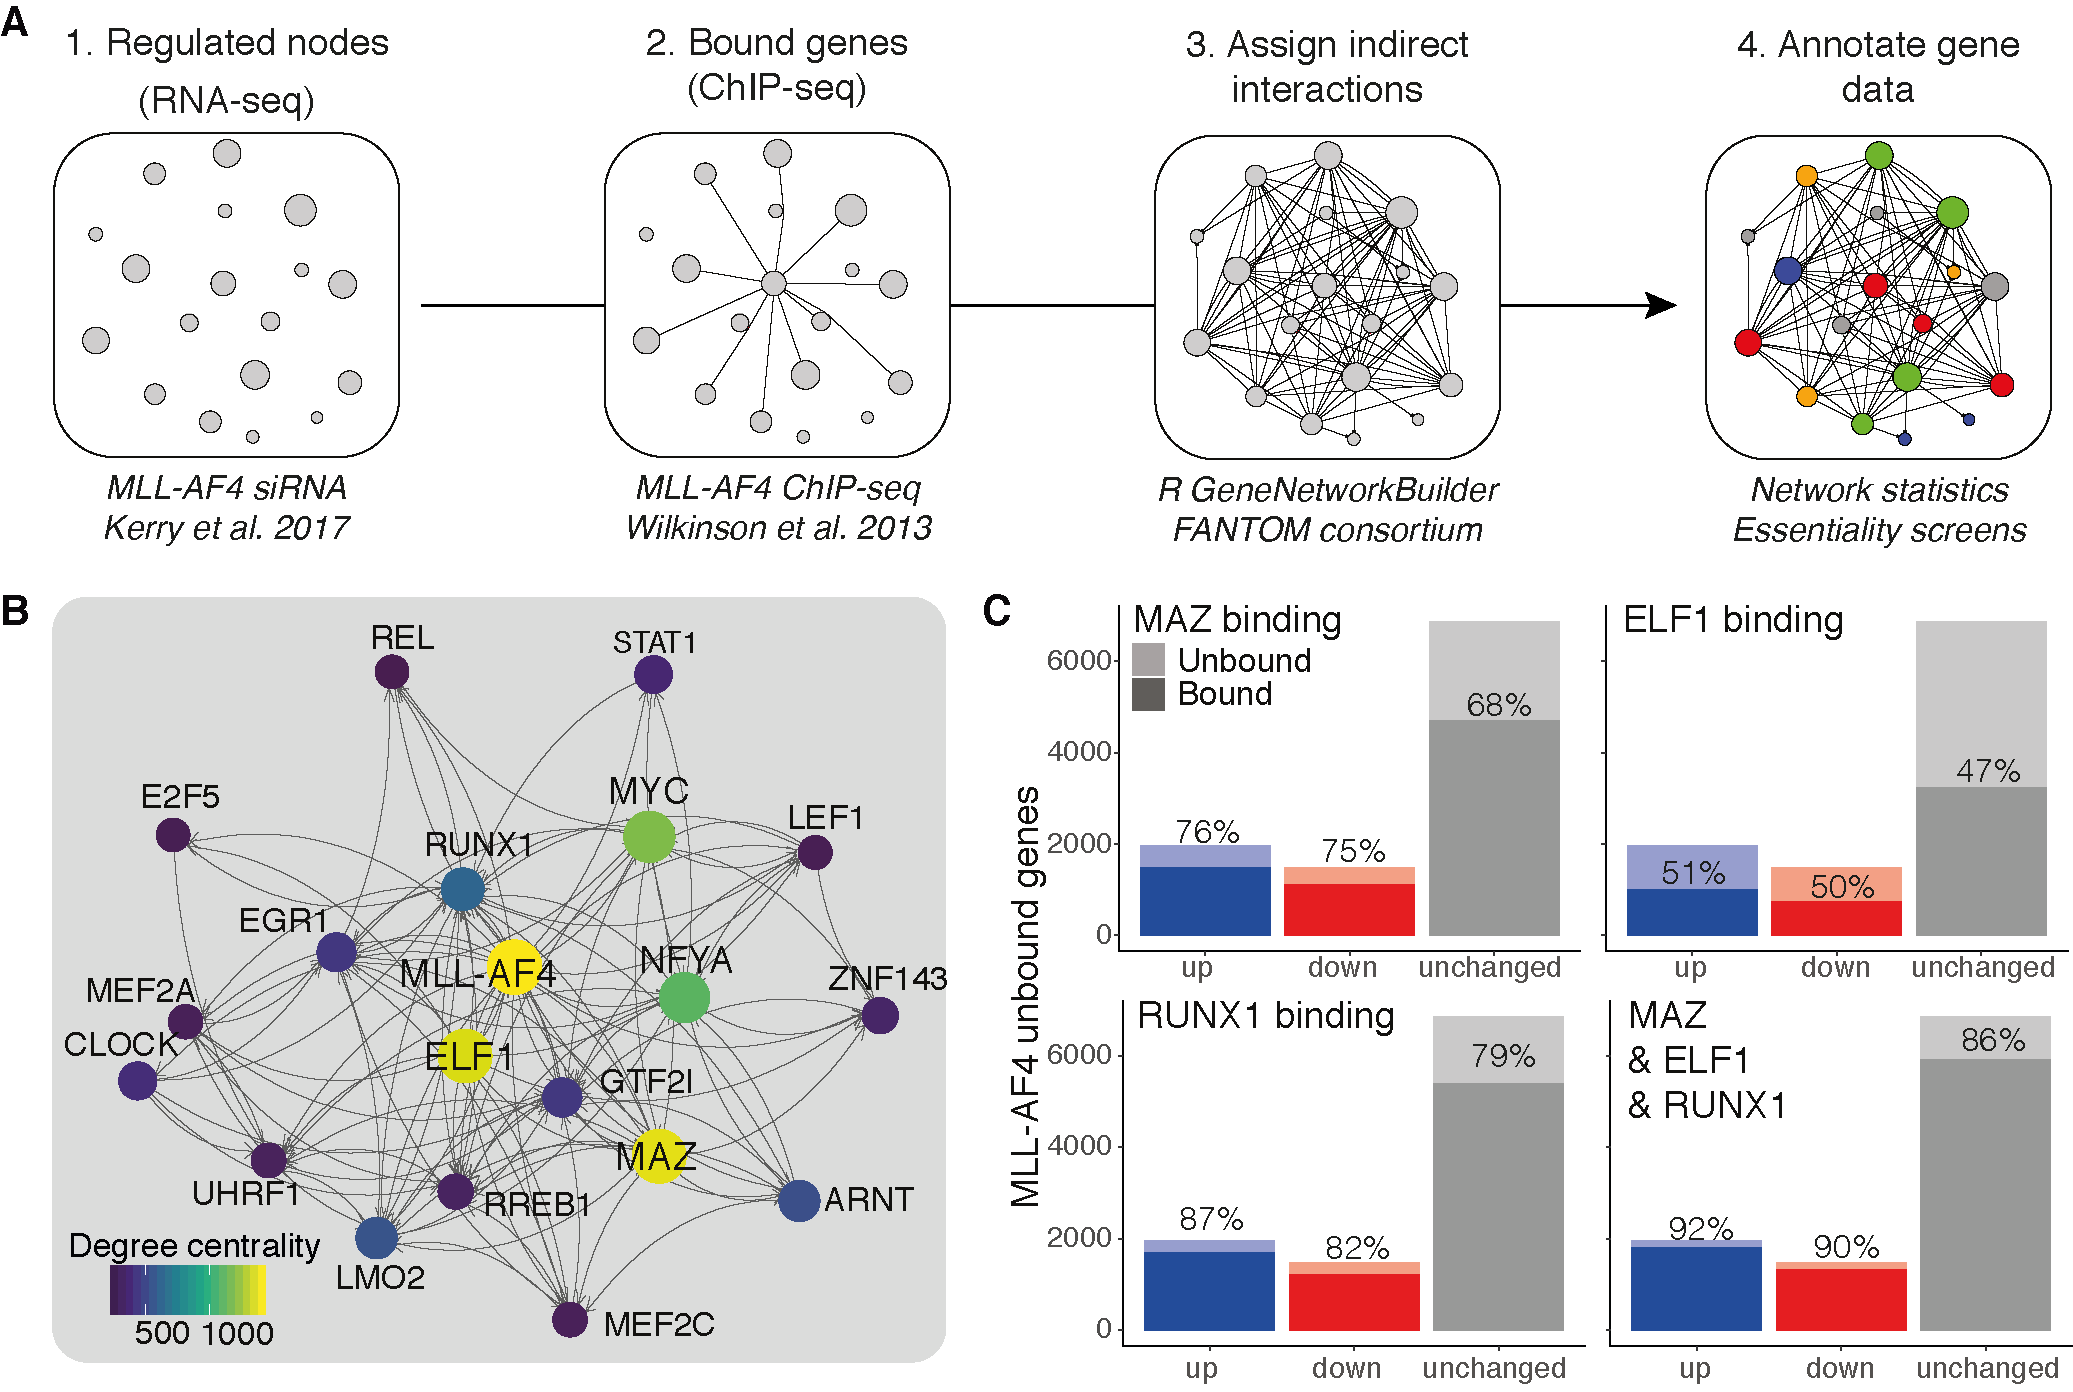
\includegraphics[width=\textwidth,height=\textheight,keepaspectratio]{figures/chapter4/ch4_ma4-grn.png}
    %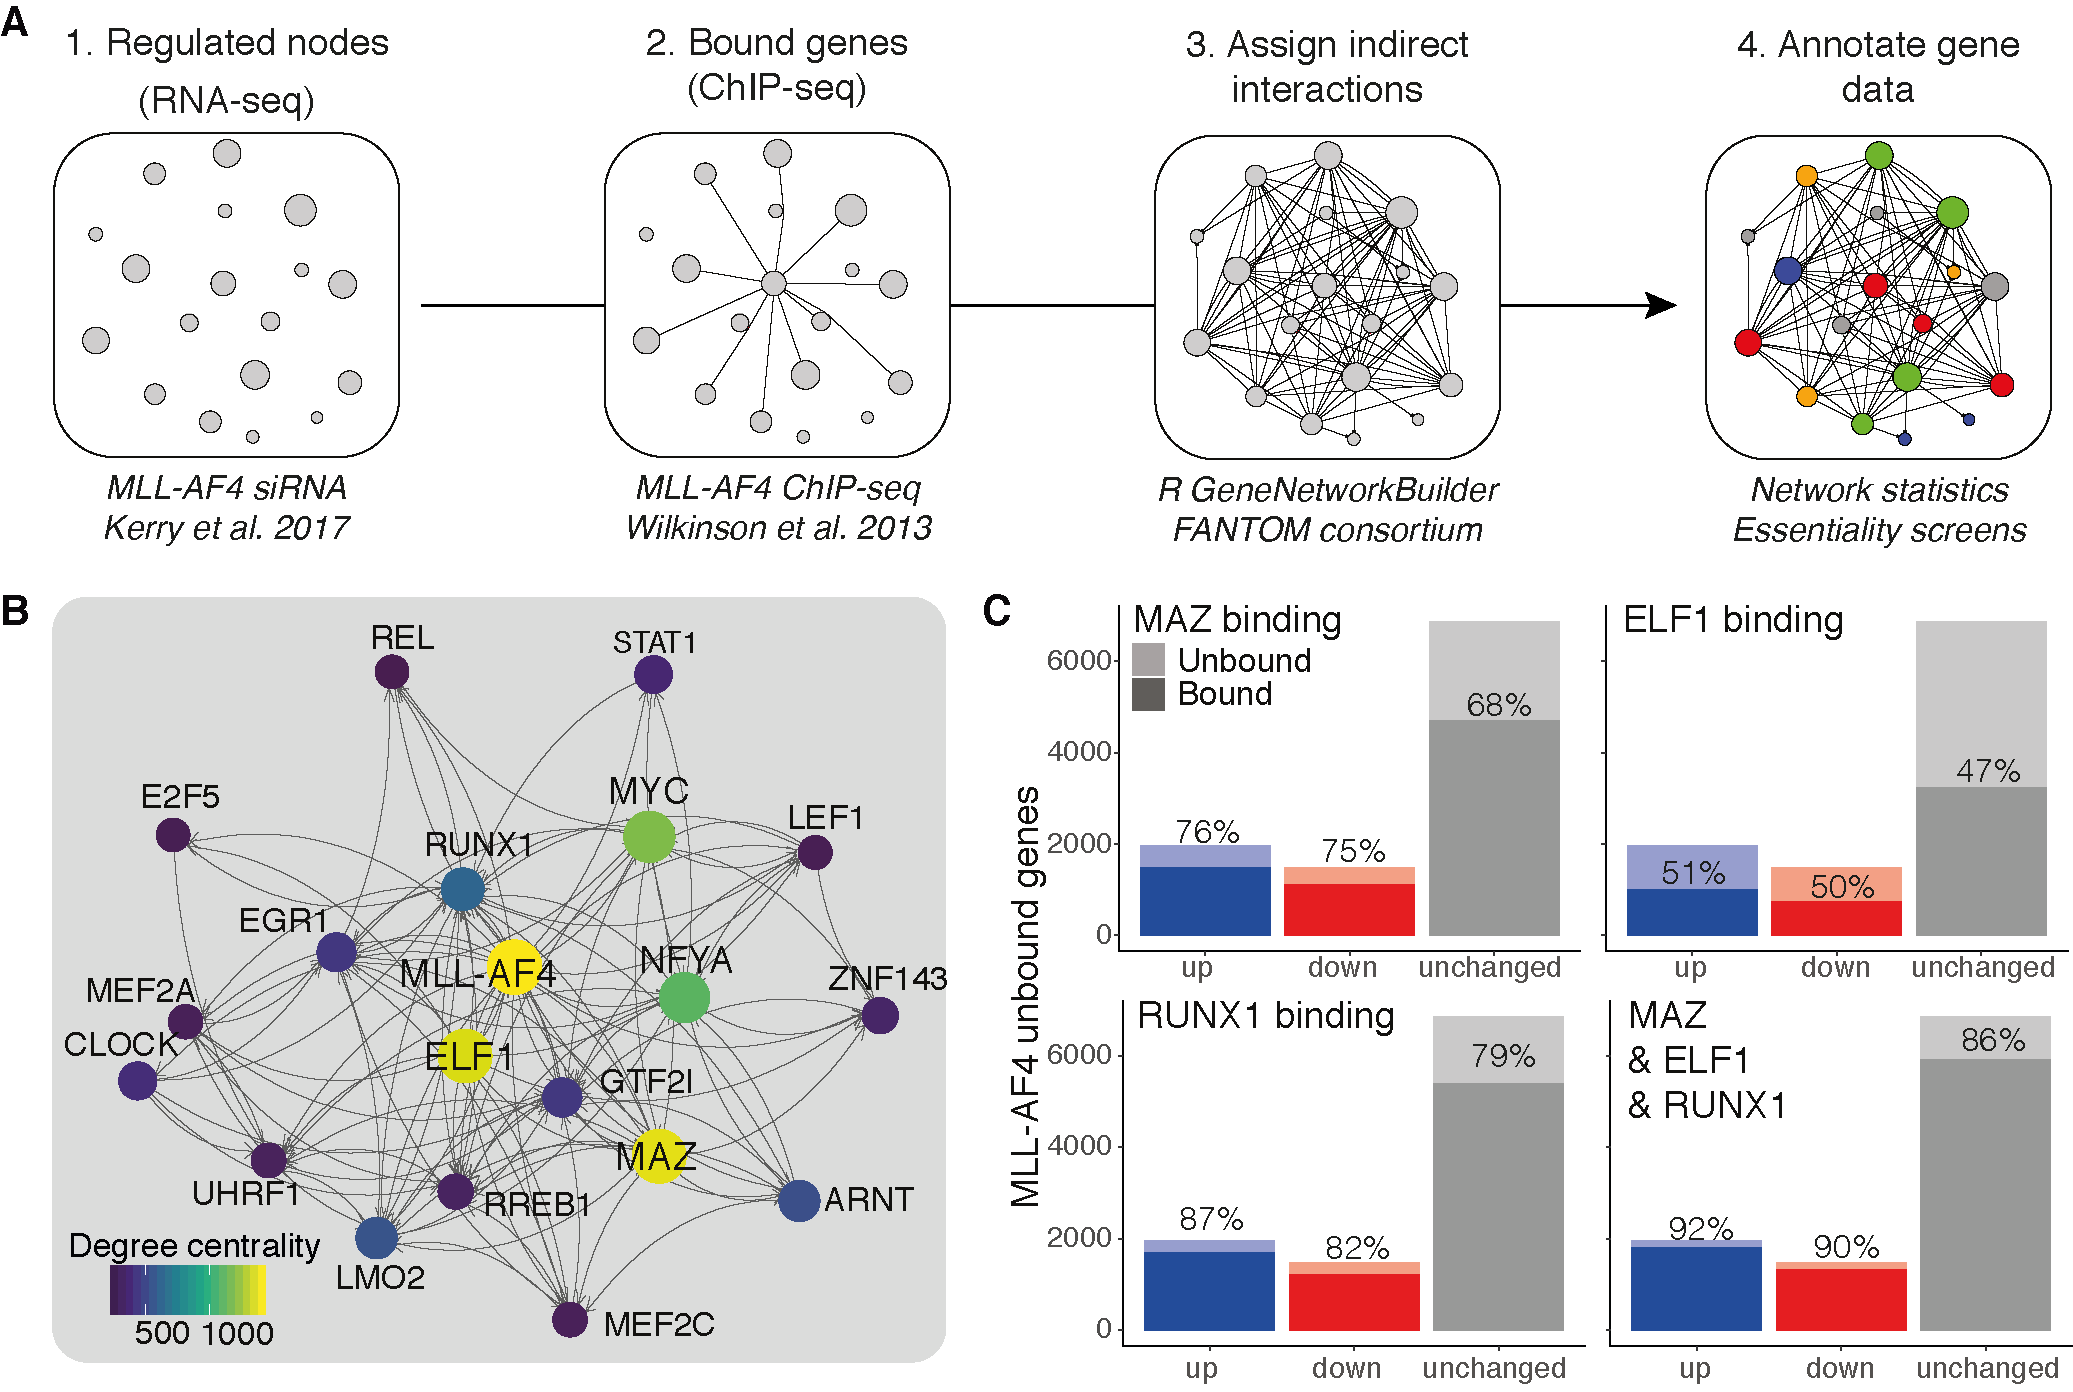
\includegraphics{figures/chapter4/ch4_ma4-grn.png}
    \caption[{Constructing an MLL-AF4 centred GRN model of MLL-AF4 leukaemia.}]
    {\textbf{Constructing an MLL-AF4 centred GRN model of MLL-AF4 leukaemia.} 
    \textbf{(A)} GRN creation workflow using siRNA KD with nascent RNA-seq, ChIP-seq, an underlying TF motif network \citep{the_fantom_consortium_and_the_riken_omics_science_center_transcriptional_2009}.
    \textbf{(B)} The top 20 genes of the MLL-AF4 GRN by degree centrality. Lines indicate predicted interaction from protein to gene locus, with arrowheads pointing downstream.
    \textbf{(C)} Number of \textit{MLL-AF4} KD DEGs that are not bound by MLL-AF4, as highlighted in Fig. \ref{fig:ch4_GRN_just}A. Shaded bars represent proportion of TF-bound DEGs. 
    \textit{Adapted from \cite{harman_kmt2a-aff1_2021}.}
    }
    \label{fig:ch4_ma4-grn}
\end{figure}

As the central hypothesis of this chapter suggests that indirectly regulated MLL-AF4 targets are affected through activated TFs, MLL-AF4 regulated TFs in the GRN must therefore bind to these indirect targets. Within the GRN a number of highly central TFs were found to be directly regulated by MLL-AF4, including ELF1, MAZ, MYC, NF-YA and RUNX1 (Fig. \ref{fig:ch4_ma4-grn}C). The Milne lab has previously shown \textit{ELF1} and \textit{RUNX1} to be MLL-AF4 targets, with a role in leukaemia \citep{godfrey_dot1l_2019, wilkinson_runx1_2013}. Interestingly, Elf1 was also identified as a central regulator for pre-HSCs in the EHT GRN (Fig. \ref{fig:ch3_centrality}, p.\pageref{fig:ch3_centrality}), suggesting that this role may be co-opted by MLL-AF4 in leukaemia. While MAZ has not previously been implicated in \textit{MLL}r leukaemias, it is known to bind and regulate \textit{MYC} \citep{komatsu_maz_1997}. MYC has a well-studied and critical role in many cancers \citep{dang_myc_2012}, supporting its place as a central TF here. NF-YA has been recently reported to have a role in \textit{MLL}r leukaemias, in that it may mediate binding of the MLL-FP complex component Menin, and subsequently the MLL-FP complex, to DNA. Inhibition of NF-YA may function synergistically with Menin-MLL1 inhibitors \citep{soto-feliciano_molecular_2022}. Taking ELF1, RUNX1 and MAZ as examples, the binding profiles of these central TFs can account for the majority of MLL-AF4 indirectly regulated targets, and their combined binding profile has the potential to regulate over 90\% of MLL-AF4 KD DEGs (Fig. \ref{fig:ch4_ma4-grn}D), highlighting the utility of this model for interrogating the wider regulatory scope of MLL-AF4.

\begin{figure}[!t]
    \centering
    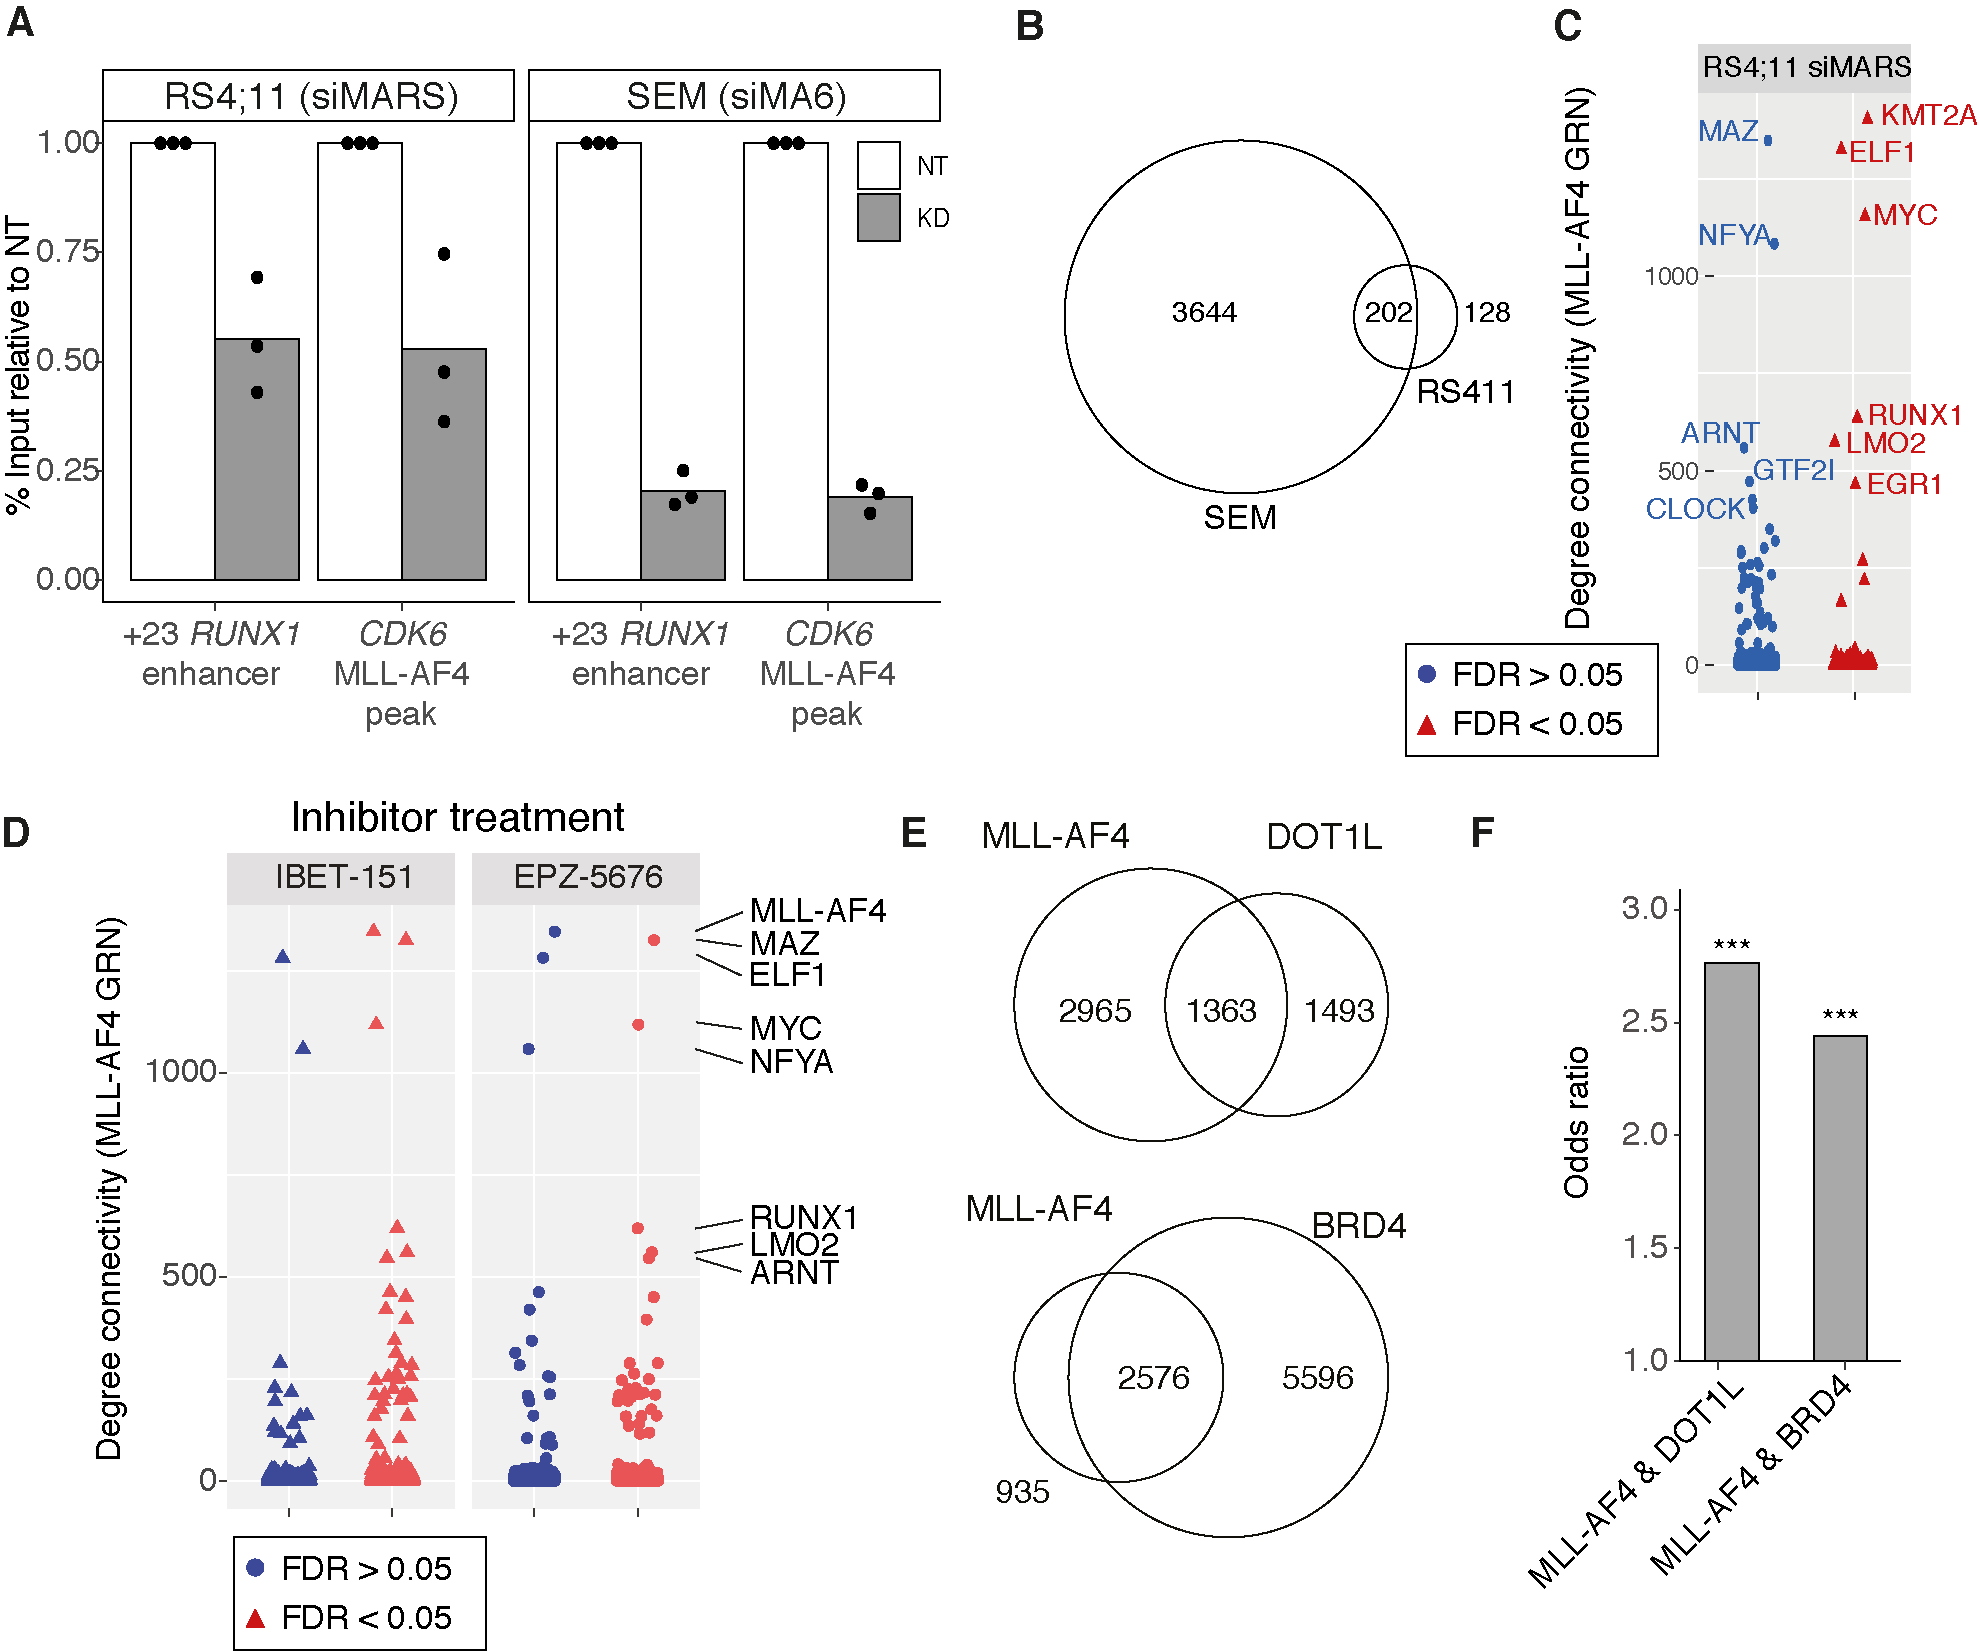
\includegraphics[width=\textwidth,height=\textheight,keepaspectratio]{figures/chapter4/ch4_grn-rs411.png}
    %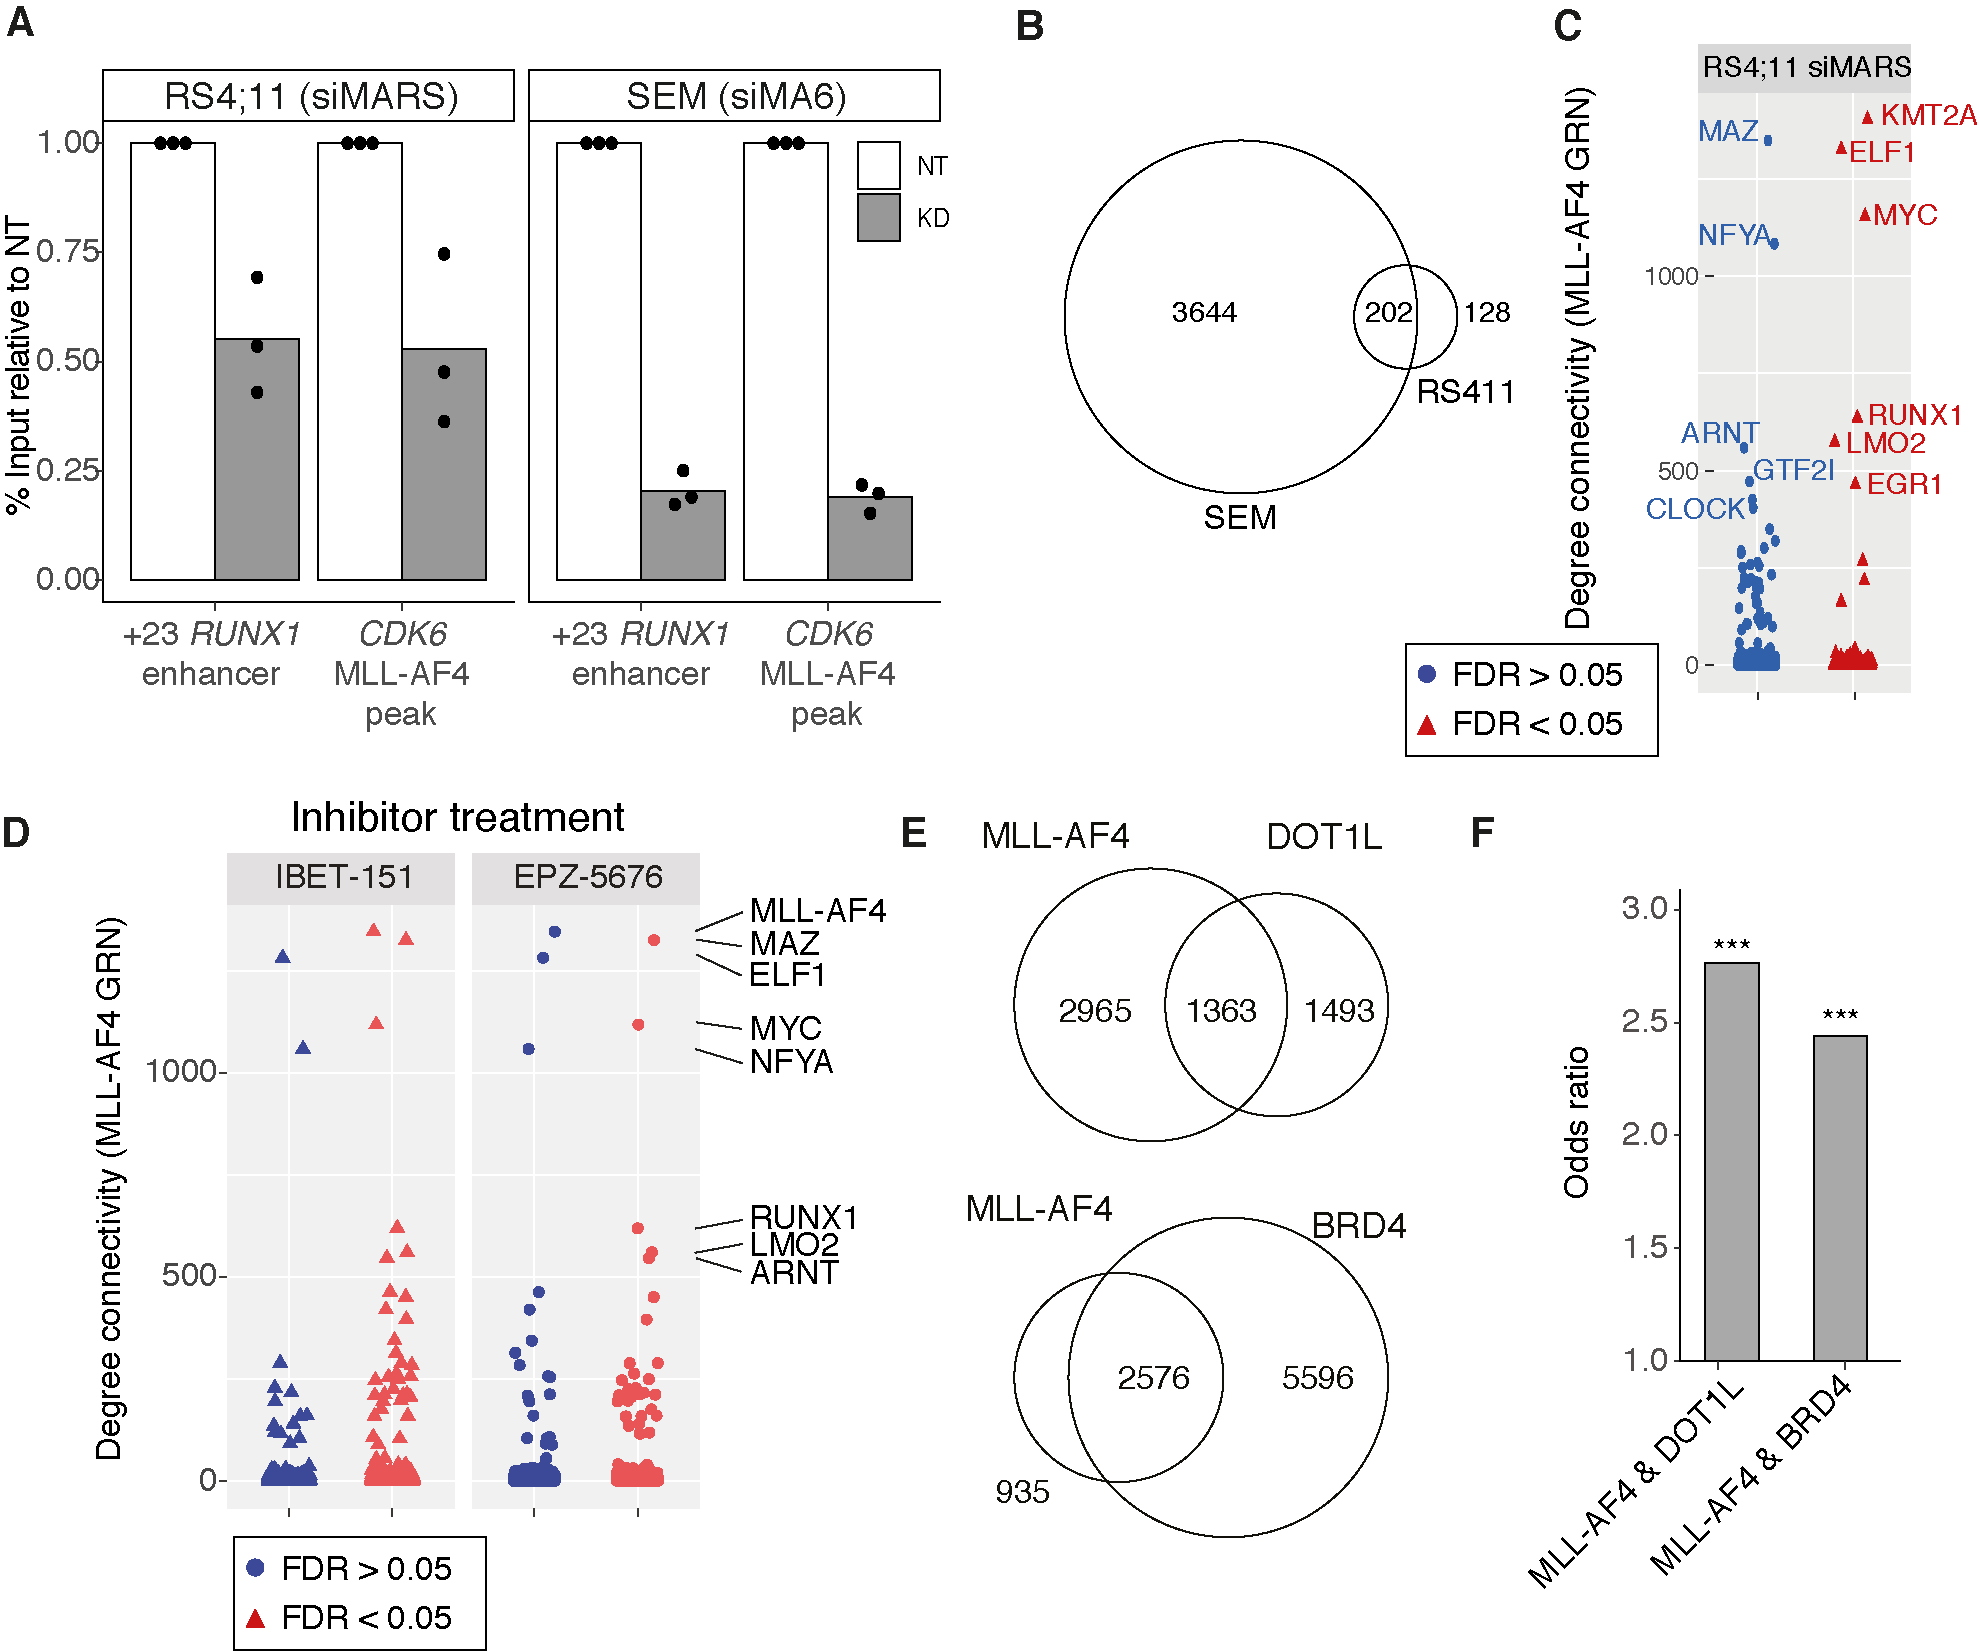
\includegraphics{figures/chapter4/ch4_grn-rs411.png}
    \caption[{Validation of the MLL-AF4 GRN.}]
    {\textbf{Validation of the MLL-AF4 GRN.} 
    \textbf{(A)} MLL-N ChIP-qPCR data in RS4;11 and SEM cells after \textit{MLL-AF4} KD, normalized to input chromatin and displayed relative to non-targeting (NT) control. siMA6 and siMARS refer to SEM and RS4;11 specific \textit{MLL-AF4} siRNA, respectively \citep{thomas_targeting_2005}. 
    \textbf{(B)} Overlap of nodes between SEM GRN and RS4;11 \textit{MLL-AF4} KD DEGs. 
    \textbf{(C-D)} Number of DEGs after \textit{MLL-AF4} KD in RS4;11 cells (\textit{n} = 3) (C), or  1.5 hours’ IBET and 7 days’ EPZ-5676 treatment (\textit{n} = 3) (D), plotted against degree centrality in the SEM MLL-AF4 GRN. Blue points: FDR > 0.05, red points: FDR < 0.05. 
    \textbf{(E)} Overlap of nodes between MLL-AF4 GRN, and IBET-151 and EPZ-5676 treatment DEGs. 
    \textbf{(F)} Fisher's exact test of overlaps shown in (E), showing odds ratios. (***) P < 0.001. 
    \textit{Raw data for D-F was generated previously in the Milne lab, and analysed by me. Adapted from \cite{harman_kmt2a-aff1_2021}.} 
    }
    \label{fig:ch4_grn-rs411}
\end{figure}

To validate this GRN model with an alternative MLL-AF4 ALL cell line, I determined how sensitive the GRN nodes are to \textit{MLL-AF4} perturbation in RS4;11 cells. I performed 96 hours' \textit{MLL-AF4} KD in both RS4;11 and SEM cells, and followed this with nascent RNA-seq. The siRNA designed for the MLL-AF4 breakpoint in RS4;11 was much less efficient than the siRNA for SEM cells, despite equivalent treatment conditions (Fig. \ref{fig:ch4_grn-rs411}A). This reduced efficacy has been observed in other studies \citep{thomas_targeting_2005, geng_integrative_2012}. Despite this reduced effectiveness of the siRNA, nascent RNA-seq analysis identified 330 DEGs, and 202 of these overlapped with the SEM MLL-AF4 GRN (Fig. \ref{fig:ch4_grn-rs411}B). Importantly, even in this reduced network many of the most central GRN nodes were still affected upon RS4;11 \textit{MLL-AF4} KD, including \textit{RUNX1}, suggesting that these central factors are highly sensitive and consistent across MLL-AF4 ALL cell lines (Fig. \ref{fig:ch4_grn-rs411}C). 

To further validate the GRN, I tested whether the GRN nodes reflect activity of MLL-AF4 complex components. DOT1L is a core complex factor \citep{bernt_mll-rearranged_2011, biswas_function_2011, lacoste_disruptor_2002, milne_leukemogenic_2005, okada_hdot1l_2005, mueller_role_2007, slany_mll_2020, lin_instructive_2016, krivtsov_h3k79_2008} that should strongly overlap with the GRN, and BRD4 is an associated cofactor with a general role in gene activation \citep{dawson_inhibition_2011, zuber_rnai_2011} that is not specific to the MLL-AF4 complex. Comparing the MLL-AF4 GRN with DEGs following 7 days’ EPZ-5676 (DOT1L inhibitor) treatment and 1.5 hours’ IBET-151 (BRD4 inhibitor) treatment (Published data from \cite{godfrey_dot1l_2019} and \cite{crump_bet_2021}), both inhibitors overlapped with the GRN and impacted central TFs (Fig. \ref{fig:ch4_grn-rs411}D-E). DOT1L inhibition impacted less of the MLL-AF4 GRN than BRD4, but with greater specificity (Fig. \ref{fig:ch4_grn-rs411}F). This analysis serves to validate that the MLL-AF4 GRN represents aspects of BRD4 and DOT1L activity and is therefore a reliable representation of MLL-AF4 complex behaviour.

\section[Integrating patient expression data highlights regulatory modules, and a set of “core” MLL-FP TFs]{\label{ch4:patient}Integrating patient expression data highlights regulatory modules, and a set of “core”\\MLL-FP TFs}

\begin{figure}[!t]
    \centering
    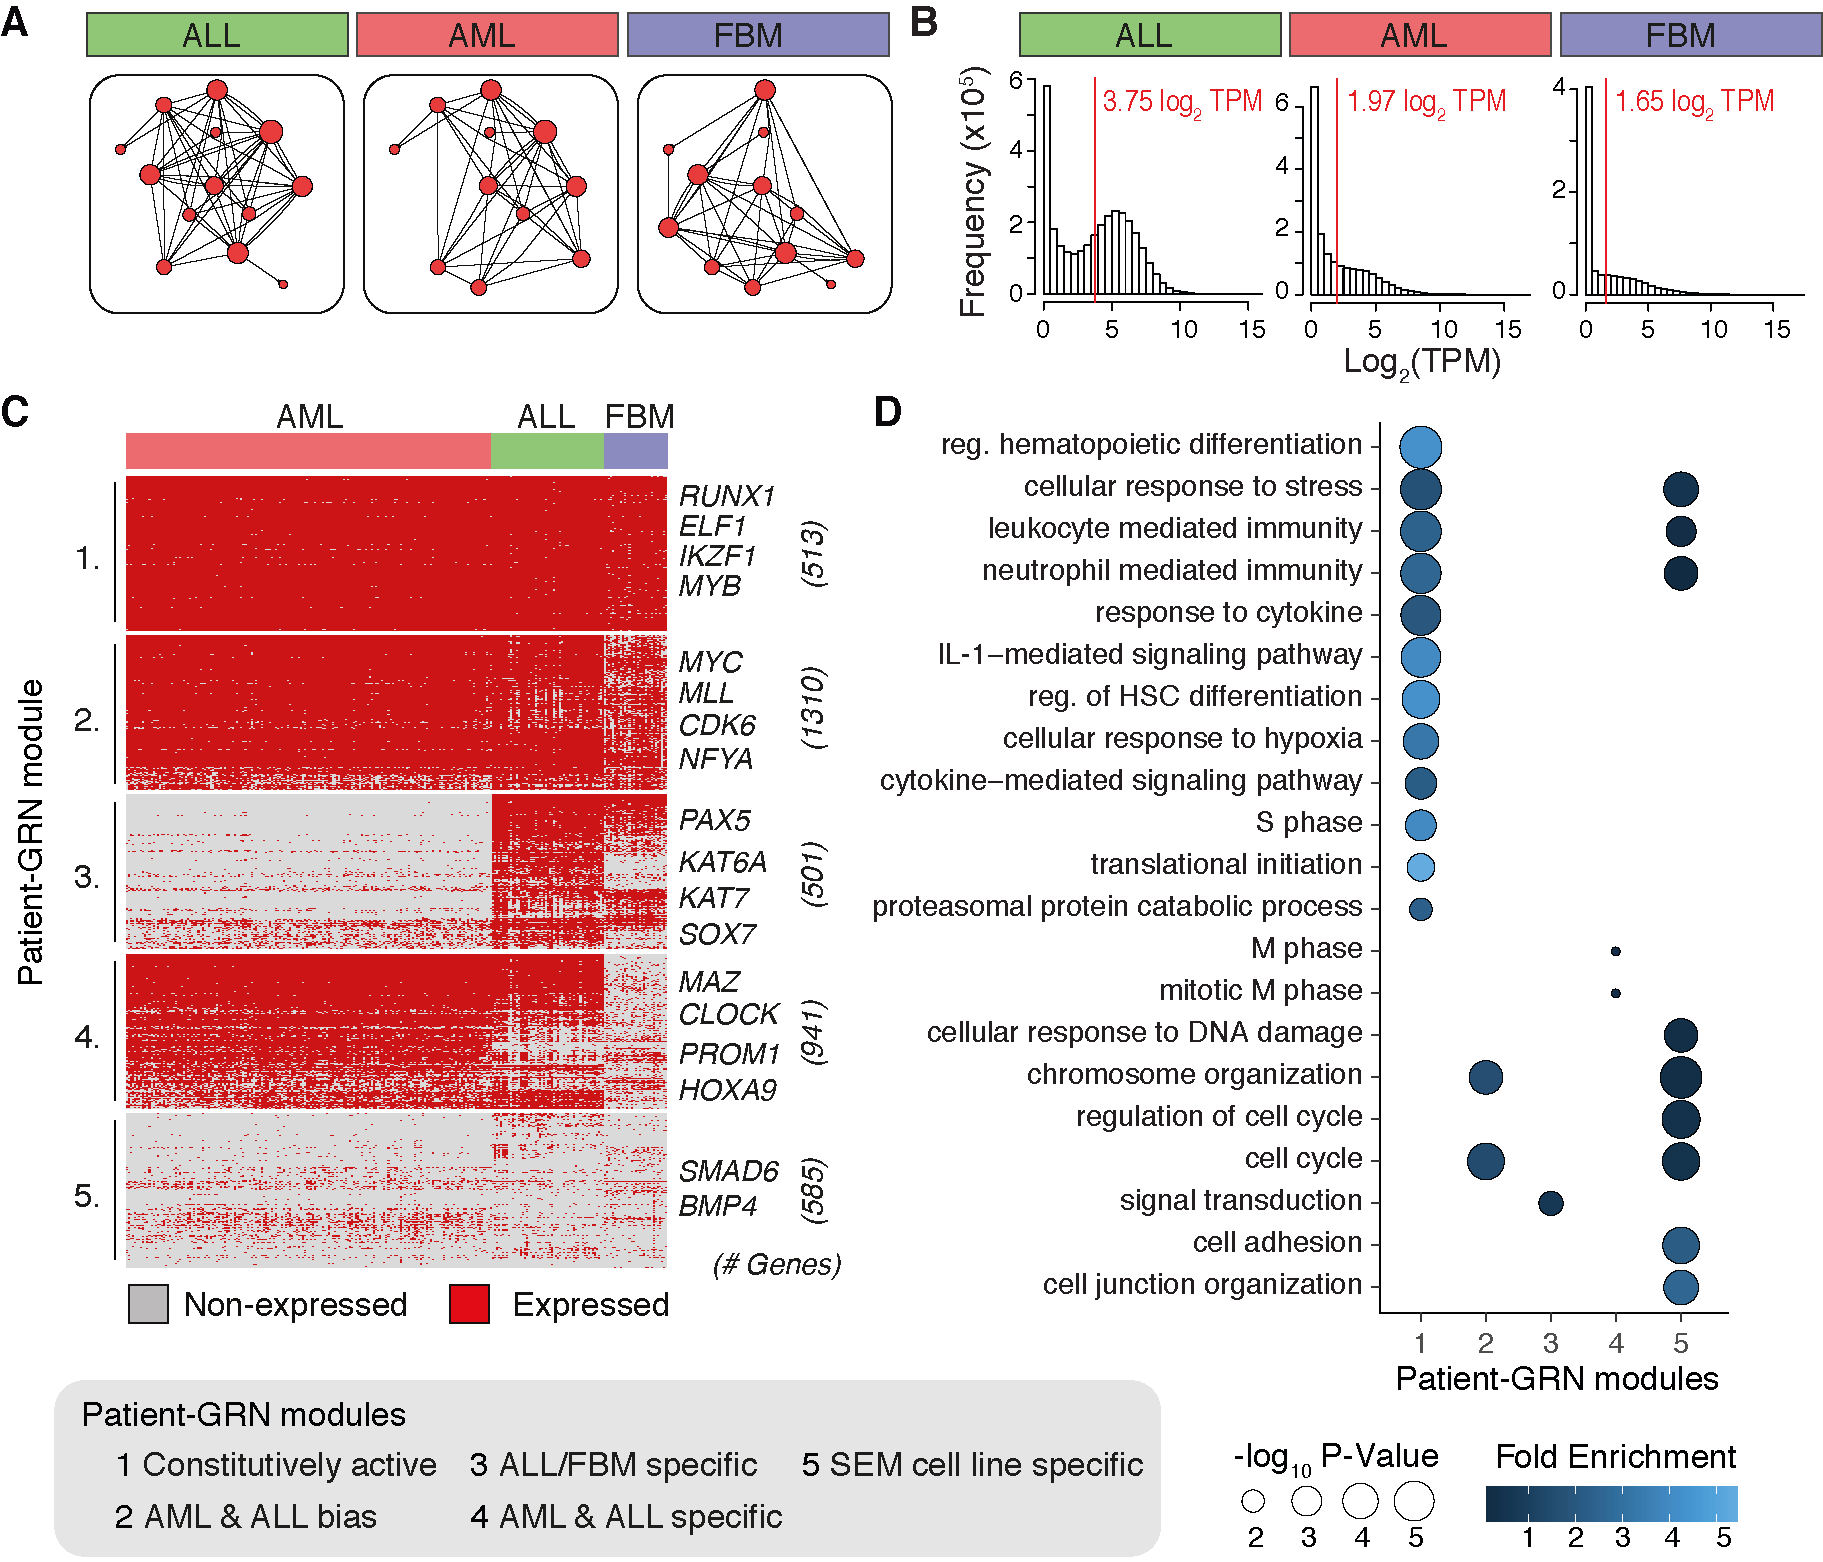
\includegraphics[width=\textwidth,height=\textheight,keepaspectratio]{figures/chapter4/ch4_patient.png}
    %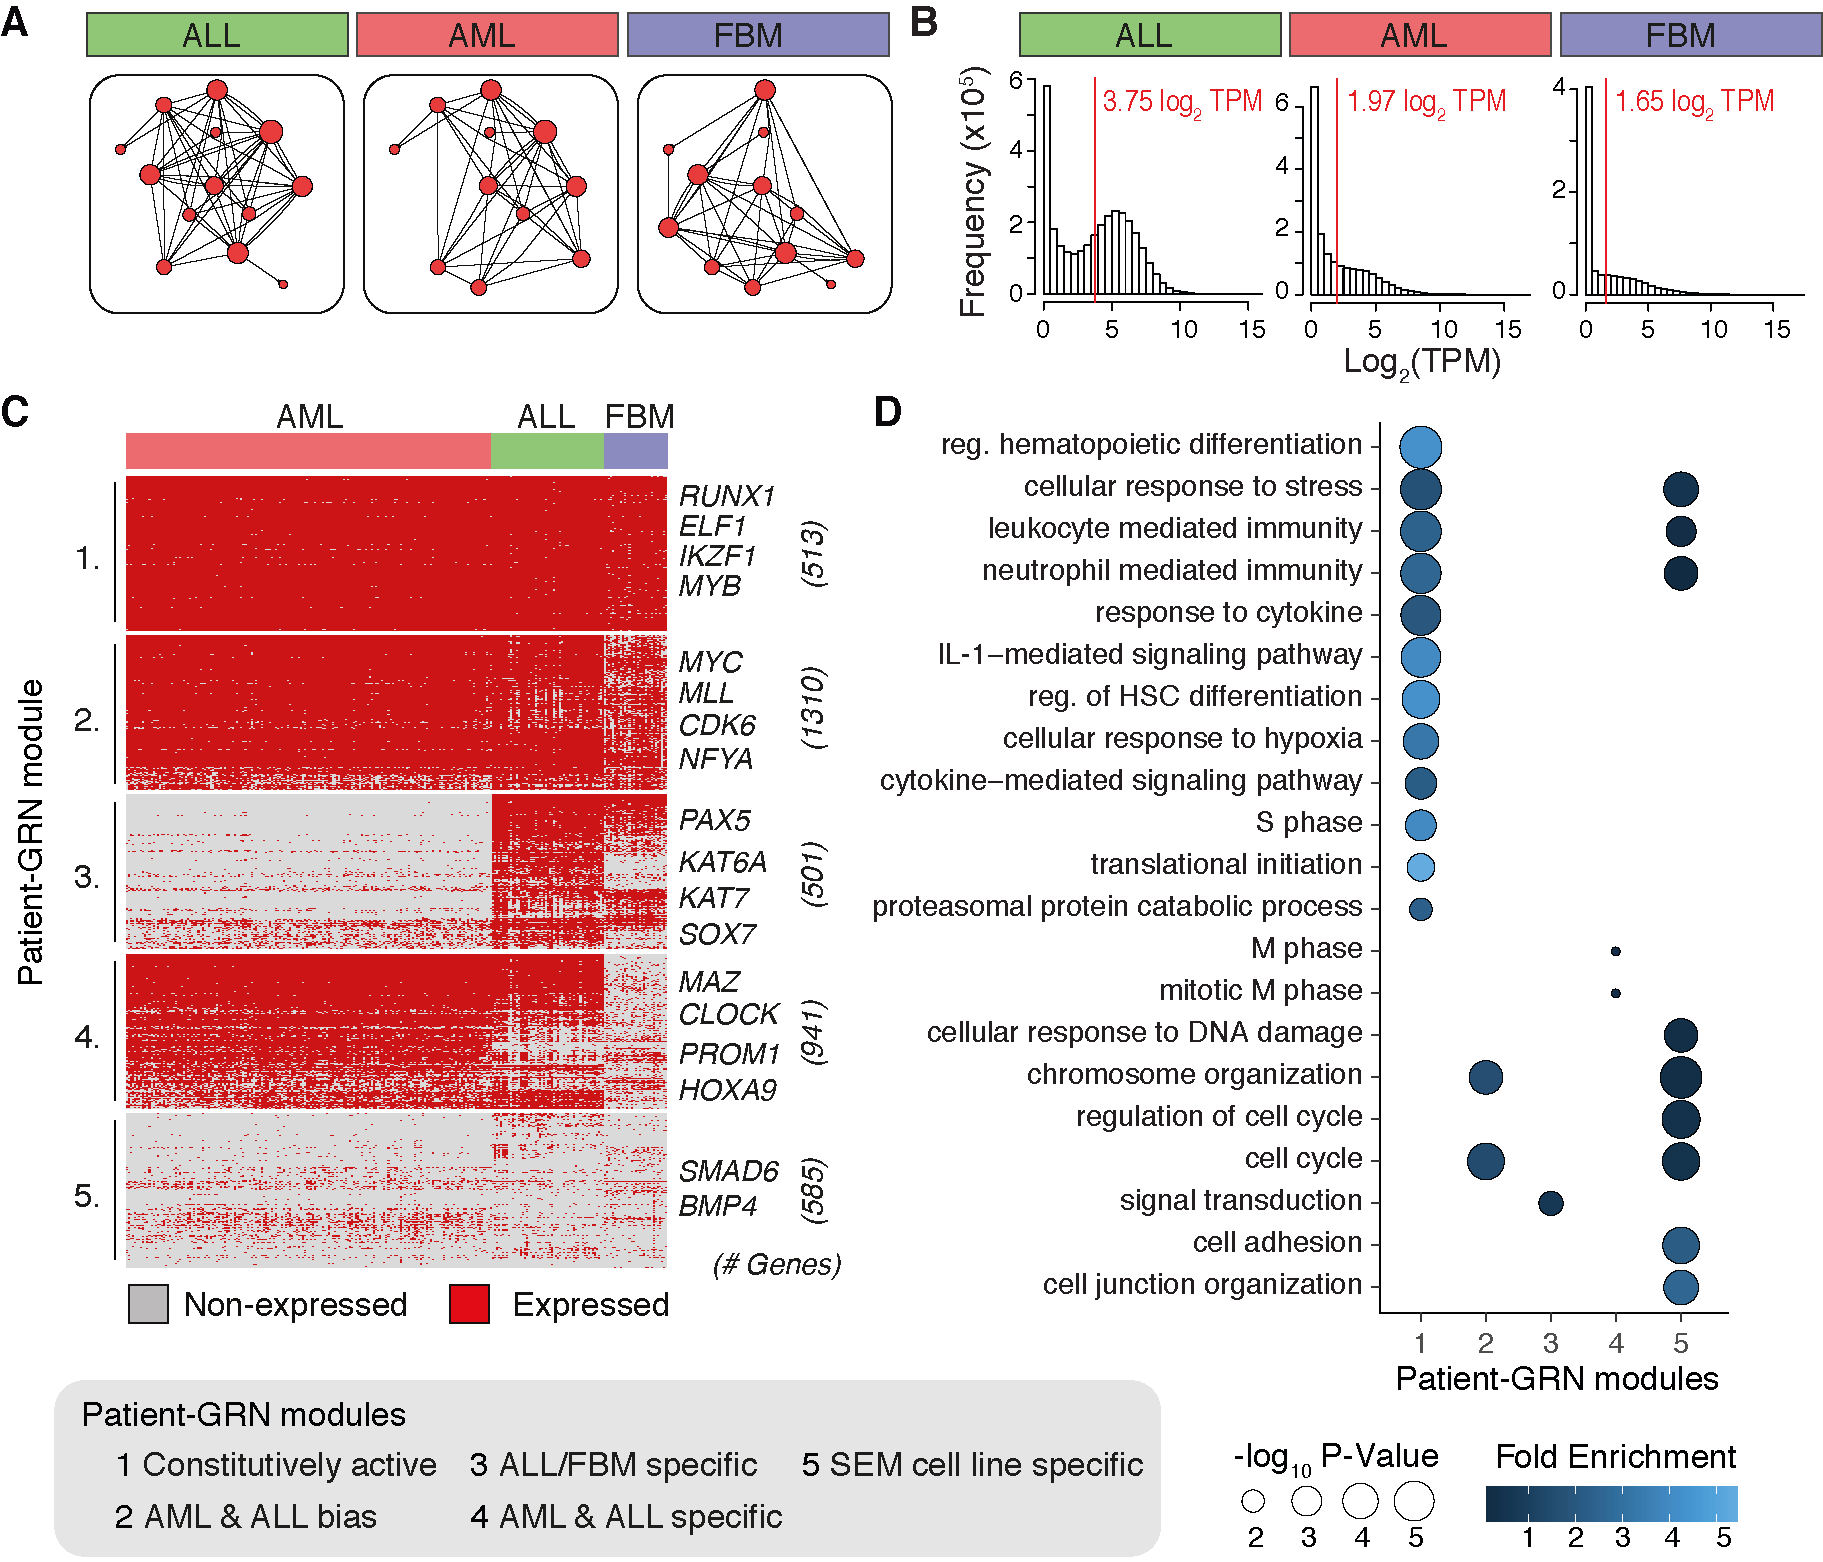
\includegraphics{figures/chapter4/ch4_patient.png}
    \caption[{The MLL-AF4 GRN can be split into regulatory modules based on patient gene expression.}]
    {\textbf{The MLL-AF4 GRN can be split into regulatory modules based on patient gene expression.} 
    \textbf{(A)} Schematic illustration of sub-networks reflecting expressed genes in patient samples. 
    \textbf{(B)} Histograms of log\textsubscript{2} TPM expression in AML, ALL and FBM datasets. Red line indicates threshold for defining active gene expression (mean log\textsubscript{2} TPM). 
    \textbf{(C)} GRN node activity across sub-networks as defined in B. Genes were grouped into patient-GRN modules using \textit{k}-means. Rows represent genes; columns represent samples. 
    \textbf{(D)} GO biological process enrichment for patient-GRN modules. 
    \textit{Normalised expression data for this analysis was sourced from published data, with GRN analyses performed by me. Adapted from \cite{harman_kmt2a-aff1_2021}.}
    }
    \label{fig:ch4_patient}
\end{figure}

\textit{MLL} translocations can involve many different fusion partners, and can result in either ALL or AML. There are also cases where lineage switching occurs after relapse \citep{dorantes-acosta_lineage_2012, gardner_acquisition_2016}. This suggests similarity in the behaviour across different MLL-FP complexes, in both ALL and AML lineages, and suggests there may be a core set of targets driven by MLL-FPs more generally. Further, the translocation events often occur in utero resulting in infant and childhood leukaemias \citep{greaves_causal_2018, greaves_utero_2005, ford_utero_1993, jackson_origin_2021}, and fetal programs can be overexpressed in \textit{MLL}r leukaemia \citep{rice_human_2021}, indicating that the MLL-AF4 GRN originates in a fetal regulatory landscape. To assess whether the GRN model represents common ALL and AML biology, or shares characteristics with fetal B-cell development, I overlapped the GRN with patient and fetal bone marrow (FBM) expression data to create sub-networks (Fig. \ref{fig:ch4_patient}A). Expression data was taken from \textit{MLL}r ALL patients \citep{agraz-doblas_unraveling_2019}, AML patients with various chromosomal abnormalities \citep{the_cancer_genome_atlas_research_network_genomic_2013}, and HSPCs and B cells from normal FBM \citep{obyrne_discovery_2019}. These FBM populations included HSCs, multipotent progenitors (MPP), lympho-myelo primed progenitors (LMPP), pre-pro-B and pro-B cells. A threshold was used to define active genes, based on the mean gene expression within each dataset. Active genes were used to filter the MLL-AF4 GRN into patient specific sub-networks (Fig. \ref{fig:ch4_patient}B, methods section \ref{ch2:ma4-grn}, p.\pageref{ch2:ma4-grn}). Median expression was unusable due to low sequencing depth in the FBM data.

\subsection{\label{ch4:patient-modules}Regulatory modules of the GRN}

A binary matrix of gene activity across sub-networks was generated, then clustered into five patient-GRN modules (Fig. \ref{fig:ch4_patient}C). Note that \textit{MLL} expression in the case of \textit{MLL}r leukaemias also includes MLL-FP activity. A caveat of this analysis is that levels of expression are not addressed, which may have more subtle but important consequences. For example, \textit{RUNX1} is present in module 1 and active across all samples, however \textit{RUNX1} has been shown to be overexpressed in MLL-AF4 ALLs compared to MLL-AF9 AML and is important for leukaemic growth \citep{wilkinson_runx1_2013}. Thus, expression level rather than simply just presence of gene expression is likely an important indicator of functional importance. Nevertheless, this analysis serves to highlight modules that are potentially important across multiple leukaemias. 

Nodes in modules 1 and 2 are active across all leukaemias and FBM populations and are associated with haematopoietic differentiation as a key process, emphasising a maintained fetal haematopoietic program (Fig. \ref{fig:ch4_patient}D). Module 3 is active in ALL and a subset of FBM samples, and identifies \textit{SOX7} and \textit{KAT6A} as ALL-specific, and \textit{PAX5} and \textit{KAT7} in both ALL and FBM (Fig. \ref{fig:ch4_patient}C). The lack of AML activity implies this module differentiates ALL and AML, reinforced by the presence of \textit{PAX5}, a critical regulator of B lymphopoiesis \citep{medvedovic_pax5_2011}, and \textit{SOX7}, which is highly expressed in ALL over AML and drives proliferation \citep{cuvertino_sox7_2016}. Module 4 is instead active in both AML and ALL datasets, with low activity in FBM samples (Fig. \ref{fig:ch4_patient}C), indicating nodes distinct from the normal B progenitor program. Interestingly, this includes the central GRN node \textit{MAZ}, indicating it is a leukaemia specific target. \textit{PROM1} (CD133) is also in this cluster, which is normally expressed in more stem and progenitor cells but can be dramatically upregulated by MLL-FPs and is essential for many ALL leukaemias \citep{godfrey_h3k79me23_2021, mak_mixed_2012, obyrne_discovery_2019}. Module 5 is inactive across all datasets (Fig. \ref{fig:ch4_patient}C), and pathway enrichment shows terms related to cell junction organisation and adhesion, response to stress, and DNA damage response (Fig. \ref{fig:ch4_patient}D), which likely represents an immortalised cell program. Together, this analysis breaks down the MLL-AF4 GRN into different modules representing ALL specific, core AML and ALL, and B-lymphopoiesis co-opted circuits. ALL specific nodes are expected as an ALL based GRN, while nodes active in both ALL and FBM populations are suggestive of a B progenitor program maintained in ALL, which may be overactivated by MLL-AF4. A particularly interesting subset are nodes active in both ALL and AML. This is indicative of a program active in both lineages, and as \textit{MLL}r may undergo lineage switching, this may represent a consistent program that enables this switch to occur.

\subsection{\label{ch4:patient-core}High centrality nodes represent a core MLL-FP program}

As MLL-AF4 may regulate a core set of nodes across lineages (Fig. \ref{fig:ch4_patient}C), it is important to establish which TFs drive this core program. The most central nodes of the SEM MLL-AF4 GRN (degree centrality > 500) are active across all ALL and AML patient sub-networks (Fig. \ref{fig:ch4_core}A), suggesting these TFs play a common role across lineages. Central GRN nodes are considerably less conserved in the fetal B progenitor program (Fig. \ref{fig:ch4_core}A), suggesting that this is regulated by distinct TFs, although this could be a consequence of the low sequencing depth or diversity of fetal populations. Patient-GRN modules 1, 2 and 4 represent the core regulatory logic between acute leukaemias (Fig. \ref{fig:ch4_patient}C), and show strikingly higher centrality compared to modules 3 and 5 (Fig. \ref{fig:ch4_core}B). Therefore, the central factors of these clusters can be taken as a panel of core TFs applicable to both AML and ALL (Fig. \ref{fig:ch4_core}C).

\begin{figure}[!t]
    \centering
    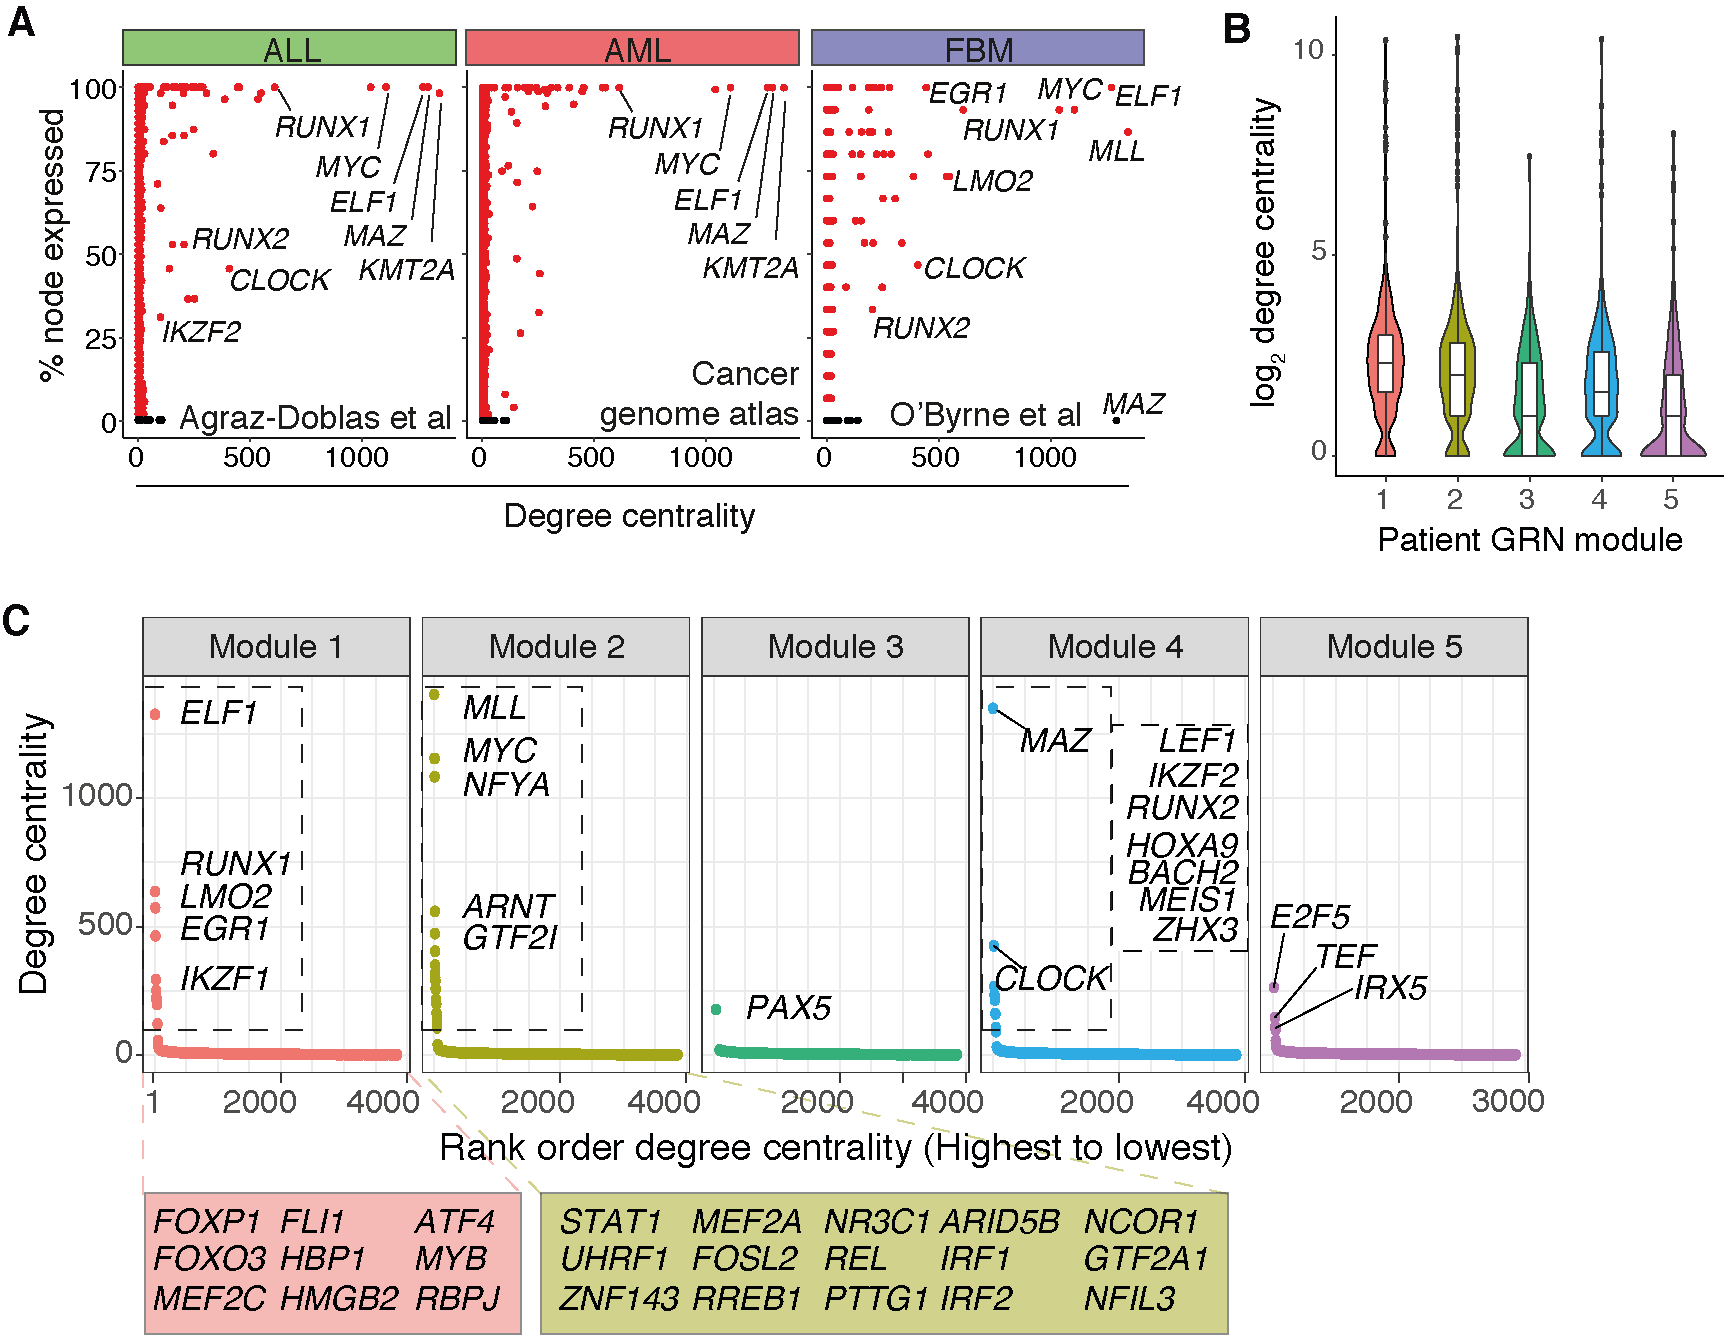
\includegraphics[width=\textwidth,height=\textheight,keepaspectratio]{figures/chapter4/ch4_core-nodes.png}
    %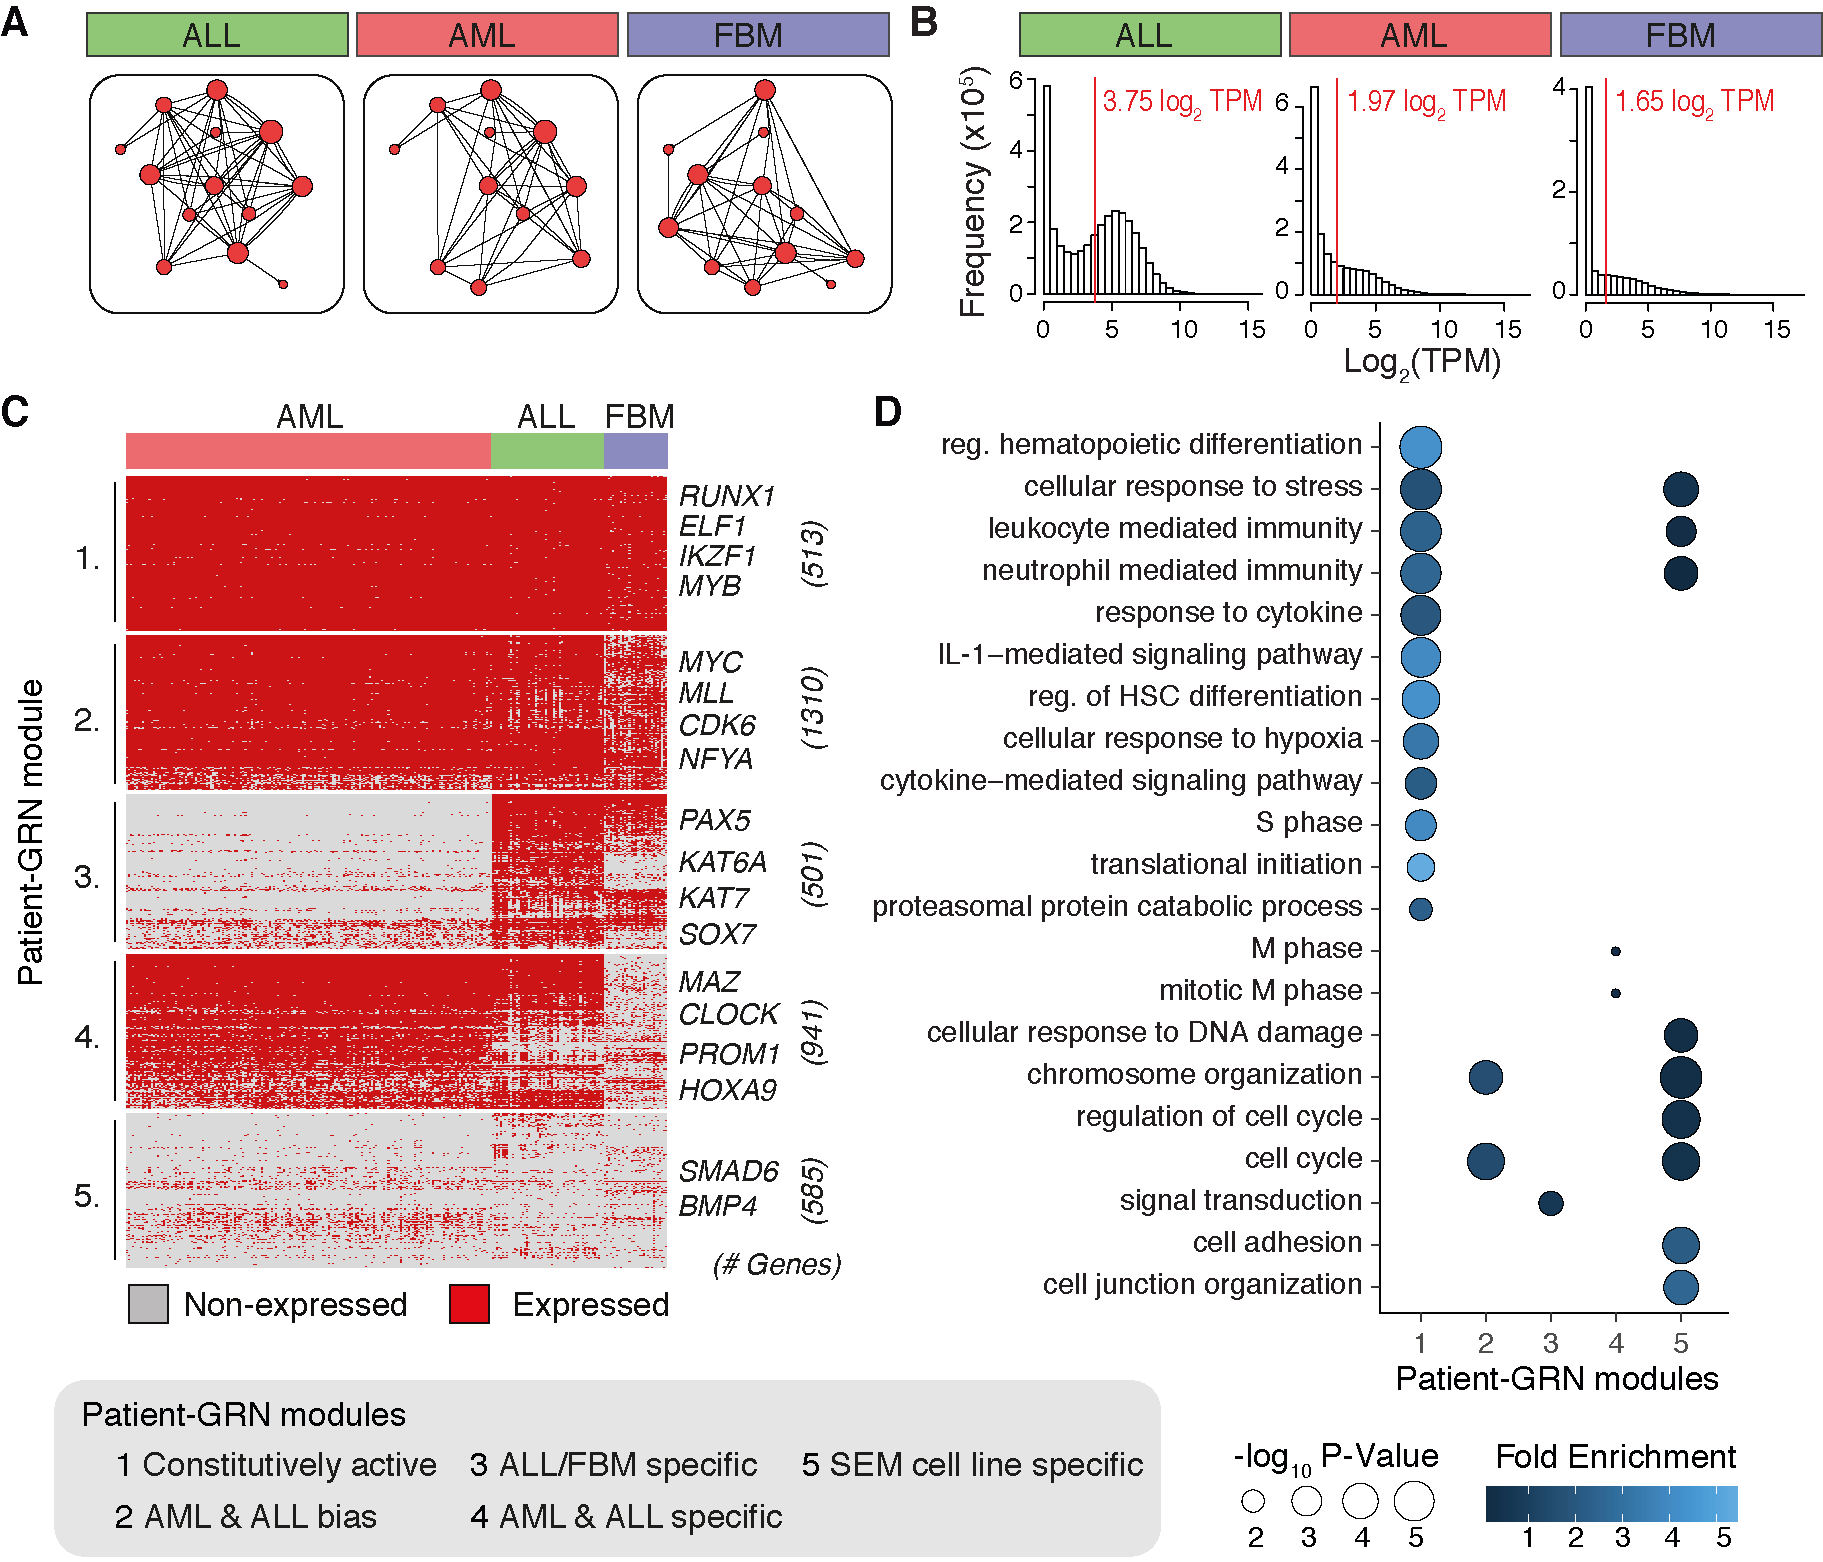
\includegraphics{figures/chapter4/ch4_patient.png}
    \caption[{Patient expression modules reveal a set of core, central nodes.}]
    {\textbf{Patient expression modules reveal a set of core, central nodes.} 
    \textbf{(A)} Relationship between percentage of patient samples expressing each gene and MLL-AF4 GRN centrality. 
    \textbf{(B)} Distribution of log\textsubscript{2} degree centrality of GRN nodes, stratified by patient-GRN module.  
    \textbf{(C)} Top-most GRN nodes by degree centrality, stratified by patient-GRN modules. Annotated nodes in Clusters 1, 2, and 4 represent the core TFs of the GRN model. 
    \textit{Adapted from \cite{harman_kmt2a-aff1_2021}.}
    }
    \label{fig:ch4_core}
\end{figure}

The analysis so far has identified highly connected TFs present across AML and ALL lineages. This has focused on the MLL-AF4 centred GRN, but our analysis could be extended to other MLL-FPs, such as MLL-AF9, to determine if there is a general MLL-FP core network. To test this, I compared MLL-N ChIP-seq profiles between SEM and THP-1 cells (MLL-AF9 AML). Of SEM MLL-AF4 bound genes in the MLL-AF4 GRN, 66\% are bound by MLL-AF9 in THP-1 cells (Fig. \ref{fig:ch4_sem-thp1}A). To determine whether this commonality extends to central targets of MLL-AF4, I performed the same comparison with RUNX1 ChIP-seq. Interestingly, only 35\% of SEM RUNX1 bound genes are in common with THP-1, suggesting that while there is common MLL-FP behaviour the central TFs are lineage specific (Fig. \ref{fig:ch4_sem-thp1}A). MLL-AF4 and MLL-AF9 binding profiles are broadly similar at common gene targets (Fig. \ref{fig:ch4_sem-thp1}B), with similar enhancer occupancy and MLL-FP spreading \citep{kerry_mll-af4_2017}. The core TF program is largely bound by MLL-FP in both SEM and THP-1 cells, with some exceptions including \textit{MAZ}, \textit{NFYA} and \textit{EGR1} (Fig. \ref{fig:ch4_sem-thp1}D). In contrast, RUNX1 binding profiles at enhancers differ, such as at the \textit{GFI1} locus (Fig. \ref{fig:ch4_sem-thp1}C). Despite these differences, many of the central GRN factors are bound by RUNX1 in both cell types (Fig. \ref{fig:ch4_sem-thp1}E). These analyses validate the capacity of the core MLL-FP TFs to regulate both ALL and AML leukaemias, using different MLL fusion partners, and highlight differences in RUNX1 binding between lineages. The core program of these leukaemias are similar, but the wider regulatory network may be context dependent.

\begin{figure}[htbp]
    \centering
    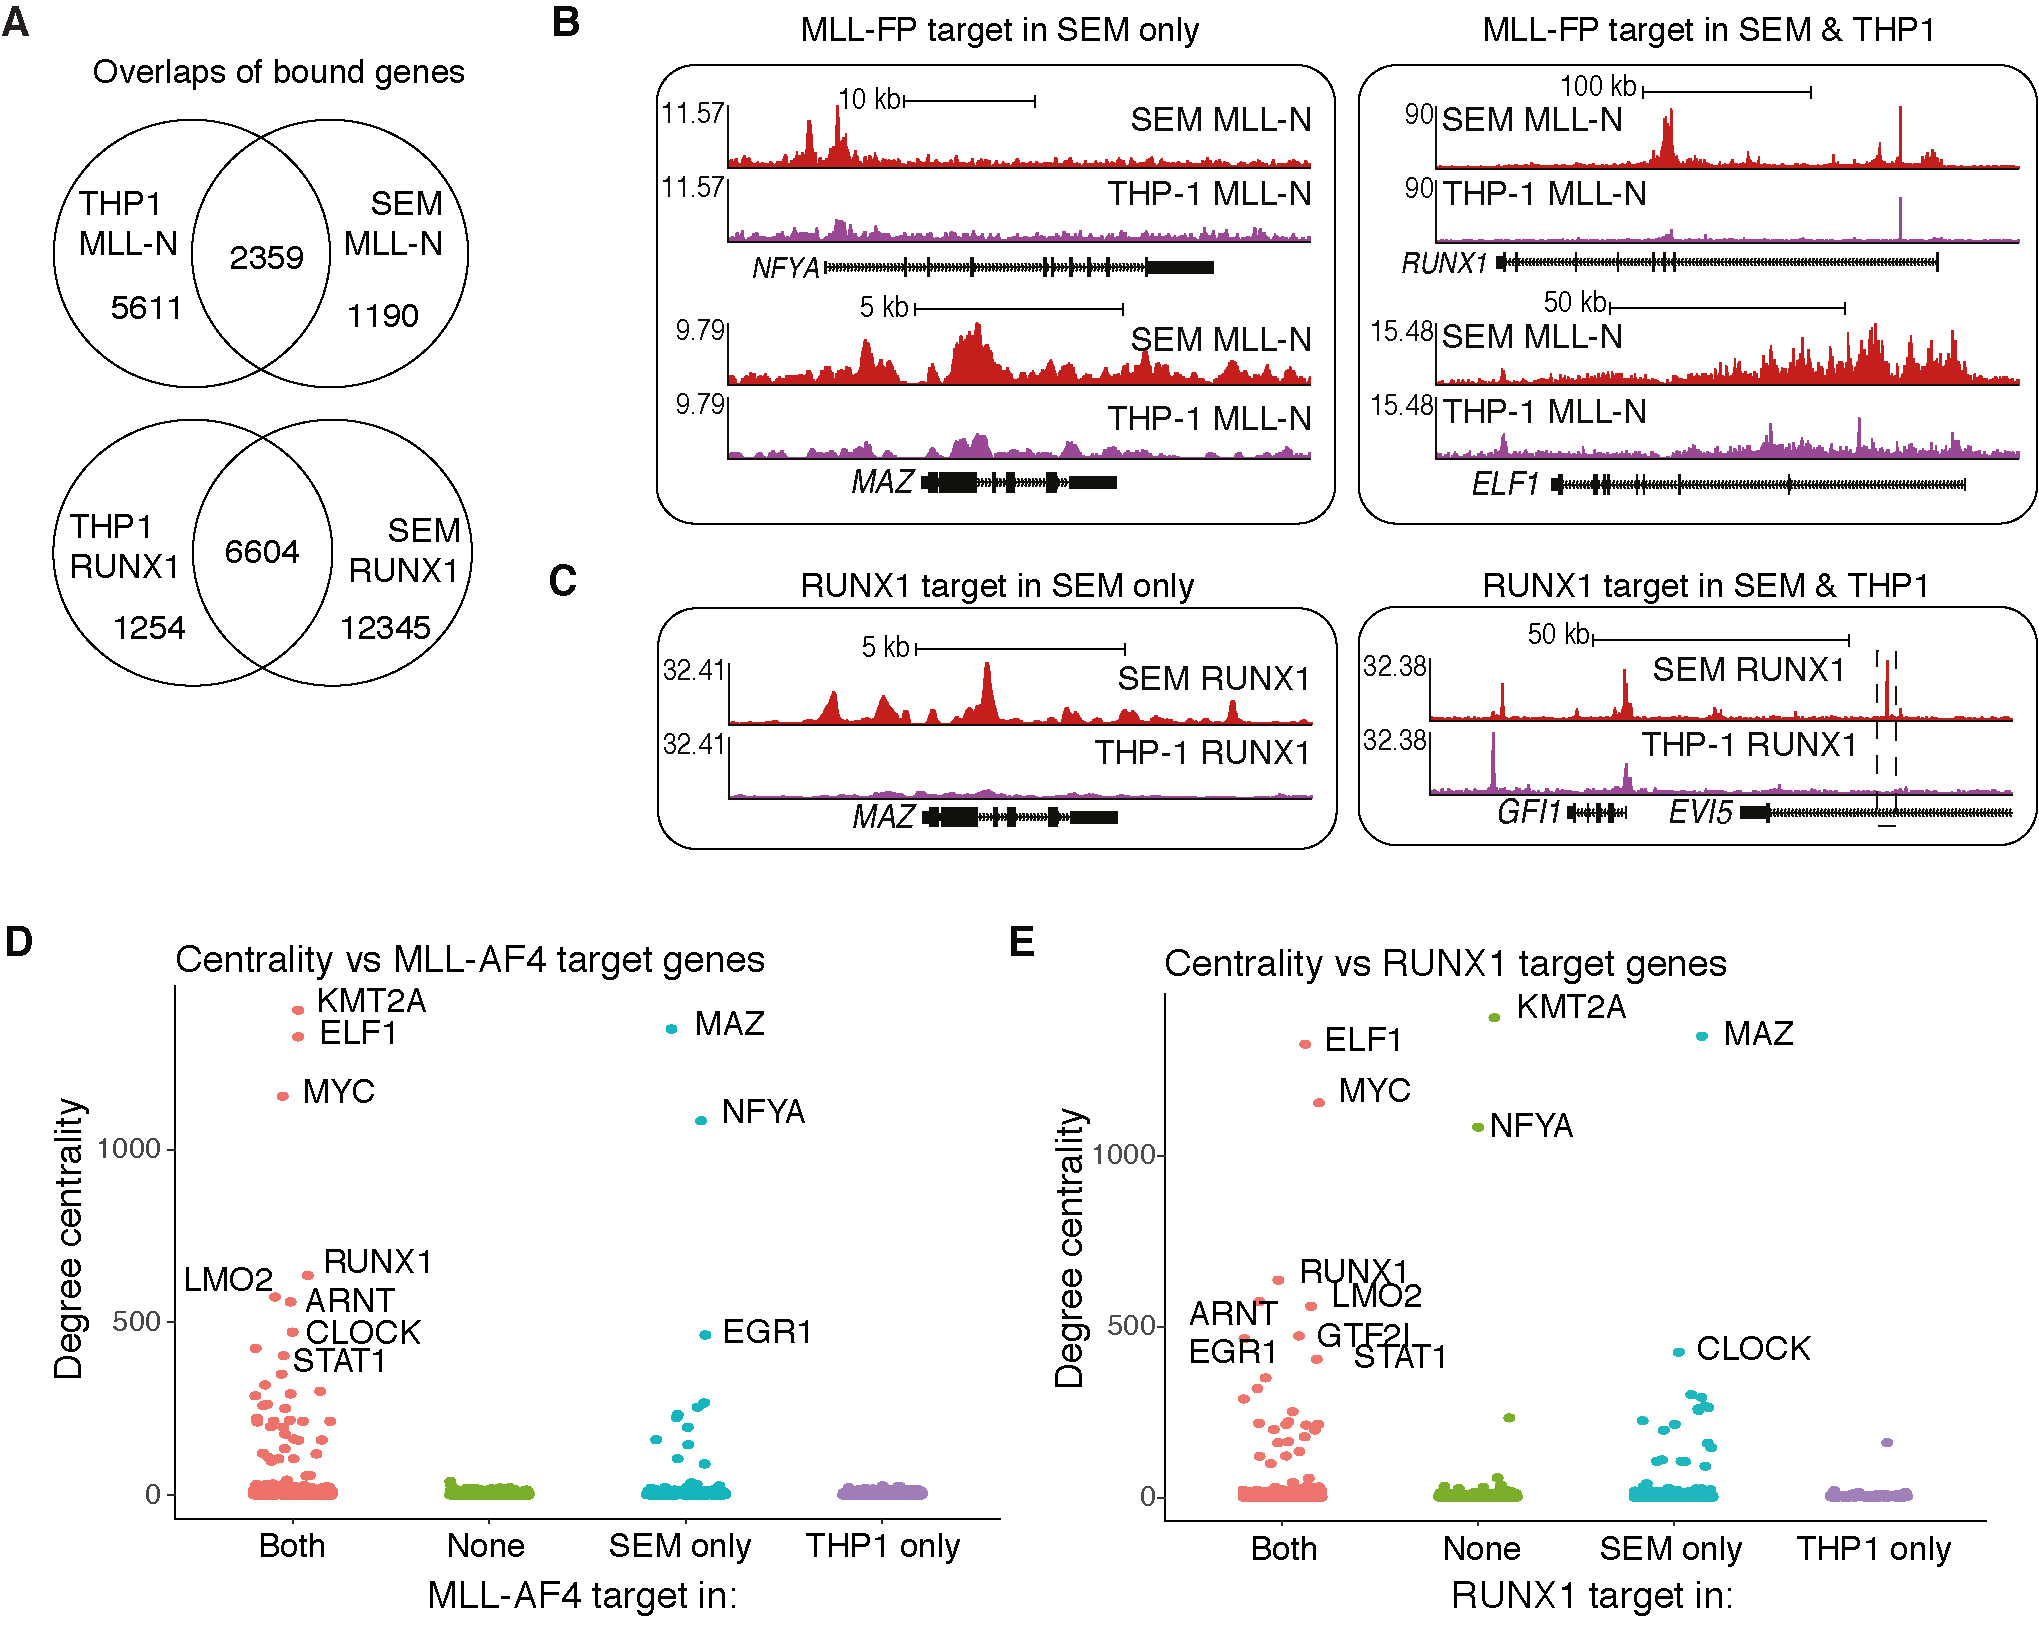
\includegraphics[width=\textwidth,height=\textheight,keepaspectratio]{figures/chapter4/ch4_sem-thp1.png}
    %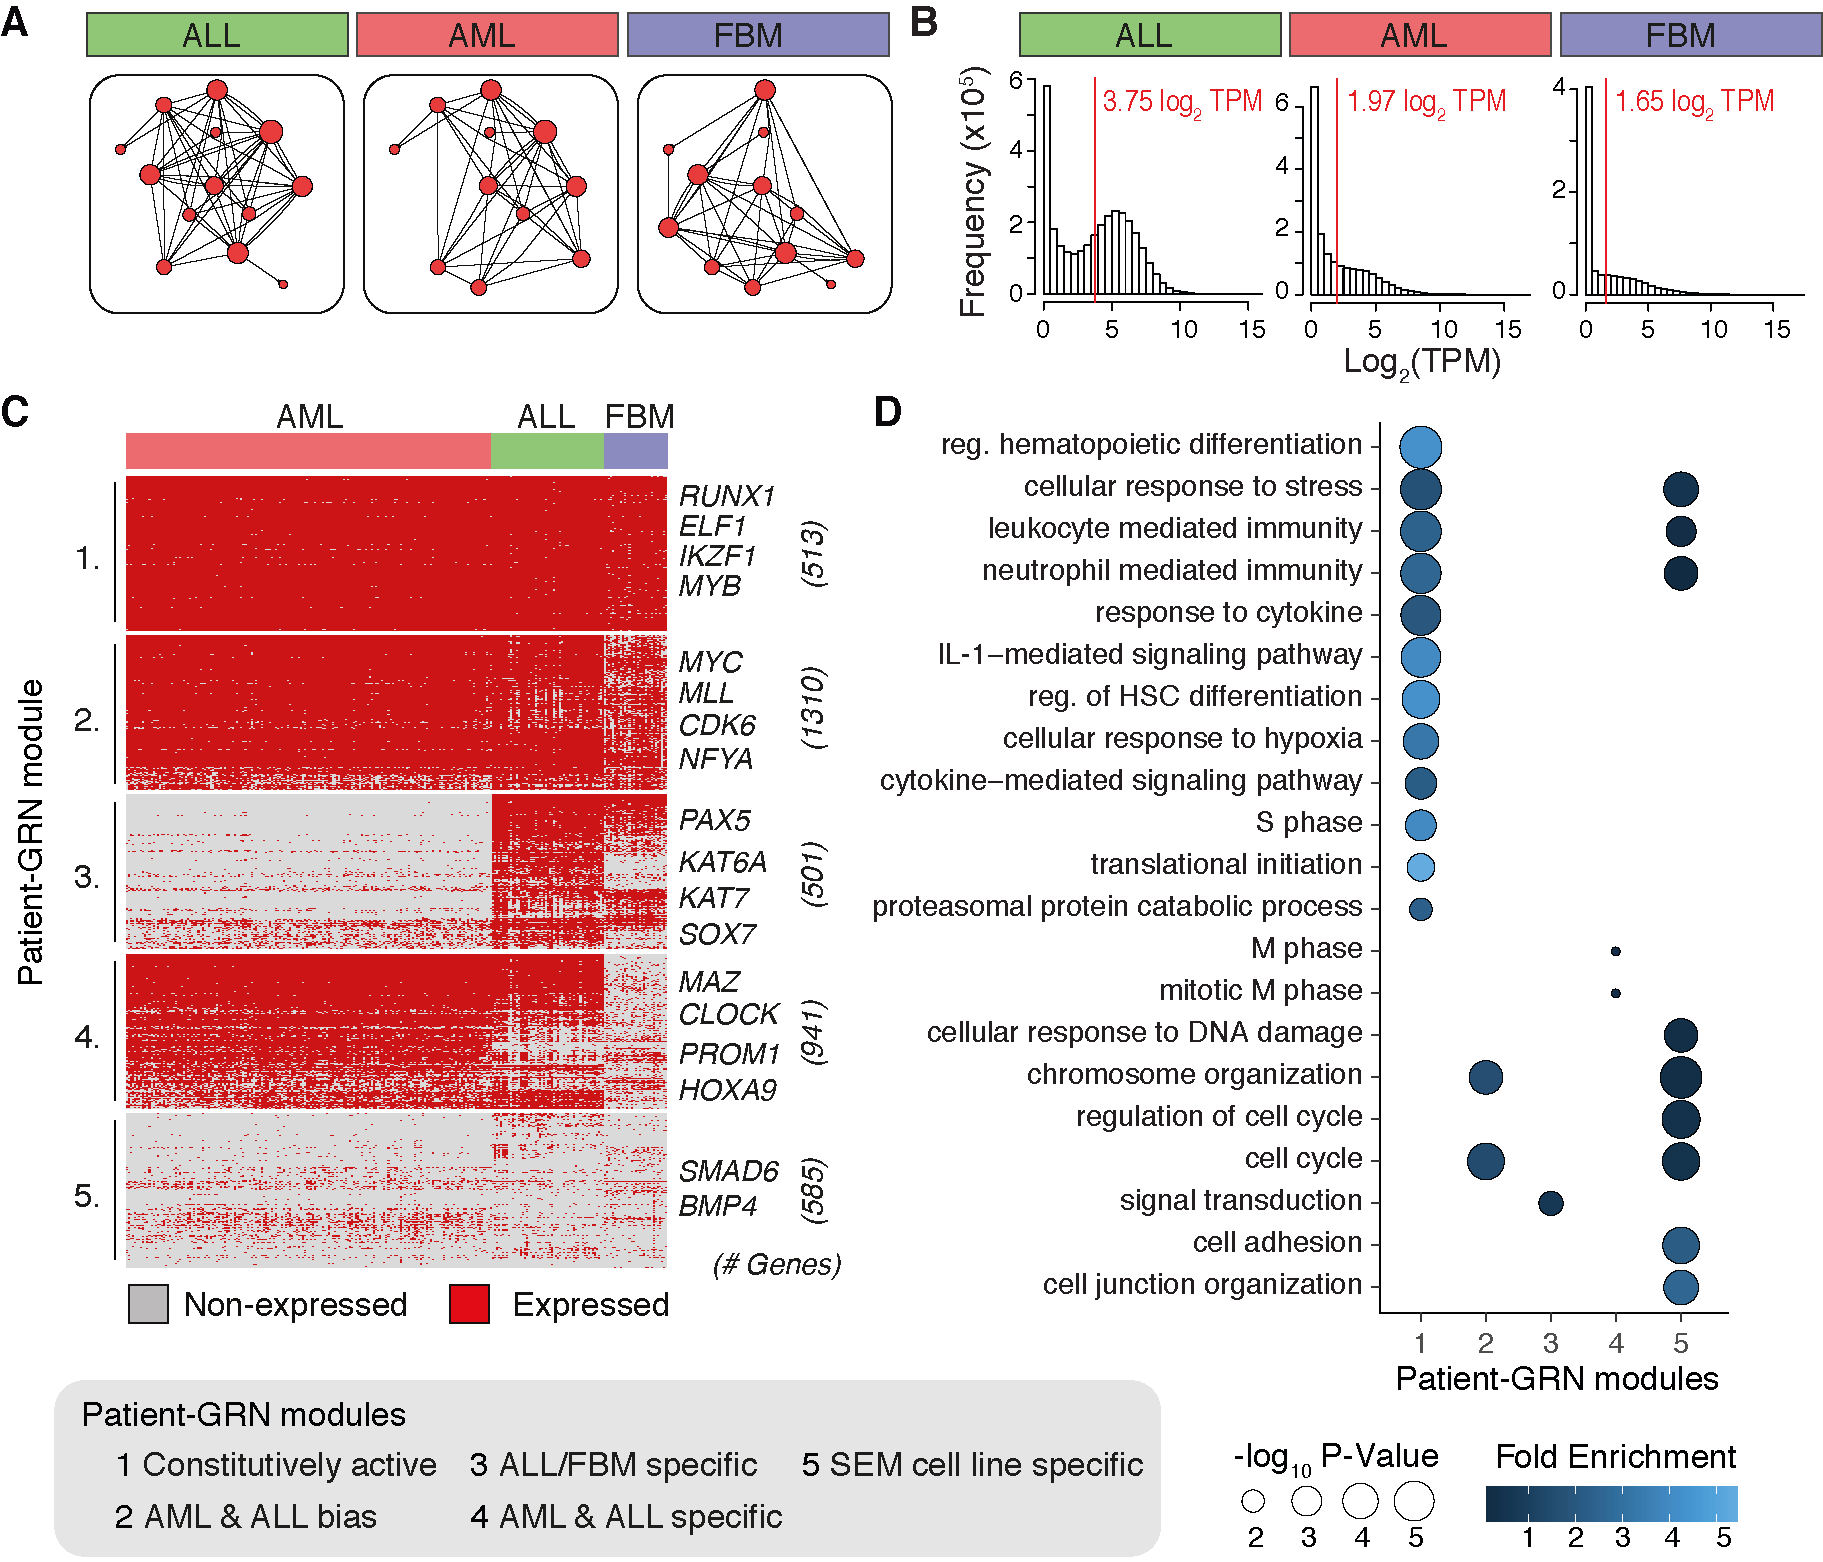
\includegraphics{figures/chapter4/ch4_patient.png}
    \caption[{The MLL-AF4 GRN predicts core interactions representative of both MLL-AF4 ALL and MLL-AF9 AML.}]
    {\textbf{The MLL-AF4 GRN predicts core interactions representative of both MLL-AF4 ALL and MLL-AF9 AML.} 
    \textbf{(A)} Overlaps of MLL-FP or RUNX1 bound genes in THP-1 and SEM cells. 
    \textbf{(B, C)} ChIP-seq tracks for MLL-N (B) and RUNX1 (C) in SEM and THP-1 cells. Dashed box highlights SEM specific RUNX1 peak.
    \textbf{(D, E)} Association of degree centrality with MLL-FP (D) or RUNX1 (E) bound gene overlaps in THP-1 and SEM cells as shown in (A). 
    \textit{Adapted from \cite{harman_kmt2a-aff1_2021}.}
    }
    \label{fig:ch4_sem-thp1}
\end{figure}

\section[Validating the importance of central regulatory hubs]{\label{ch4:key-hubs}Validating the importance of central\\regulatory hubs}

The analysis thus far builds a case for a core program common across \textit{MLL}r leukaemia, and implicates several TFs as key regulatory hubs based on degree centrality. Previous studies in \textit{S. cerevisiae}, \textit{C. elegans}, and \textit{D. melanogaster} have shown that multiple centrality measures are associated with essential proteins \citep{hahn_comparative_2005, jeong_lethality_2001, koschutzki_centrality_2008}. However, while important, many highly connected TFs in networks have overlapping roles, promoting robustness and suggesting multiple perturbations may be required to disrupt a process \citep{lehner_systematic_2006, byrne_global_2007, macneil_gene_2011}. As such, it is important to confirm that centrality measures can be used to determine important nodes, and estimate the nodes most susceptible to perturbation.

\subsection{\label{ch4:essential}Essentiality screens validate the importance of several central TFs}

\begin{figure}[!t]
    \centering
    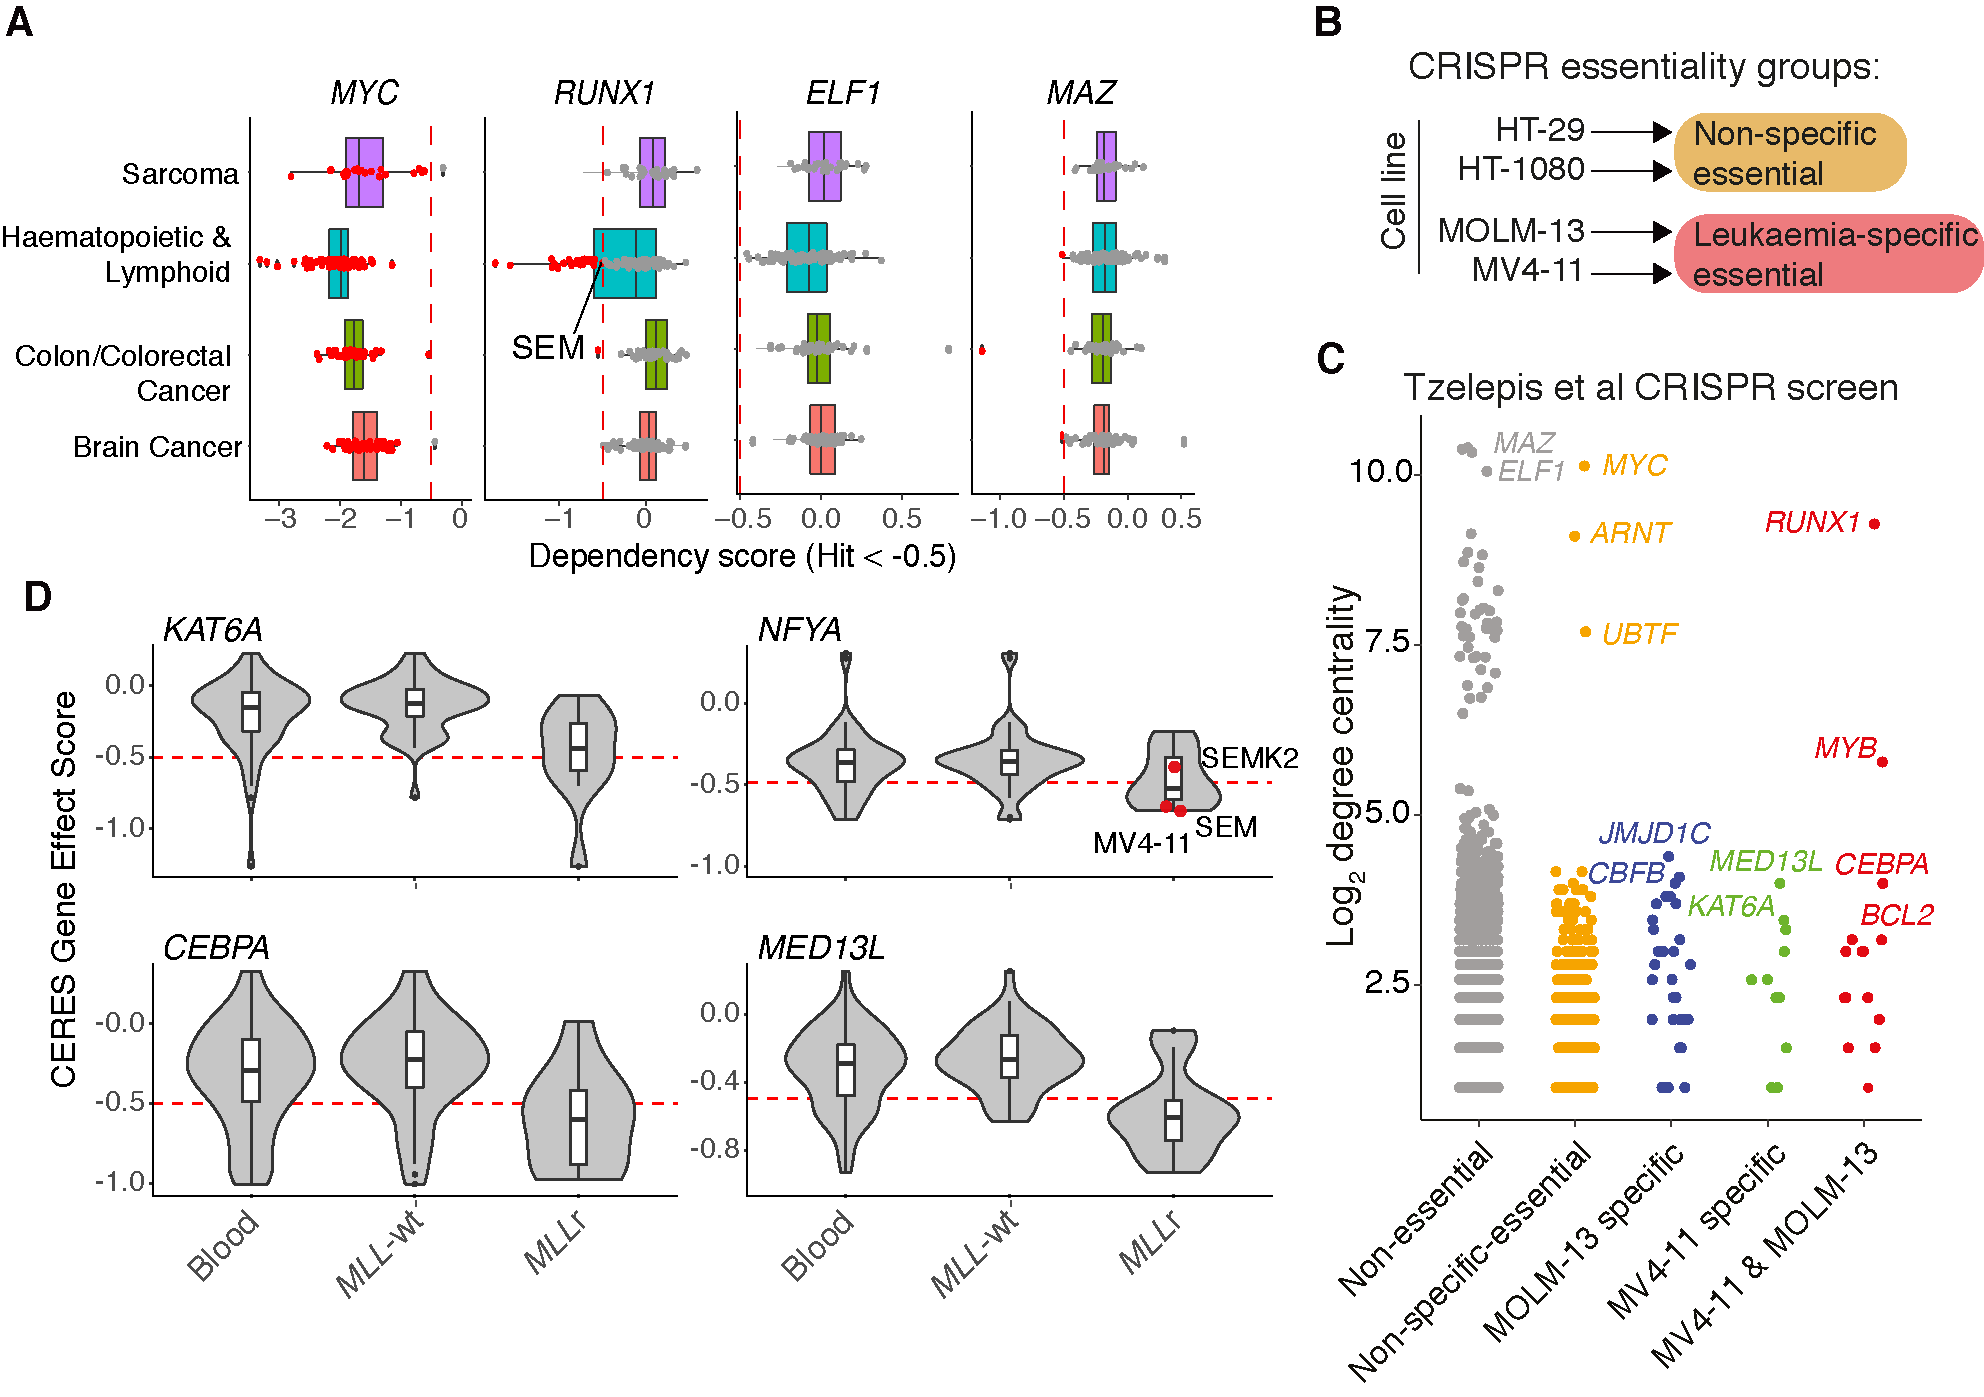
\includegraphics[width=\textwidth,height=\textheight,keepaspectratio]{figures/chapter4/ch4_essentiality.png}
    %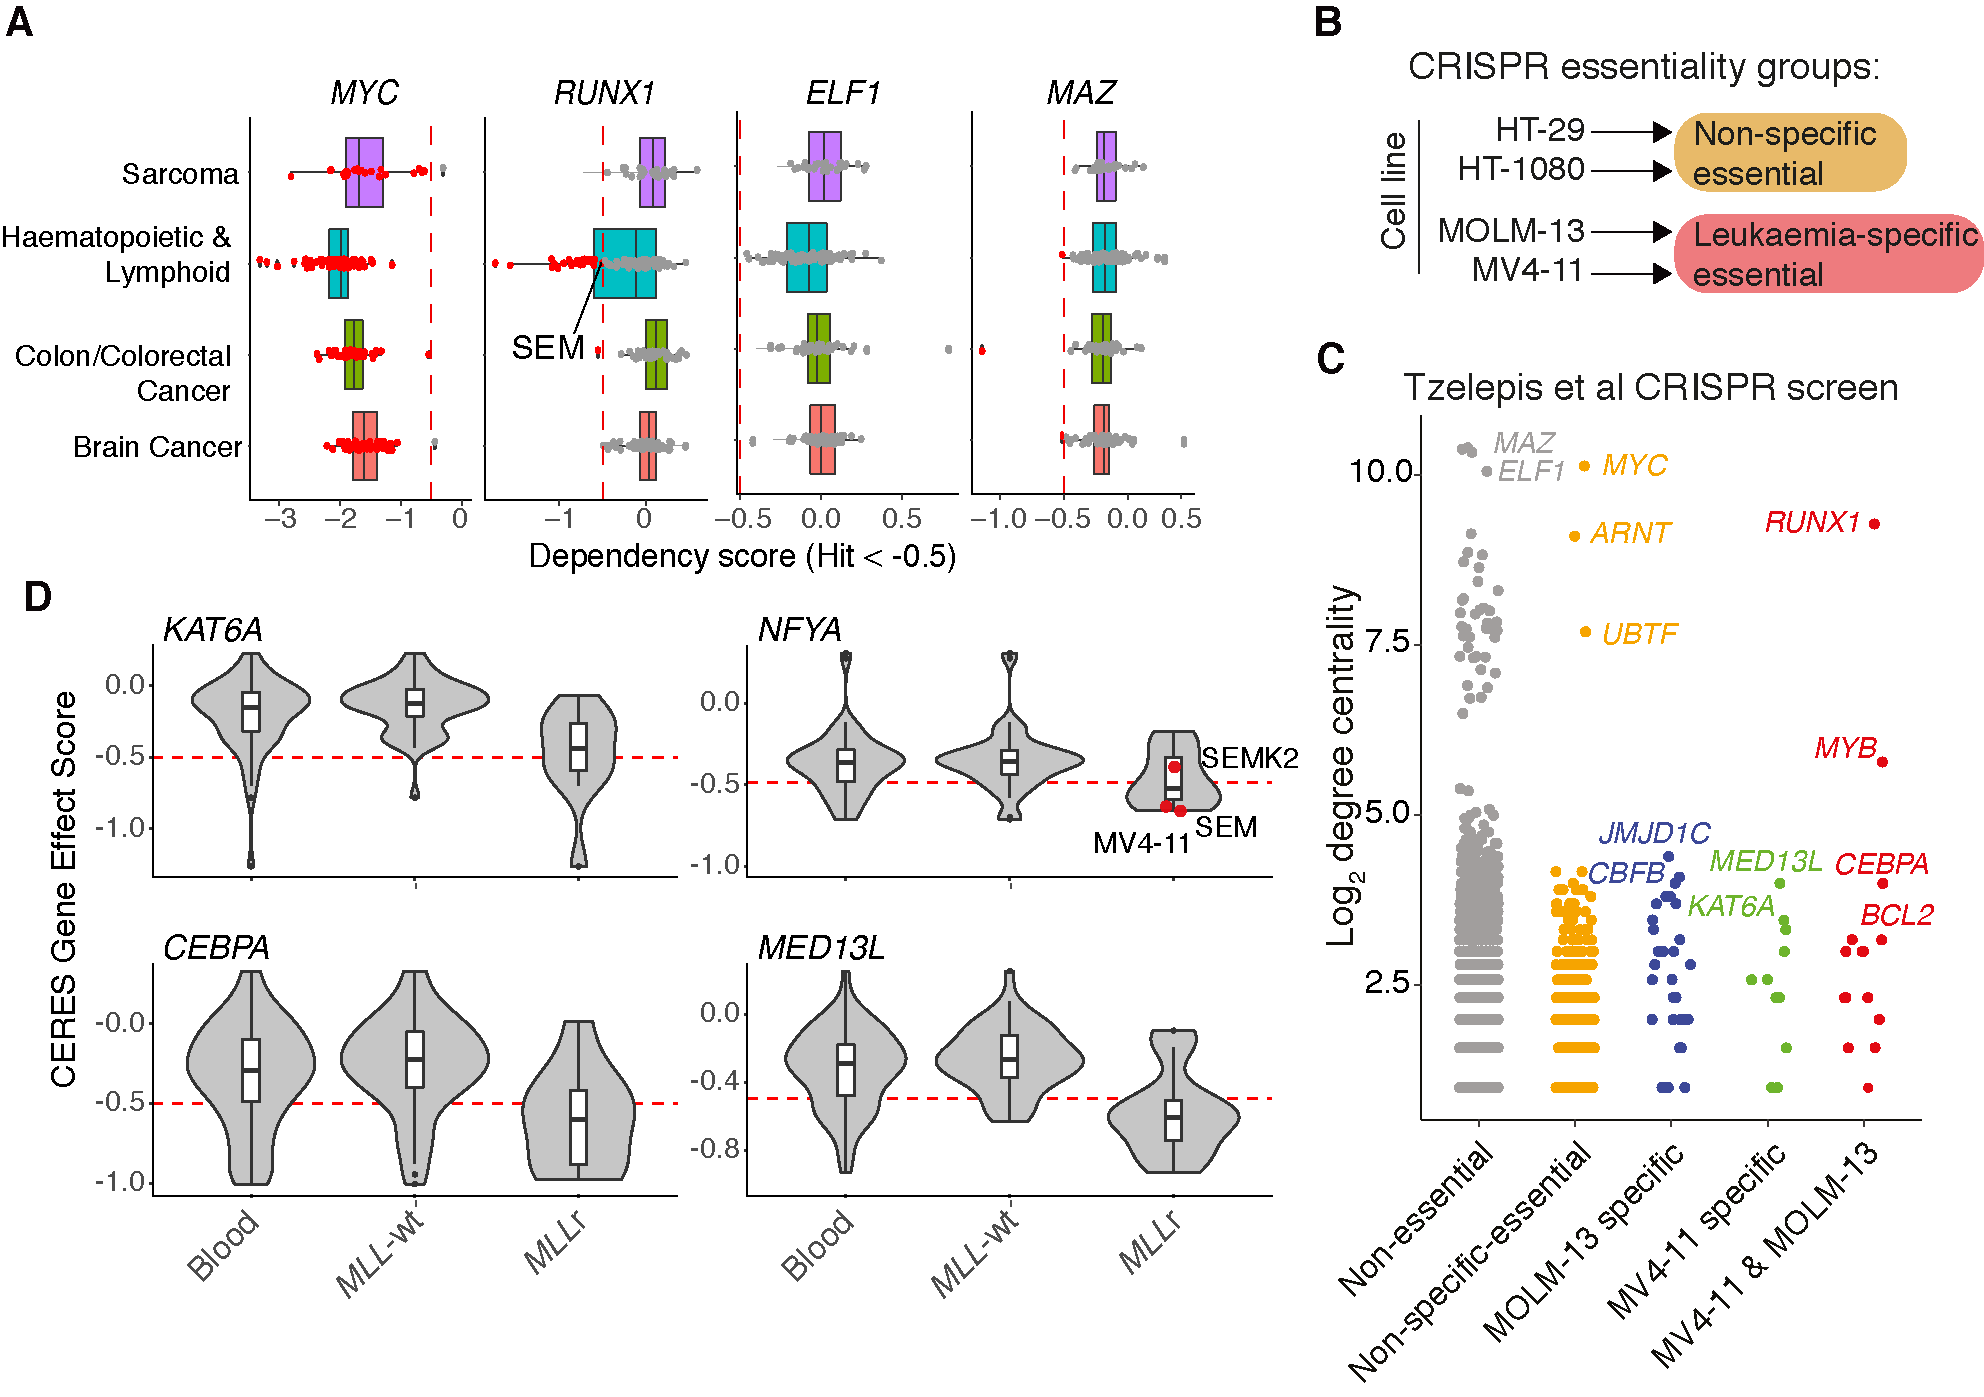
\includegraphics{figures/chapter4/ch4_essentiality.png}
    \caption[{Essential genes.}]
    {\textbf{CRISPR essentiality screens highlight RUNX1 as a critical central TF in MLL-FP leukaemias.} 
    \textbf{(A)} CRISPR essentiality CERES scores from DepMap (Avana 21Q1, \cite{meyers_computational_2017, doench_optimized_2016}). Genes are considered essential with a dependency score below -0.5. Each datapoint represents a different cell line, with essential hits highlighted red.
    \textbf{(B)} Illustration for how CRISPR essentiality screen hits from \cite{tzelepis_crispr_2016} are categorized. Essential genes in HT-29 or HT-1080 were "non-specific essential". Genes not essential in HT-29 or HT-1080 but essential in MOLM-13 or MV4-11 were specific to leukemia. 
    \textbf{(C)} Stratification of log\textsubscript{2} degree centrality (MLL-AF4 GRN) by CRISPR essentiality groups as outlined in B. 
    \textbf{(D)} CERES scores in haematopoietic cancer cell lines from DepMap, stratified by MLL translocation status. Red datapoints for \textit{NFYA} indicate MLL-AF4 cell lines. 
    \textit{Analysis in D performed by T. Wilson, supervised by me. CRISPR scores sourced from DepMap and \cite{tzelepis_crispr_2016}. Adapted from \cite{harman_kmt2a-aff1_2021}.} 
    }
    \label{fig:ch4_essentiality}
\end{figure}

To validate whether central TFs are important for leukaemogenesis, I integrated publicly available CRISPR essentiality screens. The Cancer Dependency Map (DepMap, Avana 21Q1 dataset, \cite{meyers_computational_2017, doench_optimized_2016}) found \textit{MYC} to be pan-essential, \textit{RUNX1} to be essential in multiple haematopoietic cancer models, and \textit{ELF1} and \textit{MAZ} to be non-essential (Fig. \ref{fig:ch4_essentiality}A). As this is a large and generalised screen, I integrated a more targeted screen from \cite{tzelepis_crispr_2016} which includes two \textit{MLL}r cell lines, MOLM-13 (MLL-AF9 AML) and MV4-11 (MLL-AF4 AML), alongside two non-leukaemic cancer cell lines, HT-29 (colon adenocarcinoma) and HT-1080 (fibrosarcoma). To find genes essential specifically in leukaemia, hits were categorised as non-essential, non-specific essential (hit in HT-29 or HT-1080), or essential in one or both \textit{MLL}r leukaemias (hit in MOLM-13 and/or MV4-11, but not HT-29 or HT-1080) (Fig. \ref{fig:ch4_essentiality}B-C). In line with the DepMap data, \textit{MYC} was pan-essential, while \textit{MAZ} and \textit{ELF1} were not essential in any cell line. This suggests \textit{MAZ} and \textit{ELF1}, while highly connected, are not important for survival or proliferation, at least in AML. \textit{RUNX1} was essential in both MOLM-13 and MV4-11 cells, highlighting its importance under the control of both MLL-AF4 and -AF9 fusion proteins. Other central leukaemia-specific hits include \textit{MYB}, \textit{MED13L}, \textit{CEBPA}, and \textit{KAT6A} (Fig. \ref{fig:ch4_essentiality}C). 

The MV4-11 and MOLM-13 essential gene \textit{CEBPA}, along with the MV4-11 specific hits \textit{MED13L} and \textit{KAT6A}, show greater essentiality for \textit{MLL}r samples over non-\textit{MLL}r blood cancers (Fig. \ref{fig:ch4_essentiality}D). NF-YA is a central (but not core to all MLL-FPs) node in the GRN and is not significantly essential in the \cite{tzelepis_crispr_2016} screen. However, the DepMap screen shows higher essentiality for NF-YA in \textit{MLL}r samples, with \textit{MLL-AF4} cell lines (SEM and MV4-11) showing the high essentiality (Fig. \ref{fig:ch4_essentiality}D). This indicates that not only are these genes essential for MLL\textit{r} AML, but show generally greater essentiality for \textit{MLL}r leukaemias than other haematopoietic malignancies, possibly in part as a core-program targeted by all MLL-FPs. Overall, this analysis shows that degree centrality highlights many essential genes, and identifying high centrality in TFs critical for both MLL-AF4 and MLL-AF9 AML.

\subsection{\label{ch4:stress-centrality}Stress is a better indicator of essentiality than degree centrality}

As demonstrated, while degree centrality highlights nodes that regulate a wide range of targets and are often critical, this measure does not always translate into essentiality for leukaemic cells. Stress centrality (a variant of betweenness centrality) may better reflect essentiality, as it represents nodes less likely to be compensated for upon perturbation (see introduction section \ref{ch1:centrality}, p.\pageref{ch1:centrality}, Fig. \ref{fig:ch1_stress-example}). In fact, while there is a slight enrichment in degree centrality for MV4-11 essential genes, there is much higher stress centrality observed in MV4-11 essential genes over non-essential genes (Fig. \ref{fig:ch4_centrality}A). \textit{MAZ} was a non-essential TF, which despite high connectivity, shows relatively low stress centrality than comparably connected TFs (Fig. \ref{fig:ch4_centrality}B). Exploring the ratio between stress and degree centrality, RUNX1 has a far higher stress for its connectivity than other TFs (degree 636, stress 80864), and while MYB is not highly connected it also shows a very high stress:degree ratio (degree 56, stress 3797) (Fig. \ref{fig:ch4_centrality}C). It has been suggested that nodes with low degree and high stress are particularly important factors for connecting network modules \citep{joy_high-betweenness_2005, koschutzki_centrality_2008}, placing RUNX1 as a critical TF in bridging interactions between factors, such as MLL-AF4.

\begin{figure}[!t]
    \centering
    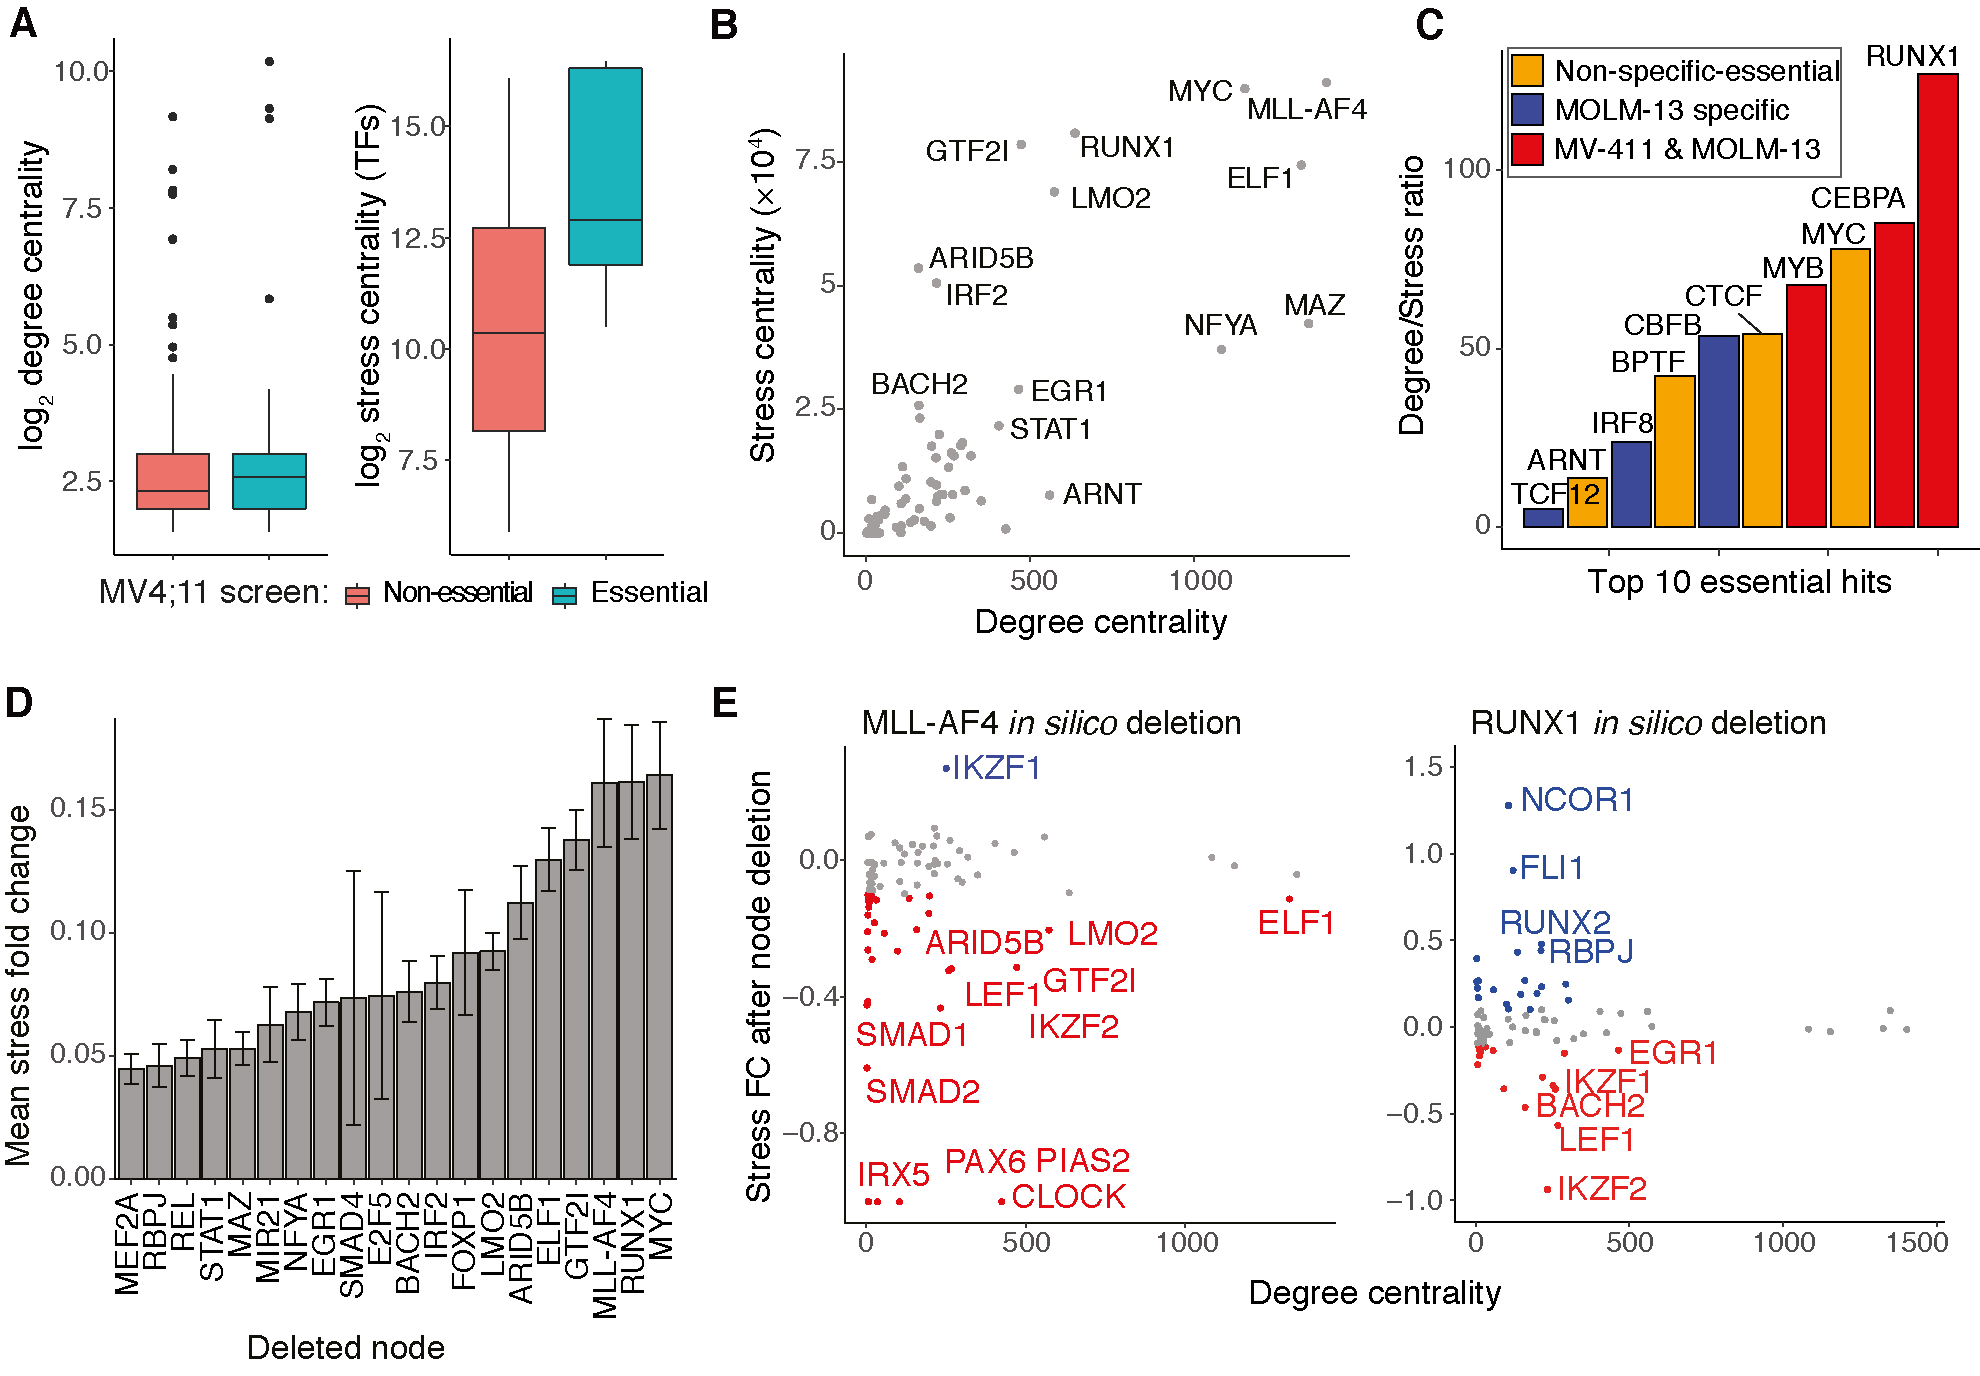
\includegraphics[width=\textwidth,height=\textheight,keepaspectratio]{figures/chapter4/ch4_centrality.png}
    %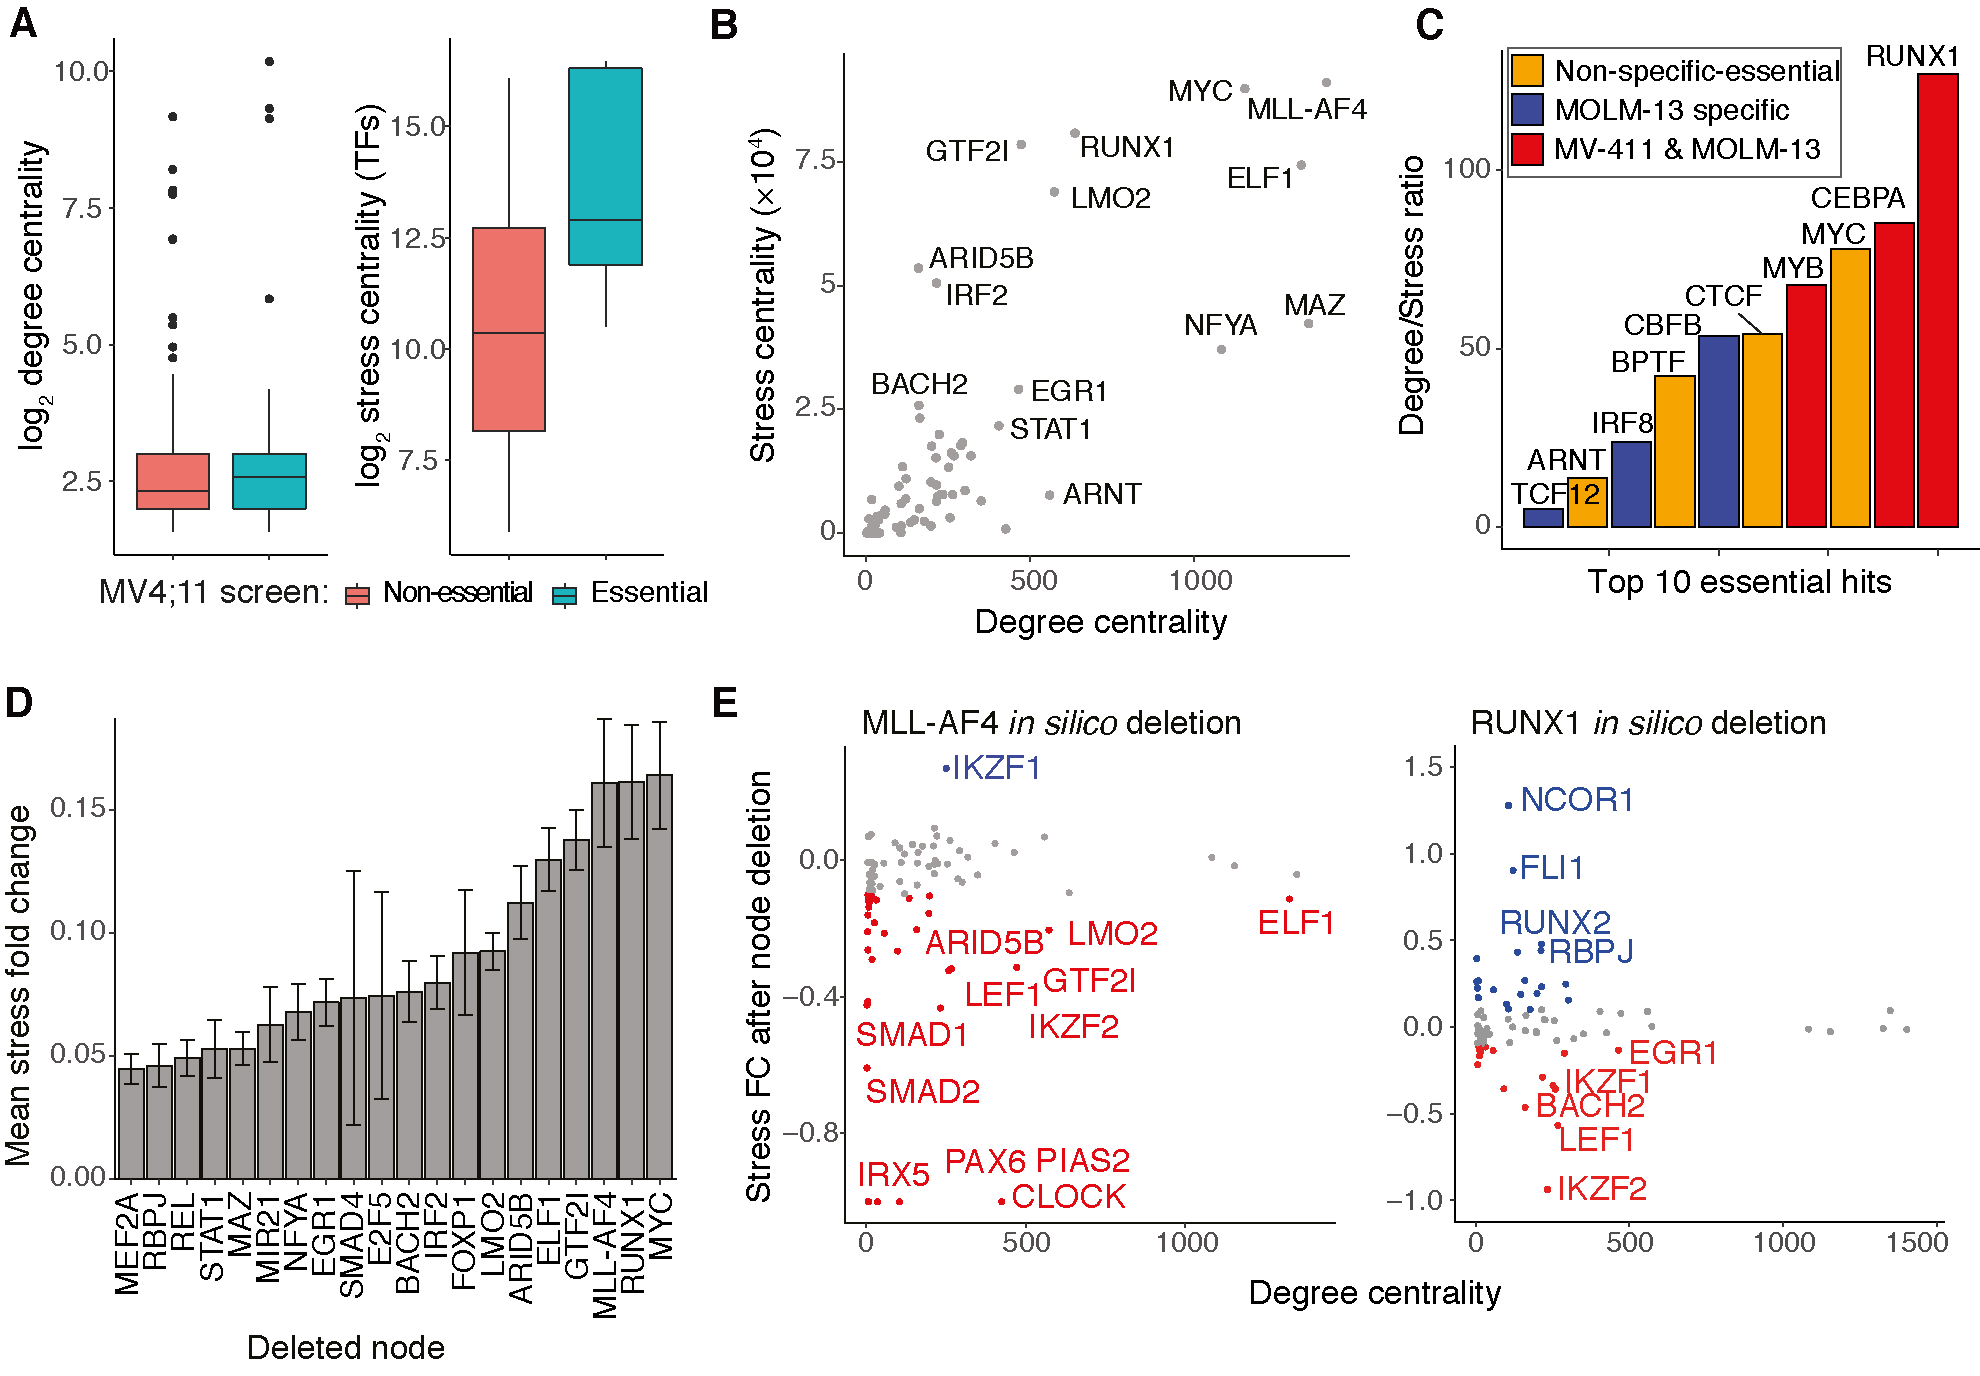
\includegraphics{figures/chapter4/ch4_centrality.png}
    \caption[{Centrality analysis of MLL-AF4 GRN.}]
    {\textbf{Centrality analysis of MLL-AF4 GRN.} 
    \textbf{(A)} Log\textsubscript{2} degree and stress centrality of the MLL-AF4 GRN nodes plotted by MV4-11 essentiality from \cite{tzelepis_crispr_2016}. 
    \textbf{(B)} Relationship between degree and stress centrality of MLL-AF4 GRN nodes. 
    \textbf{(C)} Rank order plot of ratios between stress and degree centrality for ten most essential GRN hubs from \cite{tzelepis_crispr_2016}. 
    \textbf{(D)} Top 20 in silico deleted nodes by mean stress FC (methods section \ref{ch2:centrality}, p.\pageref{ch2:centrality}). 
    \textbf{(E)} Stress FC after in silico deletion of RUNX1 or MLL-AF4, plotted against degree centrality. Blue and red indicate positive (FC > 0.1) and negative (FC < -0.1) stress FC, respectively. 
    \textit{Adapted from \cite{harman_kmt2a-aff1_2021}.}
    }
    \label{fig:ch4_centrality}
\end{figure}

As discussed, central TFs may contain redundant regulatory logic that compensates for specific perturbation. To investigate alternative nodes that may facilitate TF compensation, I established an approach where each GRN node was deleted in silico, and stress centrality values recalculated. Stress values before and after in silico deletion were compared as stress fold change (stress FC), and summarised for every node (Fig. \ref{fig:ch4_centrality}D). RUNX1 and MYC in silico deletion showed the greatest stress redistribution, above MLL-AF4, while the non-essential factors MAZ and NFYA show less stress FC redistribution (Fig. \ref{fig:ch4_centrality}D). Looking in detail, MLL-AF4 deletion results in negative stress FC while RUNX1 shows positive and negative stress FC. RUNX1 in silico deletion shows increased NCOR1, FLI1, RBPJ and RUNX2 stress, while factors such as IKZF1 and IKZF2 are reduced (Fig. \ref{fig:ch4_centrality}E), indicating that these TFs provide an alternative route to reach RUNX1 target nodes. RUNX2 is expected as it shares the RUNT domain with RUNX1, and therefore can likely compensate for perturbation. RUNX1 has been shown to cooperate with FLI1, altering its binding affinity for the FLI1 motif and remodelling FLI1 regulatory logic \citep{gilmour_co-operation_2018, lichtinger_runx1_2012}. RBPJ is a transcriptional repressor, yet forms a transactivating complex with NOTCH intracellular domain (NICD) \citep{kojika_notch_2001}. RUNX1 and RBPJ-NICD cooperate at specific loci, for example to coregulate the +1.27 Mb \textit{MYC} enhancer and \textit{IL7R} enhancers \citep{choi_runx1_2017, wang_notch1-rbpj_2014}. This cooperative behaviour is indicative of shared regulatory logic, and while these factors function in combination, it is likely they regulate common sites in the absence of RUNX1. Genes that decrease in stress may reflect a breakdown in network pathways. For example, if node pairs must communicate through a RUNX1:IKZF1 axis then loss of RUNX1 will break down the path of communication via IKZF1. This places IKZF1 as a key target of RUNX1, required for downstream communication within the network. This lines up with Runx1 regulation of Ikzf1 in EHT, which was predicted to enact TF cascades to repress Notch genes (Fig. \ref{fig:ch3_runx1-ikzf1-notch}D, p.\pageref{fig:ch3_runx1-ikzf1-notch}). This analysis serves to rank nodes based on stress centrality, which may better reflect importance, and predicts compensatory mechanisms upon perturbation. In particular it highlights RUNX1, MYB, CEBPA and MYC as highly important TFs, and notes potential redundancy between RUNX1 and specific factors at a subset of targets. 

\section{\label{ch4:mll-af4-runx1}MLL-AF4 and RUNX1 cooperate to regulate gene expression}

\subsection{Generating, and characterising a RUNX1 driven GRN model of leukaemia}

\begin{figure}[!b]
    \centering
    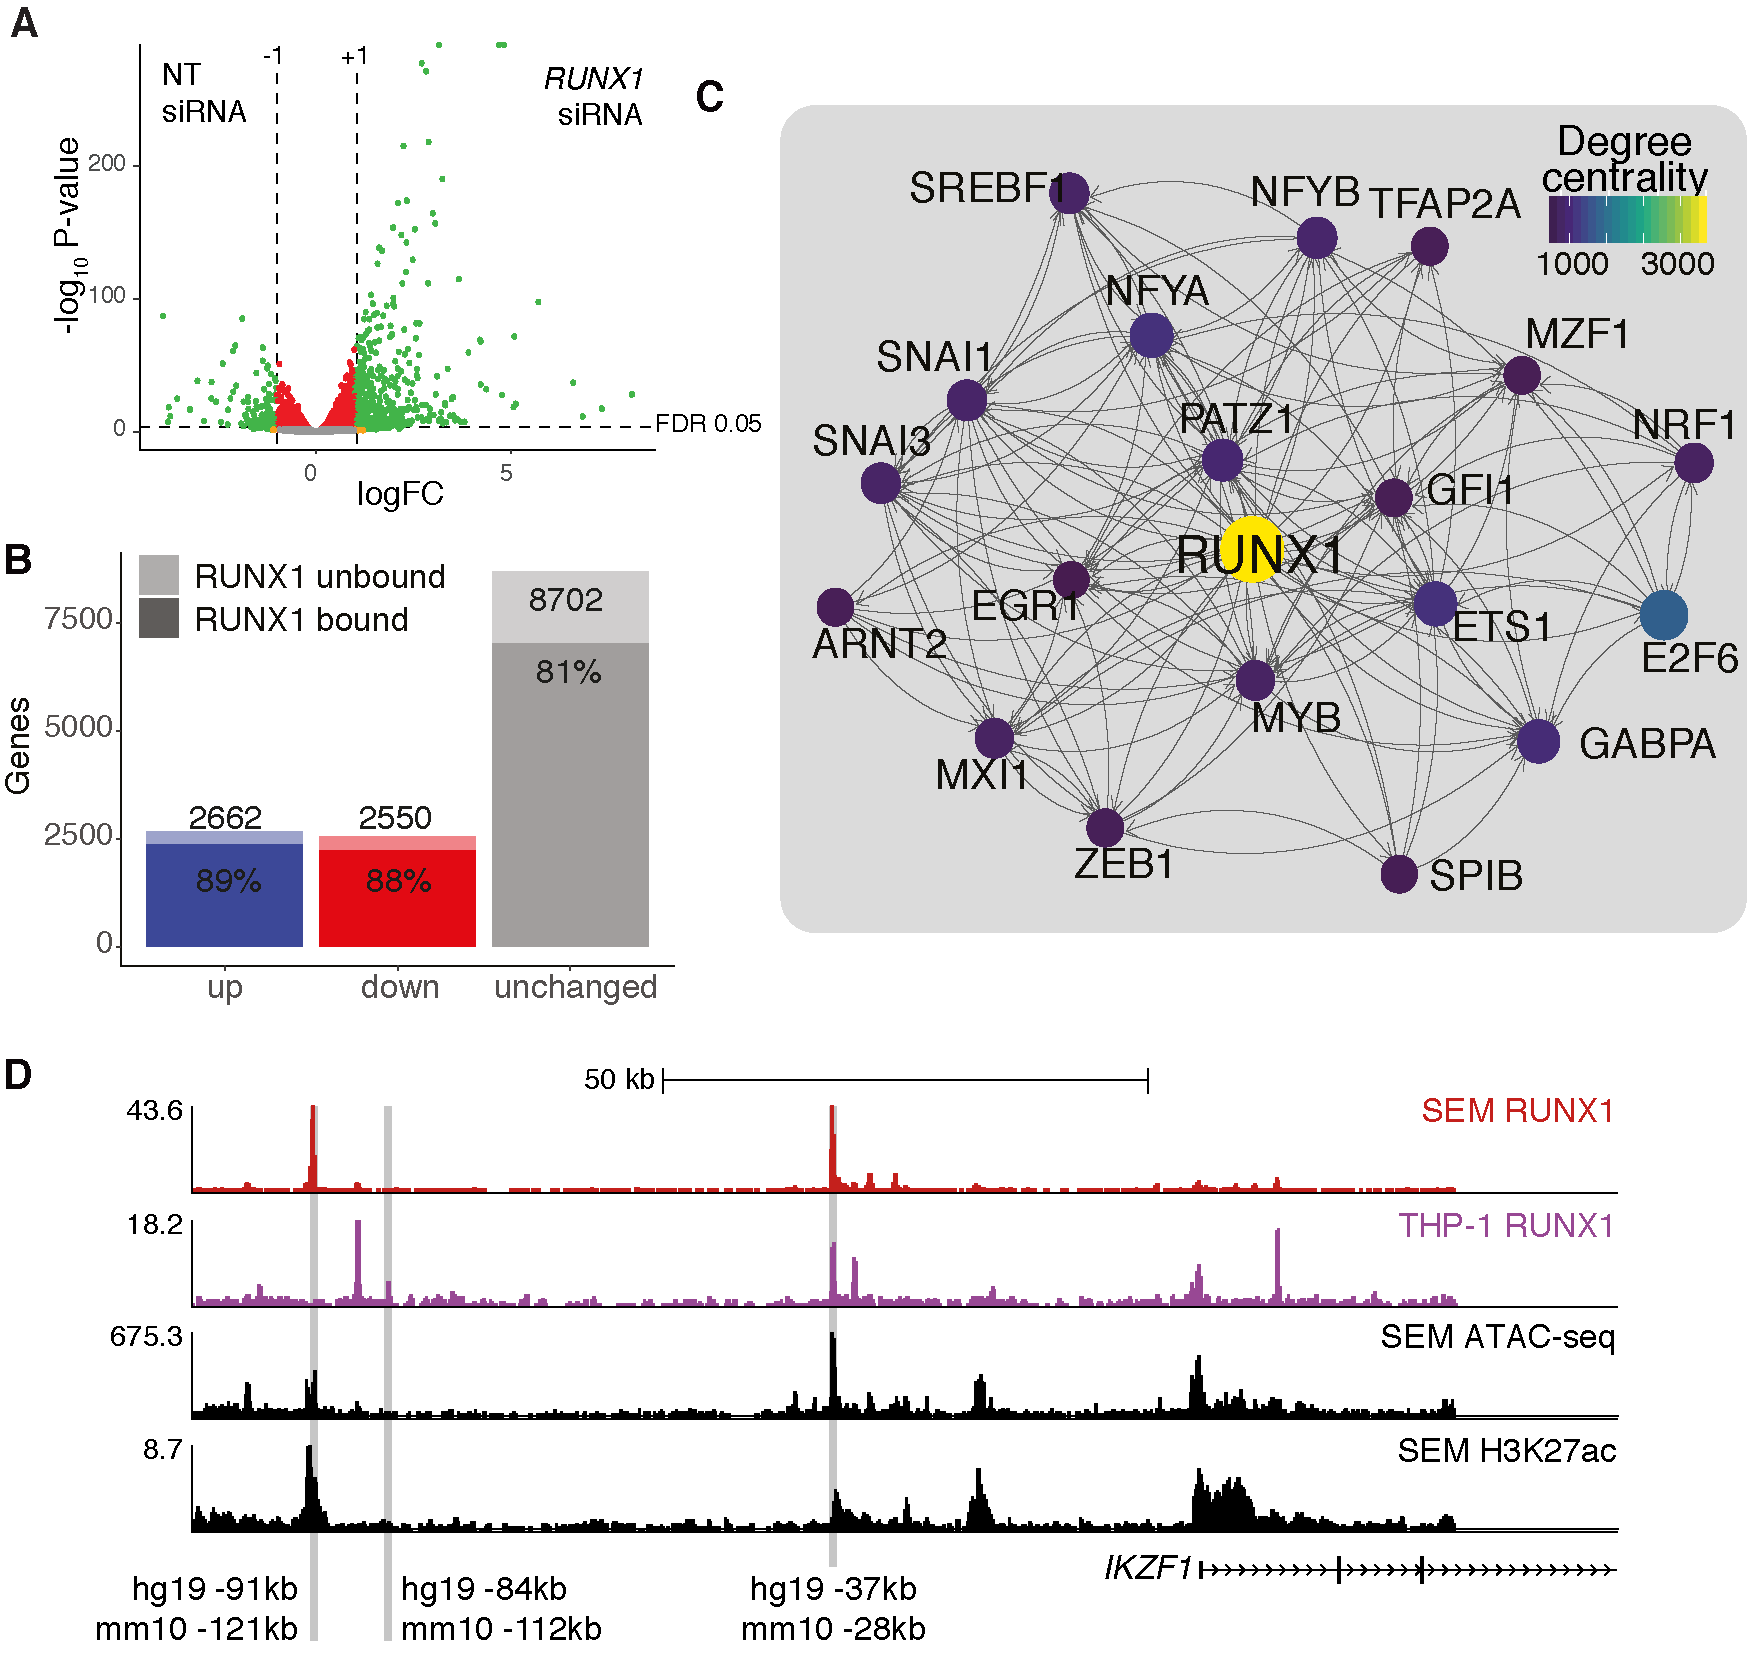
\includegraphics[width=\textwidth,height=\textheight,keepaspectratio]{figures/chapter4/chr4_runx1-grn.png}
    %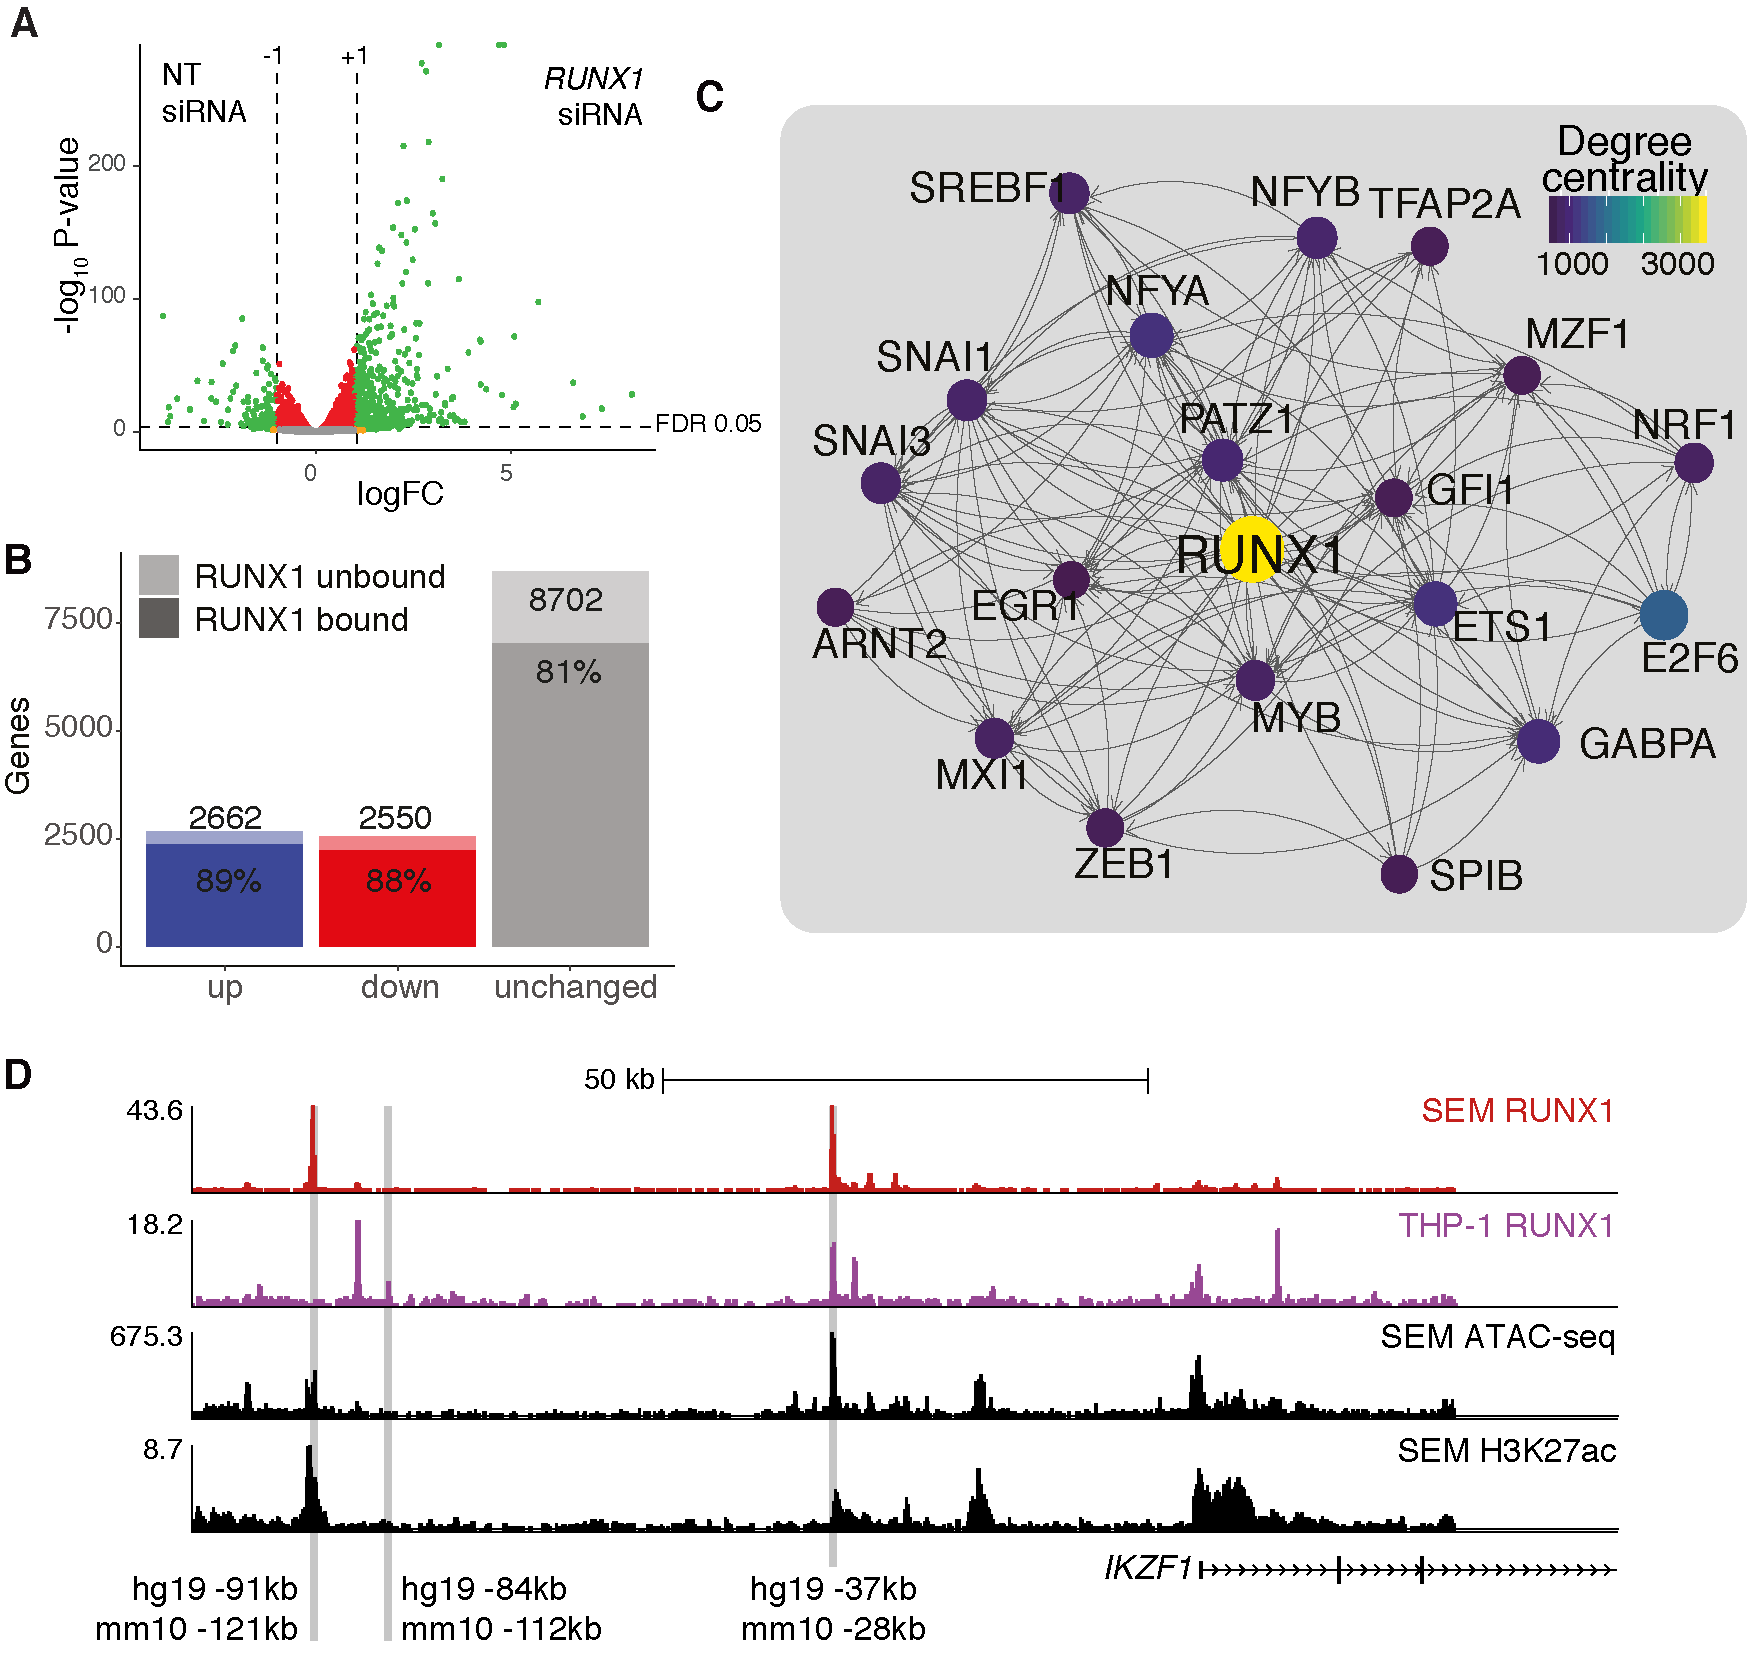
\includegraphics{figures/chapter4/chr4_runx1-grn.png}
    \caption[{Establishing a RUNX1 centred GRN in SEM cells.}]
    {\textbf{Establishing a RUNX1 centred GRN in SEM cells.} 
    \textbf{(A)} Relationship between -log\textsubscript{10} P value and logFC in \textit{RUNX1} KD nascent RNA-seq. Genes are coloured by logFC and FDR thresholds as indicated by dashed lines.
    \textbf{(B)} DEGs from nascent RNA-seq after 96 h \textit{RUNX1} KD (\textit{n} = 3). Shaded bar represents RUNX1-bound genes.
    \textbf{(C)} The top 20 genes of the RUNX1 GRN by degree centrality. Lines indicate predicted interaction from protein to gene locus, with arrowheads pointing downstream. 
    \textbf{(D)} ChIP-seq and ATAC-seq tracks at the human \textit{IKZF1} locus. Mouse -28, -112, and -121 enhancers are highlighted, matched by sequence similarity using UCSC BLAT. 
    \textit{Raw nascent RNA-seq data was generated by M. Tapia (Milne lab) and analysed by me. Adapted from \cite{harman_kmt2a-aff1_2021}.}
    } 
    \label{fig:ch4_runx1-grn}
\end{figure}

To begin to address how MLL-AF4 regulates a wider network in combination with TFs, I selected RUNX1 as an example of a critical MLL-AF4 activated node. Across multiple analyses RUNX1 was promoted as a critical TF within the MLL-AF4 GRN, it is highly central and is a core-TF active in both MLL-AF4 ALL and MLL-AF9 AML. To understand RUNX1 regulatory logic in detail, I established a RUNX1-centred GRN. Nascent RNA-seq data following 96 hours' \textit{RUNX1} KD generated by M. Tapia revealed 5212 DEGs, the majority of which were bound by RUNX1 (Fig. \ref{fig:ch4_runx1-grn}A-B). A RUNX1-centric GRN was established using this nascent RNA-seq and previously published RUNX1 ChIP-seq \citep{wilkinson_runx1_2013}, using the same approach as in Fig. \ref{fig:ch4_ma4-grn}. Many known targets of RUNX1, such as \textit{GFI1} \citep{wilson_gfi1_2010} and \textit{MYB} \citep{choi_runx1_2017}, were central to the RUNX1 GRN (Fig. \ref{fig:ch4_runx1-grn}C). A number of Runx1 targets in the EHT GRN (see section \ref{ch3:runx1-targets}, p.\pageref{ch3:runx1-targets}) are also present here, including, among others, \textit{MYB}, \textit{IKZF1/2}, \textit{SNAI1/3}, \textit{ZEB1/2}, \textit{GFI1} and the NOTCH targets \textit{HES1}, \textit{HEY1} and \textit{HEY2}. I compared RUNX1 binding at the \textit{IKZF1} locus with the EHT GRN and the mouse predicted enhancer elements (Fig. \ref{fig:ch3_runx1-ikzf1}, p.\pageref{fig:ch3_runx1-ikzf1}). RUNX1 binding at \textit{IKZF1} shows similar occupancy of the -28 and -121 enhancer elements (-37 kb and -91 kb in human) as in EHT, though the -112 enhancer (-84 kb in human) is not bound by RUNX1 (Fig. \ref{fig:ch4_runx1-grn}D). This suggests both GRN models capture common RUNX1 regulatory logic, though with some differences in enhancer occupancy, that is preserved across species and between different cell contexts.

\subsection[RUNX1 and MLL-AF4 GRNs intersect at leukaemogenic processes]{RUNX1 and MLL-AF4 GRNs intersect at\\leukaemogenic processes}

\begin{figure}[!t]
    \centering
    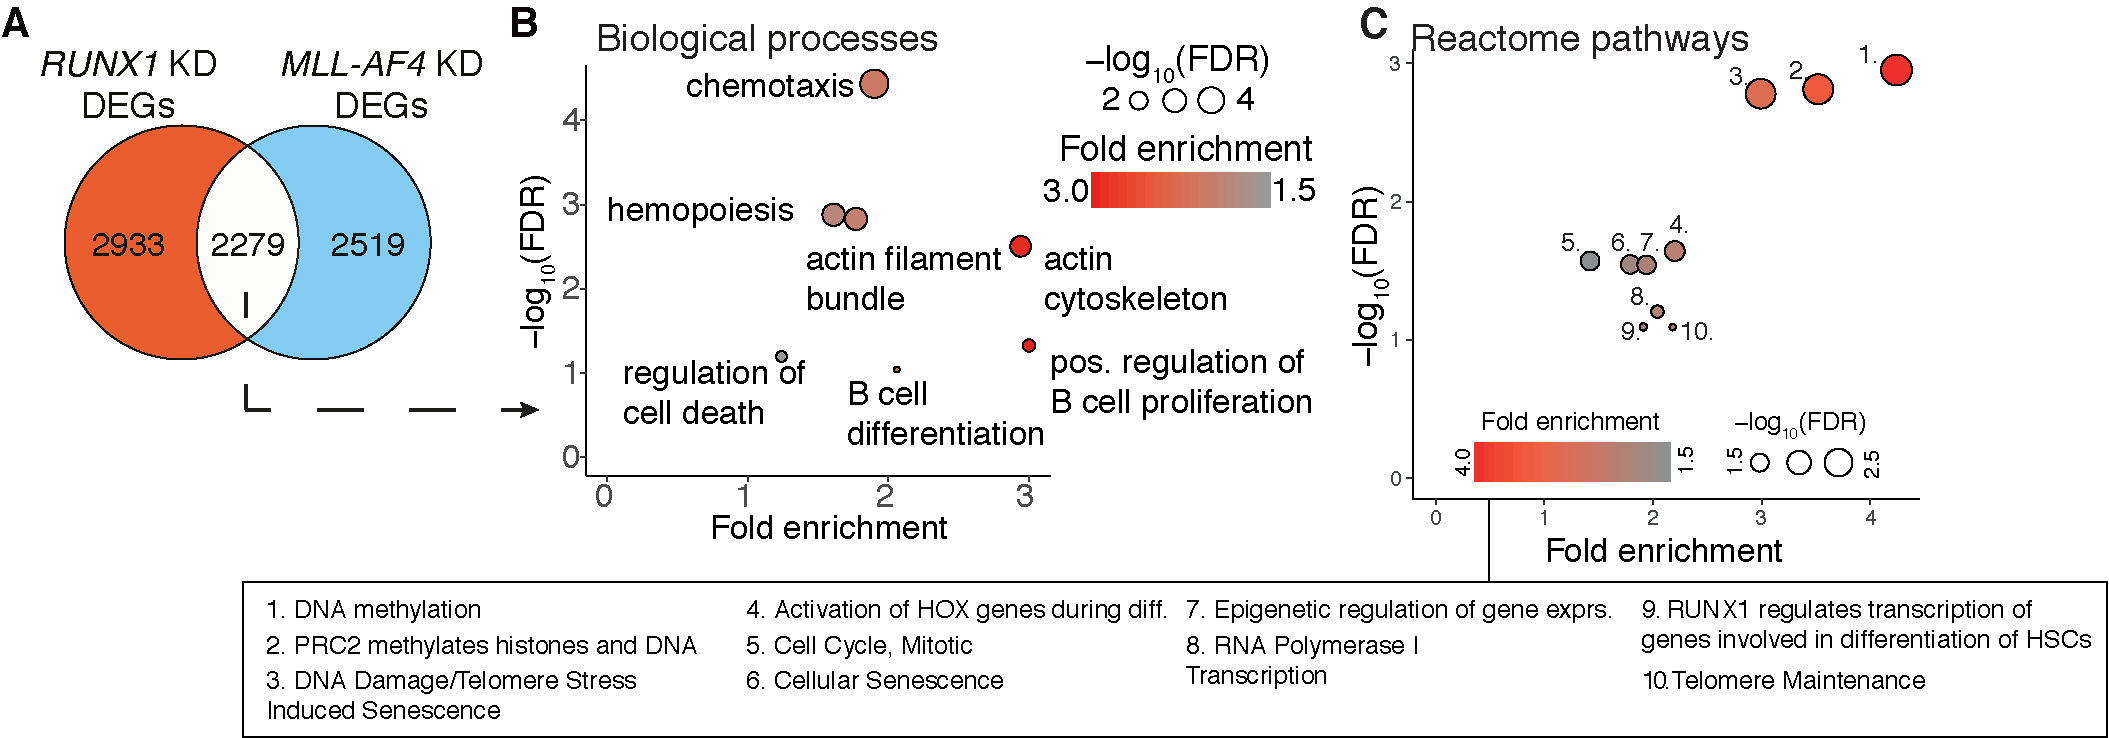
\includegraphics[width=\textwidth,height=\textheight,keepaspectratio]{figures/chapter4/chr4_interplay.png}
    %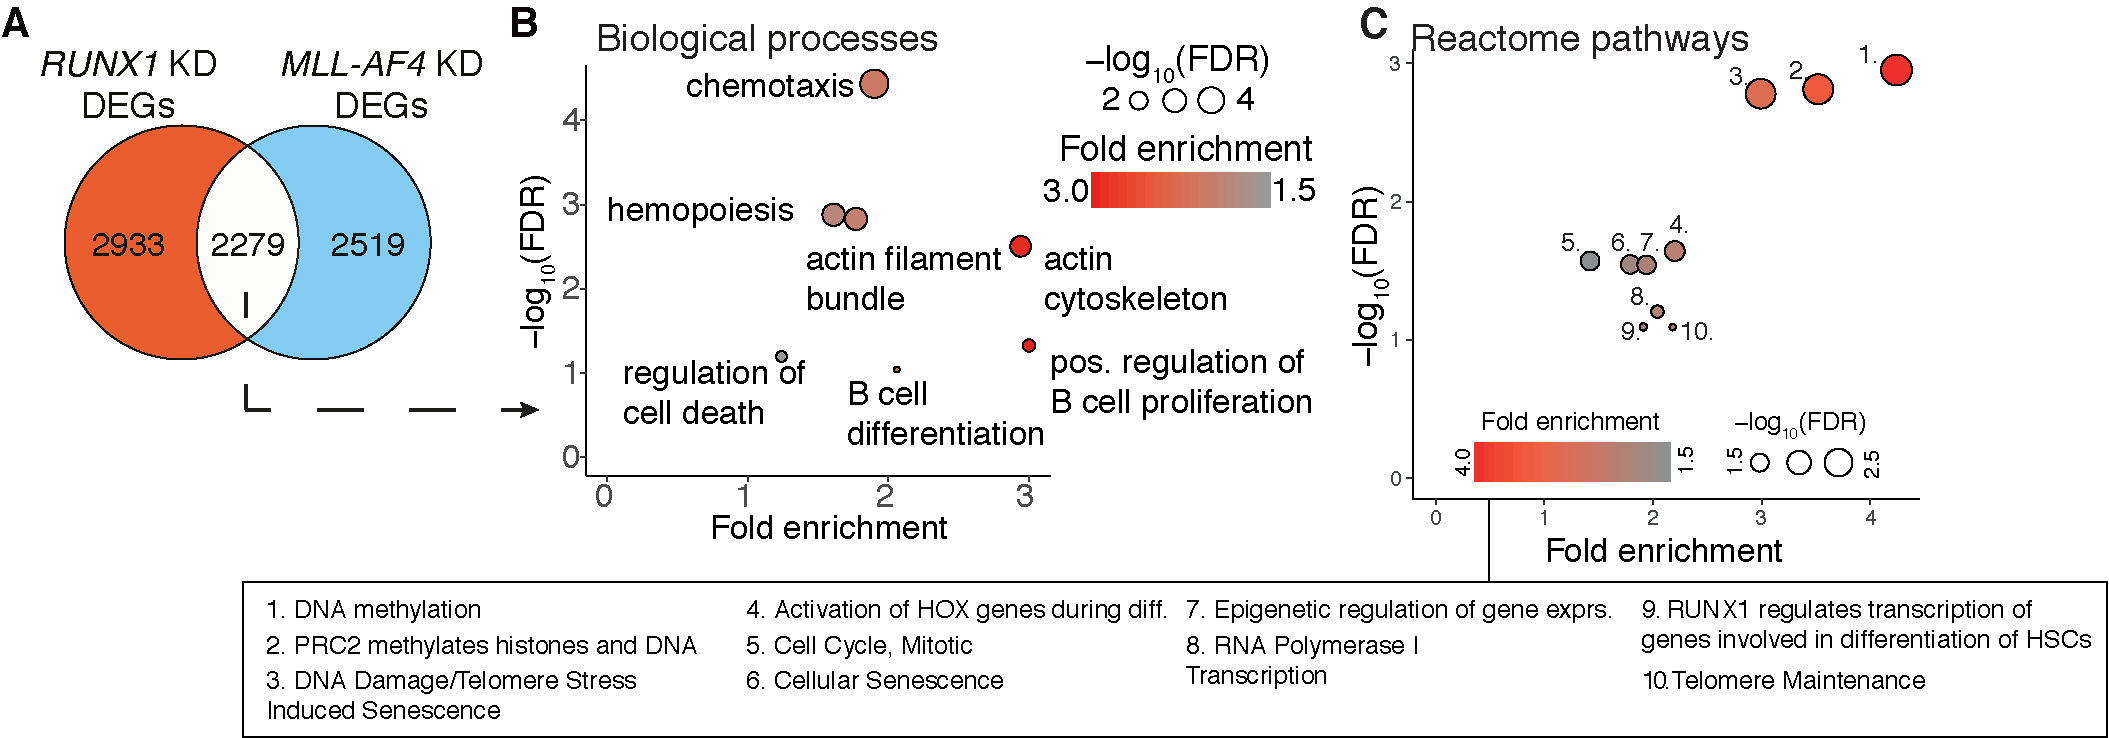
\includegraphics{figures/chapter4/chr4_interplay.png}
    \caption[{The overlap between MLL-AF4 and RUNX1 GRNs is enriched for processes promoting leukaemogenesis.}]
    {\textbf{The overlap between MLL-AF4 and RUNX1 GRNs is enriched for processes promoting leukaemogenesis.} 
    %\textbf{(A)} Distribution of logFC expression response to \textit{MLL-AF4} KD, \textit{RUNX1} KD, or EPZ-5675 treatment. LogFC response stratified by GRN-predicted direct or indirect regulation by MLL-AF4. 
    %\textbf{(B)} Reference-normalized ChIP-seq tracks for MLL-N and RUNX1 after 48 hours’ \textit{RUNX1} KD. 
    \textbf{(A)} Overlap between \textit{MLL-AF4} KD DEGs (Fig. \ref{fig:ch4_GRN_just}A) and RUNX1 KD DEGs (Fig. \ref{fig:ch4_runx1-grn}A-B). 
    \textbf{(B-C)} GO biological process (B) and reactome pathway (C) enrichment for overlap shown in A. 
    \textit{Adapted from \cite{harman_kmt2a-aff1_2021}.}
    }
    \label{fig:ch4_interplay}
\end{figure}

The central hypothesis of this chapter is that MLL-AF4 regulates a wider network through driving RUNX1 expression (Fig. \ref{fig:ch4_GRN_just}B), and the analysis so far has identified the TF RUNX1 as a key downstream effector of MLL-AF4 activity. Genes that are sensitive to both \textit{MLL-AF4} and \textit{RUNX1} KD in the GRN models (2279 DEGs, Fig. \ref{fig:ch4_interplay}A) were enriched for processes related to haematopoiesis, regulation of cell death, and B cell proliferation, consistent with an ALL expression program (Fig. \ref{fig:ch4_interplay}C). Pathway enrichment of these co-regulated genes revealed terms for epigenetic regulation such as DNA and histone methylation, cell cycle, and RUNX1 regulation (Fig. \ref{fig:ch4_interplay}C). These analyses suggest that the intersection of MLL-AF4 and RUNX1 GRNs drive a pro-leukaemic program.

\section{\label{ch4:ma4-runx1}MLL-AF4 and RUNX1 direct both FFL and TF cascade regulation}

\subsection{Identifying FFL and cascade regulatory circuits}

\begin{figure}[!t]
    \centering
    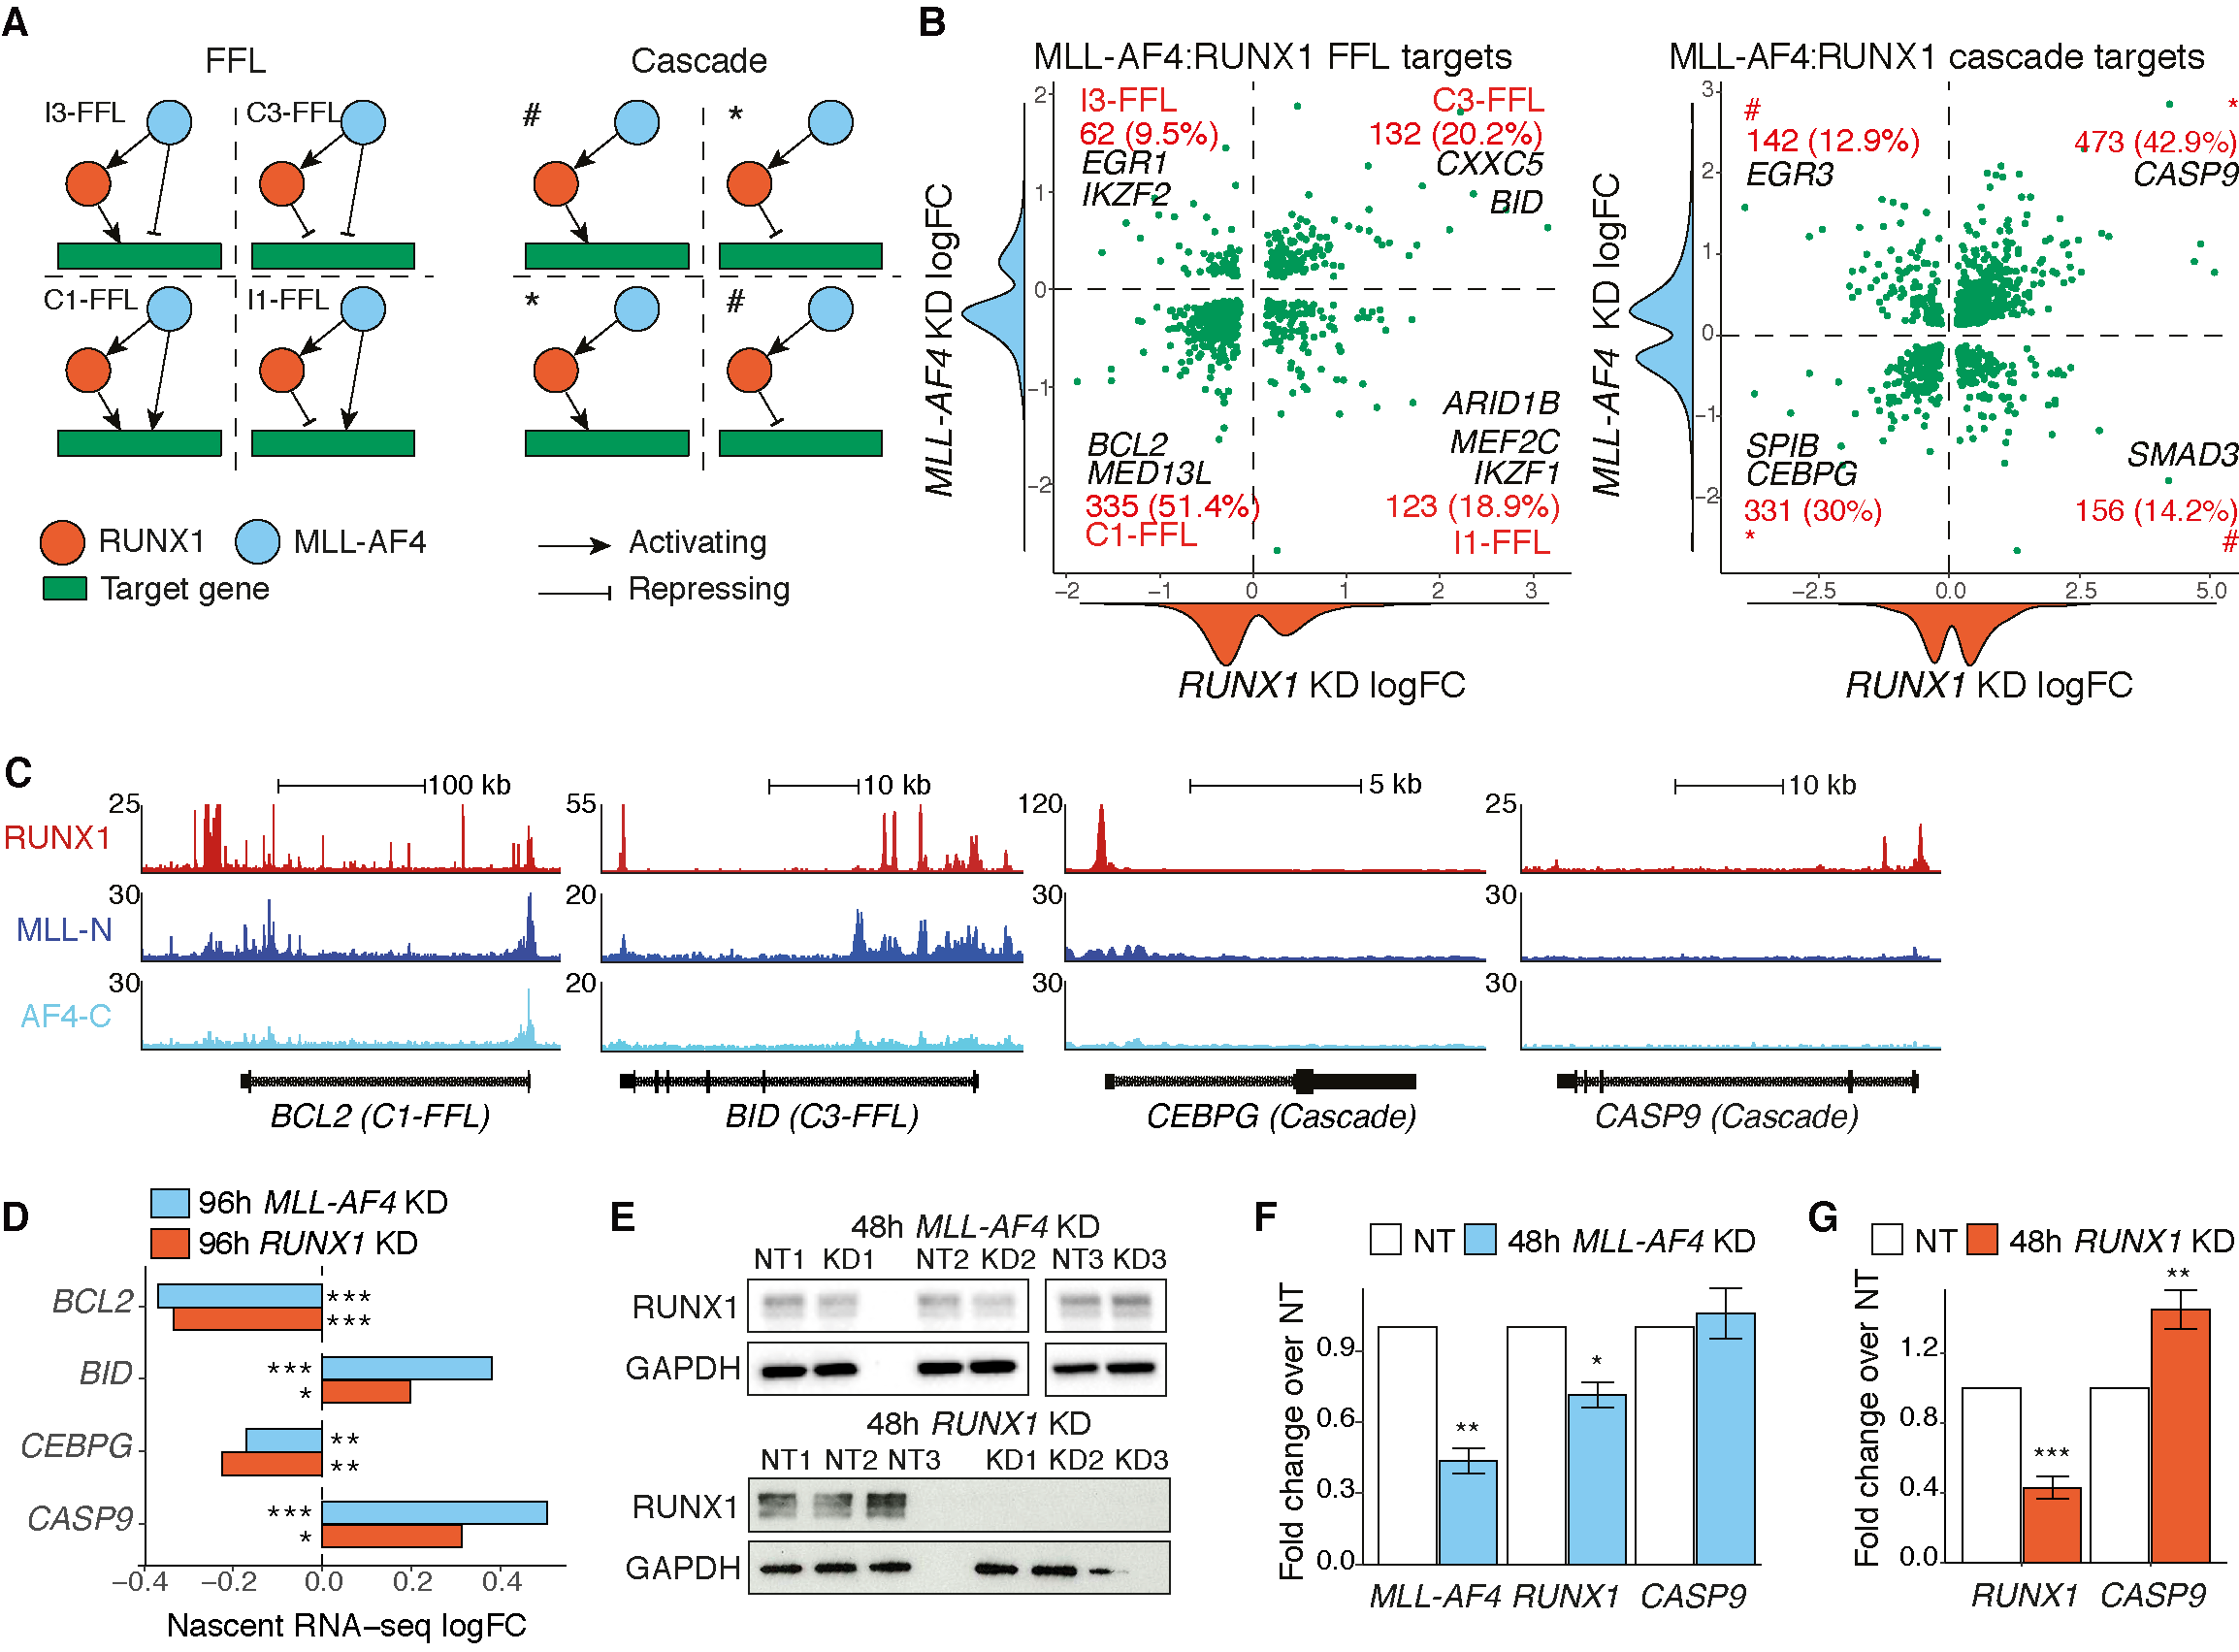
\includegraphics[width=\textwidth,height=\textheight,keepaspectratio]{figures/chapter4/chr4_grn-motifs.png}
    %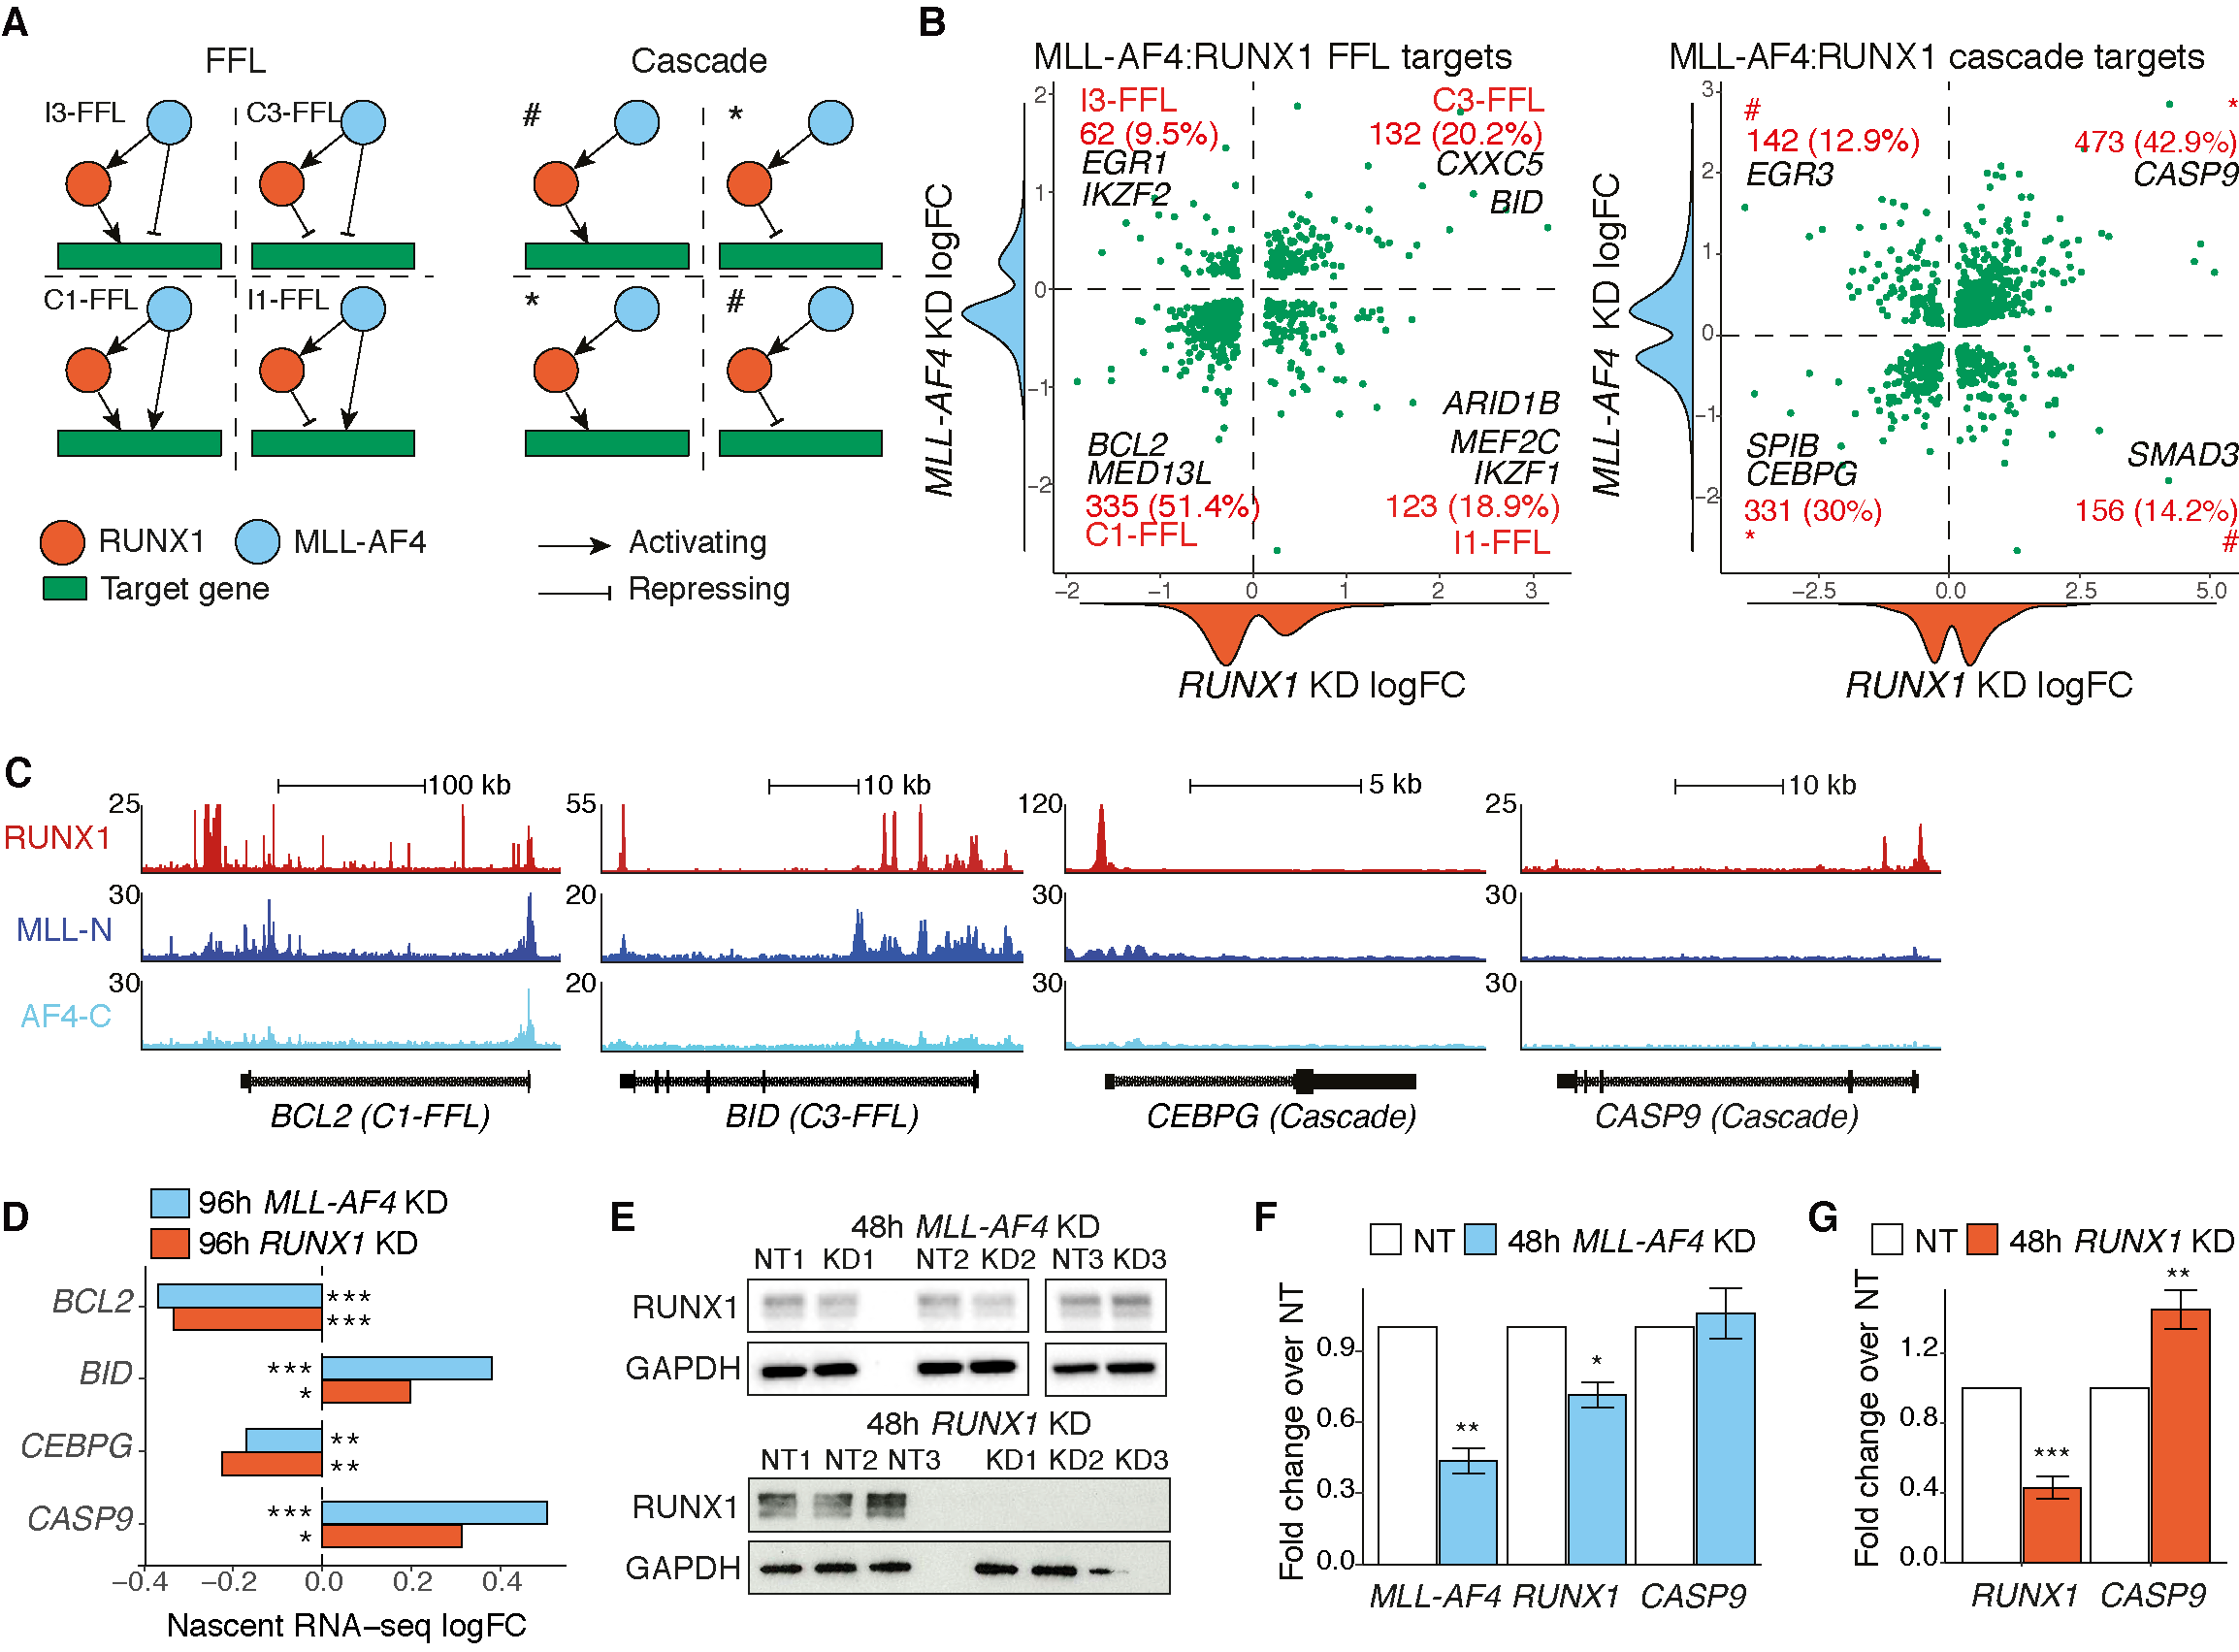
\includegraphics{figures/chapter4/chr4_grn-motifs.png}
    \caption[{Network motifs describing interplay between RUNX1 and MLL-AF4.}]
    {\textbf{Network motifs describing interplay between RUNX1 and MLL-AF4.} 
    \textbf{(A)} Illustration of FFL sub-types (left) and cascade (right) motifs. *: Same sign of effect. \#: Opposing sign of effect.
    \textbf{(B)} LogFC response to \textit{RUNX1} and \textit{MLL-AF4} KD in FFL (left) and TF cascade (right) target genes. Density plots of logFC distribution along axis. Quadrants of scatter plots align with FFL and cascade subtypes shown in A.
    \textbf{(C)} ChIP-seq tracks for MLL-N, AF4-C, and RUNX1 at \textit{BCL2} (C1-FFL target), \textit{BID} (C3-FFL target), \textit{CEBPG} and \textit{CASP9} (cascade targets). 
    \textbf{(D)} Nascent RNA-seq logFC following 96h \textit{RUNX1} or \textit{MLL-AF4} KD.
    \textbf{(E)} Western blot for RUNX1 protein in SEM cells after 48 h \textit{MLL-AF4} KD or 48 h \textit{RUNX1} KD, with GAPDH as loading control. 
    \textbf{(F, G)} qRT-PCR assaying \textit{MLL-AF4}, \textit{RUNX1} and \textit{CASP9} expression following 48 h \textit{MLL-AF4} KD (F) or 48 h \textit{RUNX1} KD (G) in SEM cells (\textit{n} = 3). 
    (*) P < 0.05; (**) P < 0.01; (***) P < 0.001
    \textit{Adapted from \cite{harman_kmt2a-aff1_2021}.}
    }
    \label{fig:ch4_motifs}
\end{figure}

While MLL-AF4 and RUNX1 regulatory logic intersects at key pathways, it is yet unclear whether these factors cooperate directly, or if this intersection is driven through RUNX1 acting as an intermediate TF. To dissect how RUNX1 and MLL-AF4 co-regulate gene targets I integrated the GRN models, then identified FFL and TF cascade regulatory motifs. Regulatory logic was predicted using the siRNA perturbation data (Fig. \ref{fig:ch4_GRN_just}A, Fig. \ref{fig:ch4_runx1-grn}A-B), where loss of gene expression upon KD implies positive regulation, and vice versa. This method assumes expression responses are a direct result of MLL-AF4 or RUNX1 regulation. It is well established that MLL-AF4 drives \textit{RUNX1} overexpression \citep{wilkinson_runx1_2013}, so this constrains possible FFL subtypes into just four categories. These include two coherent (C1- and C3-FFL) and two incoherent FFLs (I1- and I3-FFL), with subtypes classified by MLL-AF4 and RUNX1 regulation of genes \citep{mangan_structure_2003} (Fig. \ref{fig:ch4_motifs}A). Cascade motifs were identified as genes directly regulated by RUNX1, but indirectly (i.e., not bound) by MLL-AF4. These were further classified into so-called "coherent" and "incoherent" groups (Fig. \ref{fig:ch4_motifs}A, coherent and incoherent denoted by * and \# respectively). Coherent cascades show an alignment between the effect of \textit{RUNX1} and \textit{MLL-AF4} KD, which agrees with the hypothesis that RUNX1 targets a wider network as an intermediate for MLL-AF4.

Overall, we found that 71.6\% of FFLs were coherent, suggesting that MLL-AF4 and RUNX1 act cooperatively at the same loci (Fig. \ref{fig:ch4_motifs}B). For example, the key MLL-AF4 target \textit{BCL2} is activated in a C1-FFL, while \textit{BID} is repressed in a C3-FFL, with both loci bound by MLL-AF4 and RUNX1 (Fig. \ref{fig:ch4_motifs}C-D). FFL subtypes are typically biased towards a C1-FFL configuration \citep{joanito_incoherent_2018, mangan_incoherent_2006}, which is recapitulated in our analysis, with 51.5\% of FFLs showing cooperative activation of target genes (Fig. \ref{fig:ch4_motifs}B), further suggesting that RUNX1 at these FFL sites is biased towards activation. Interestingly, the EHT Runx1 target \textit{Ikzf1} (Fig. \ref{fig:ch3_pairwise}, p.\pageref{fig:ch3_pairwise}) is targeted in an I1-FFL in the MLL-AF4 GRN, where RUNX1 appears to repress \textit{IKZF1} rather than activate (RUNX1 KD logFC: 0.93, FDR: 2.8 x 10\textsuperscript{-43}), despite similar RUNX1 binding profiles to EHT (Fig. \ref{fig:ch4_runx1-grn}D). This change in RUNX1 regulation could be due to the leukaemic or the B cell context, in the presence of different cofactors and TFs.

The majority of cascade motifs are "coherent" (72.9\%, Fig. \ref{fig:ch4_motifs}B), suggesting that RUNX1 is a strong determining factor for regulation at the majority of cascade motifs. Example cascade targets are \textit{CEBPG} (activated) and \textit{CASP9} (repressed), where RUNX1 is bound but MLL-AF4 is not (Fig. \ref{fig:ch4_motifs}C-D). Incoherent cascades (27.1\%, Fig. \ref{fig:ch4_motifs}B) are likely a result of noise in the nascent RNA-seq experiments or regulatory control by additional TFs. Interestingly, while FFLs show a strong activation bias, cascade motifs are balanced between activating and repressive. This suggests that while RUNX1 behaves as an activator when at the same genes as MLL-AF4, at other sites RUNX1 may act as either an activator or a repressor. This is consistent with dual RUNX1 activity in haematopoietic differentiation \citep{kuvardina_runx1_2015, lutterbach_role_2000, canon_vivo_2003}.

The repressed cascade target \textit{CASP9} (caspase-9) was validated by performing siRNA KD for a shorter length of time. To generate the GRN, \textit{MLL-AF4} and \textit{RUNX1} KDs were performed for 96 hours to achieve a robust reduction in protein, resulting in significant \textit{CASP9} upregulation (Fig. \ref{fig:ch4_motifs}D); however, this timepoint also favours secondary effects. A shorter-term \textit{MLL-AF4} KD for 48 hours reduces \textit{RUNX1} mRNA levels, but does not impact RUNX1 protein, and has little effect on \textit{CASP9} expression (P = 0.64, Fig. \ref{fig:ch4_motifs}E-F), consistent with indirect regulation of \textit{CASP9} by MLL-AF4. \textit{CASP9} is upregulated with just 48 hours' \textit{RUNX1} KD, as with 96 hours' KD, suggesting that RUNX1 may directly repress the gene (Fig. \ref{fig:ch4_motifs}E, G). As \textit{CASP9} is sensitive to \textit{RUNX1} perturbation at an earlier timepoint, but not with \textit{MLL-AF4}, this confirms that MLL-AF4 may act in this TF cascade through RUNX1 activity.

\begin{figure}[t]
    \centering
    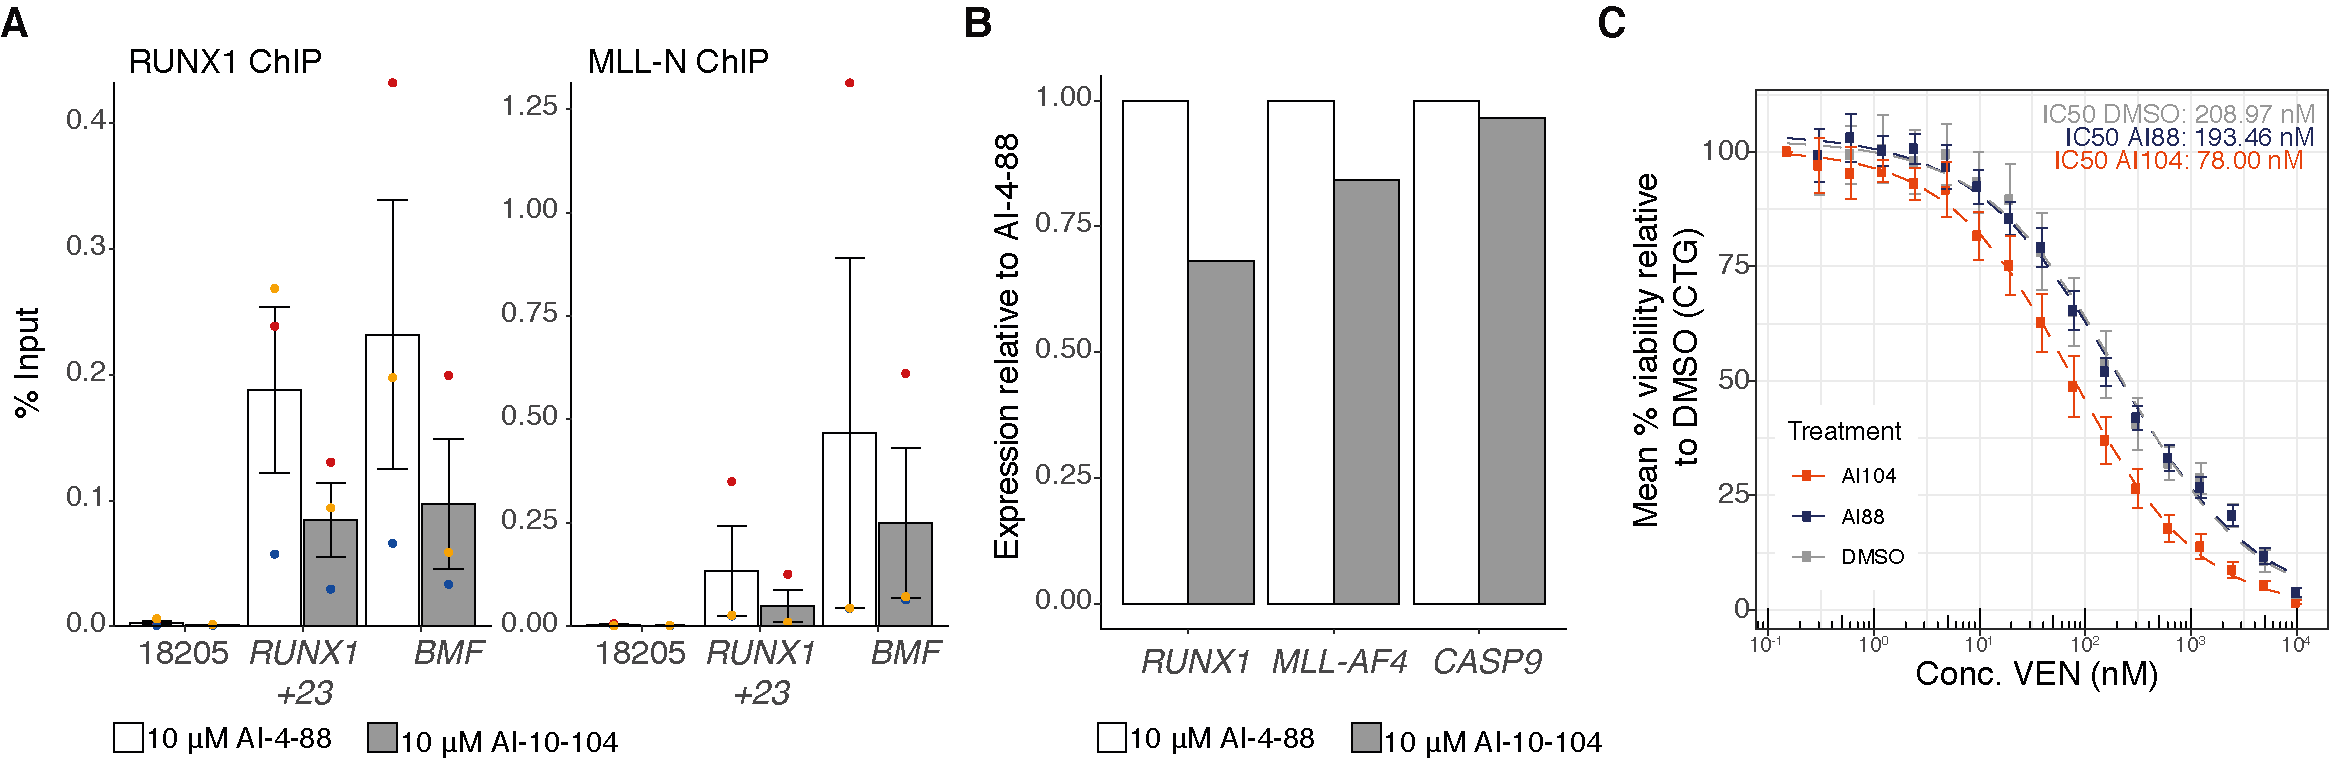
\includegraphics[width=\textwidth,height=\textheight,keepaspectratio]{figures/chapter4/chr4_runx1-inh.png}
    %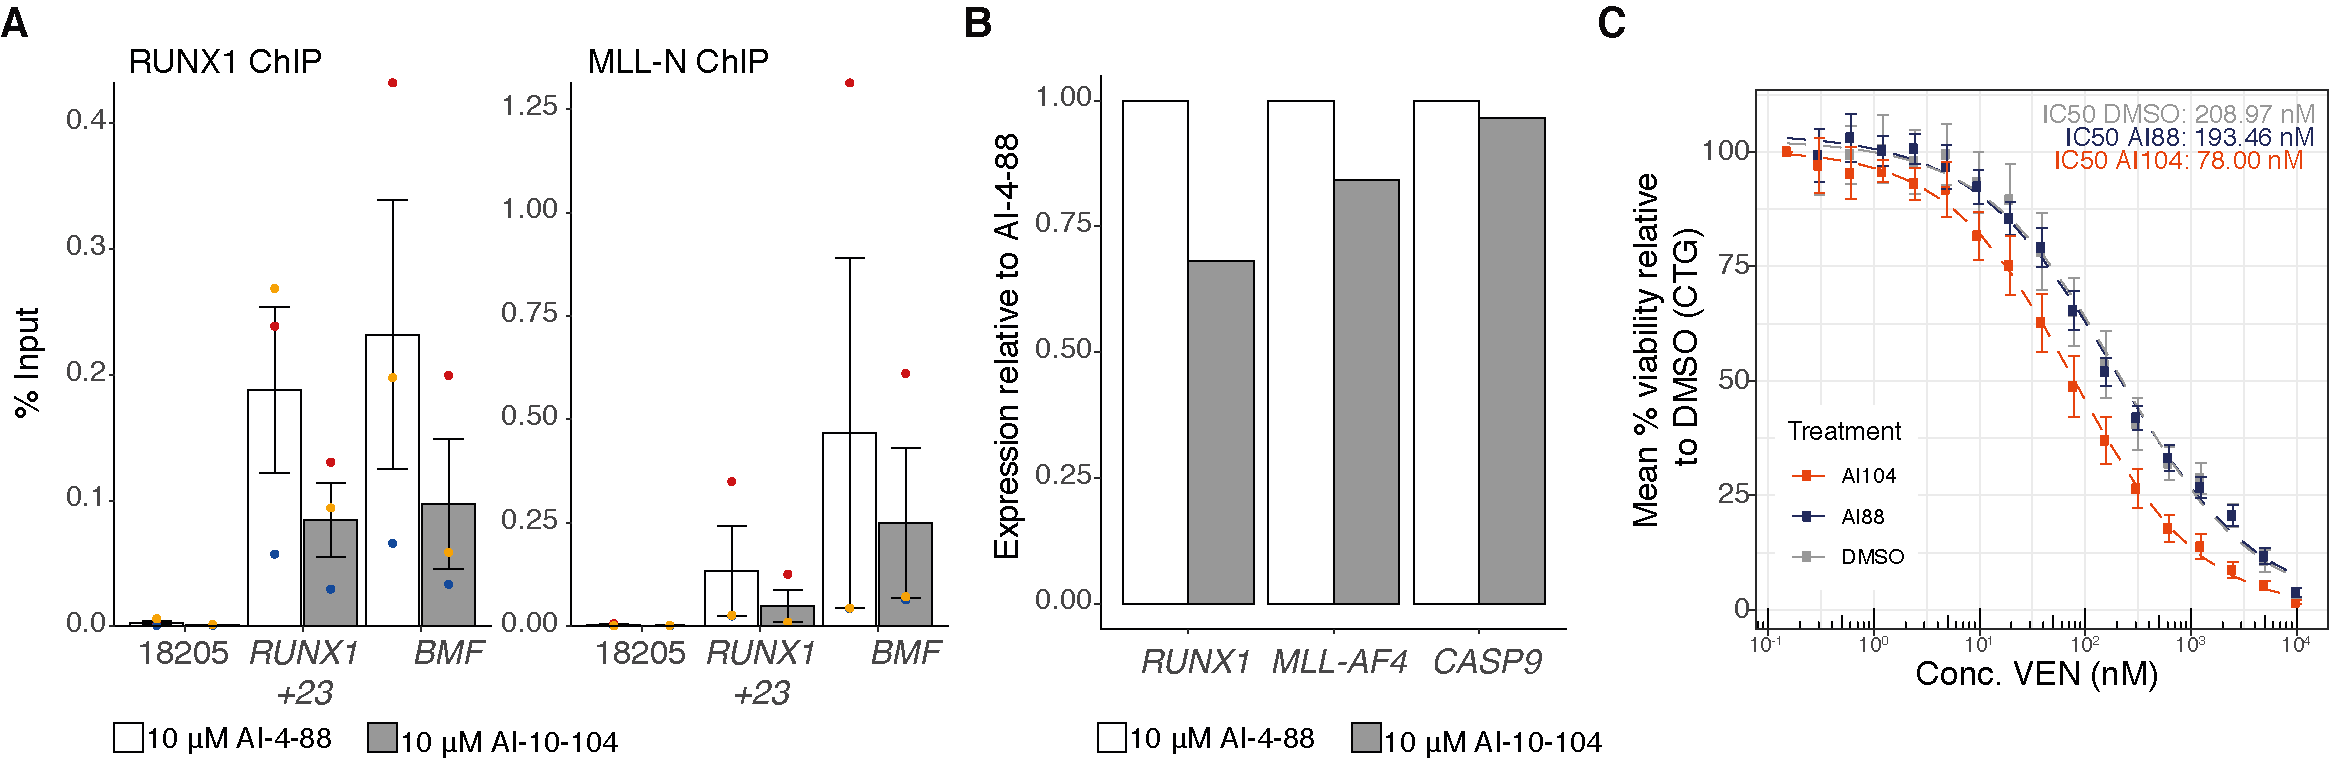
\includegraphics{figures/chapter4/chr4_runx1-inh.png}
    \caption[{RUNX1 inhibitor treatment reduces the IC50 concentration of venetoclax.}]
    {\textbf{RUNX1 inhibitor treatment reduces the IC50 concentration of venetoclax.} 
    \textbf{(A)} RUNX1 and MLL-N ChIP-qPCR after 24 h 10 \microm{} AI-10-104 or AI-4-88 (inactive control) treatment (as used in SEM cells in \cite{illendula_small_2016}), normalised to input chromatin. Regions probed are the \textit{RUNX1} +23 enhancer and a RUNX1 bound peak at the \textit{BMF} locus. 18205 refers to a negative control locus. Bars show mean, and error bars represent SEM (\textit{n} = 3).
    \textbf{(B)} qRT-PCR analysis showing \textit{RUNX1}, \textit{MLL-AF4}, and \textit{CASP9} expression after 24 h 10 \microm{} AI-10-104 or AI-4-88 (inactive control) treatment (\textit{n} = 1). Expression normalised to \textit{GAPDH} shown relative to AI-4-88.
    \textbf{(C)} Dose response curve of SEM cells treated with venetoclax for 24 h. Cells were co-treated with 10 \microm{} AI-10-104, AI-4-88 or DMSO). Viability measured using CTG, normalised to DMSO control. Dashed line represents dose response curve fit, and IC50 was calculated in the context of RUNX1 inhibitors. (\textit{n} = 8). 
    }
    \label{fig:ch4_runx1-inh}
\end{figure}

In publishing this data, in collaboration with M. Jamilly (Fulga lab), the MLL-AF4:RUNX1:\textit{CASP9} TF cascade was implicated as a potential promoter of venetoclax resistance \citep{harman_kmt2a-aff1_2021}. Venetoclax is a BCL2 inhibitor that is used to treat \textit{MLL}r leukaemia \citep{khaw_venetoclax_2016, vandenberg_abt-199_2013}, though drug resistance is a concern. As caspase-9 lies downstream of BCL2 in the apoptotic pathway, the MLL-AF4:RUNX1:\textit{CASP9} cascade may provide a potential circuit for deterring apoptosis. To test whether RUNX1 activity interacts with venetoclax efficacy, I treated SEM cells with a small molecule RUNX1 inhibitor (active AI-10-104, inactive AI-4-88) that disrupts RUNX1 binding to the TF CBF$\beta$ \citep{illendula_small-molecule_2015, illendula_small_2016}, resulting in reduced RUNX1 DNA binding and expression (Fig. \ref{fig:ch4_runx1-inh}A-B). This reduced \textit{RUNX1} expression is likely due to loss of positive RUNX1 autoregulation \citep{martinez_transcriptional_2016}. I generated venetoclax dose-response curves, and co-treated with 10 \microm{} RUNX1 inhibitor. Co-treatment with AI-10-104 yielded a lower venetoclax IC50 (78 nM) over AI-4-88 or DMSO treatment (208.97 nM, 193.47 nM) (Fig. \ref{fig:ch4_runx1-inh}C). This preliminary analysis suggests an interaction between venetoclax and RUNX1 activity, though \textit{CASP9} levels appear unaffected by RUNX1 inhibition, so it is possible that this effect is mediated through alternative pathways (Fig. \ref{fig:ch4_runx1-inh}B). Additional replicates are needed to determine \textit{CASP9} sensitivity to AI-10-104 treatment. Recent studies have noted improved venetoclax response in patients with \textit{RUNX1} mutations, and have suggested this effect is through generally reducing the apoptotic threshold \citep{cherry_venetoclax_2021, chow_runx1_2021}. A more robust experimental design is required to determine if the effect is synergistic.

\subsection[Correlation between MLL-AF4 and RUNX1 ChIP-seq binding profiles]{\label{ch4:ma4-runx1-cor}Correlation between MLL-AF4 and RUNX1\\ChIP-seq binding profiles}

The number of MLL-AF4:RUNX1 FFLs and the shared regulatory logic at these genes suggests a synergistic interaction between the two factors. To investigate this possibility, I performed correlative analyses of genome wide chromatin binding profiles. For the TFs analysed (RUNX1 and MAZ), there was reasonable correlation with MLL-N ChIP-seq signal at promoters (Fig. \ref{fig:ch4_ma4-TF-cor}A), and genome wide binding patterns show general co-localisation of the TFs and MLL-N (Fig. \ref{fig:ch4_ma4-TF-cor}B). MLL-AF4 binding is broader than TFs peaks, and MLL-FP spreading is associated with highly overexpressed targets \citep{kerry_mll-af4_2017} (Fig. \ref{fig:ch4_ma4-TF-cor}A), making precise comparisons between MLL-AF4 and TFs difficult. However, with increased MLL-AF4 spreading I observed a similar spread of TF binding, with an increased number of TF peaks. This is exemplified at \textit{GNAQ}, where rather than typical spreading, a higher frequency of TF binding can be seen co-localising with MLL-AF4 spreading (Fig. \ref{fig:ch4_ma4-TF-cor}A).

\begin{figure}[htbp]
    \centering
    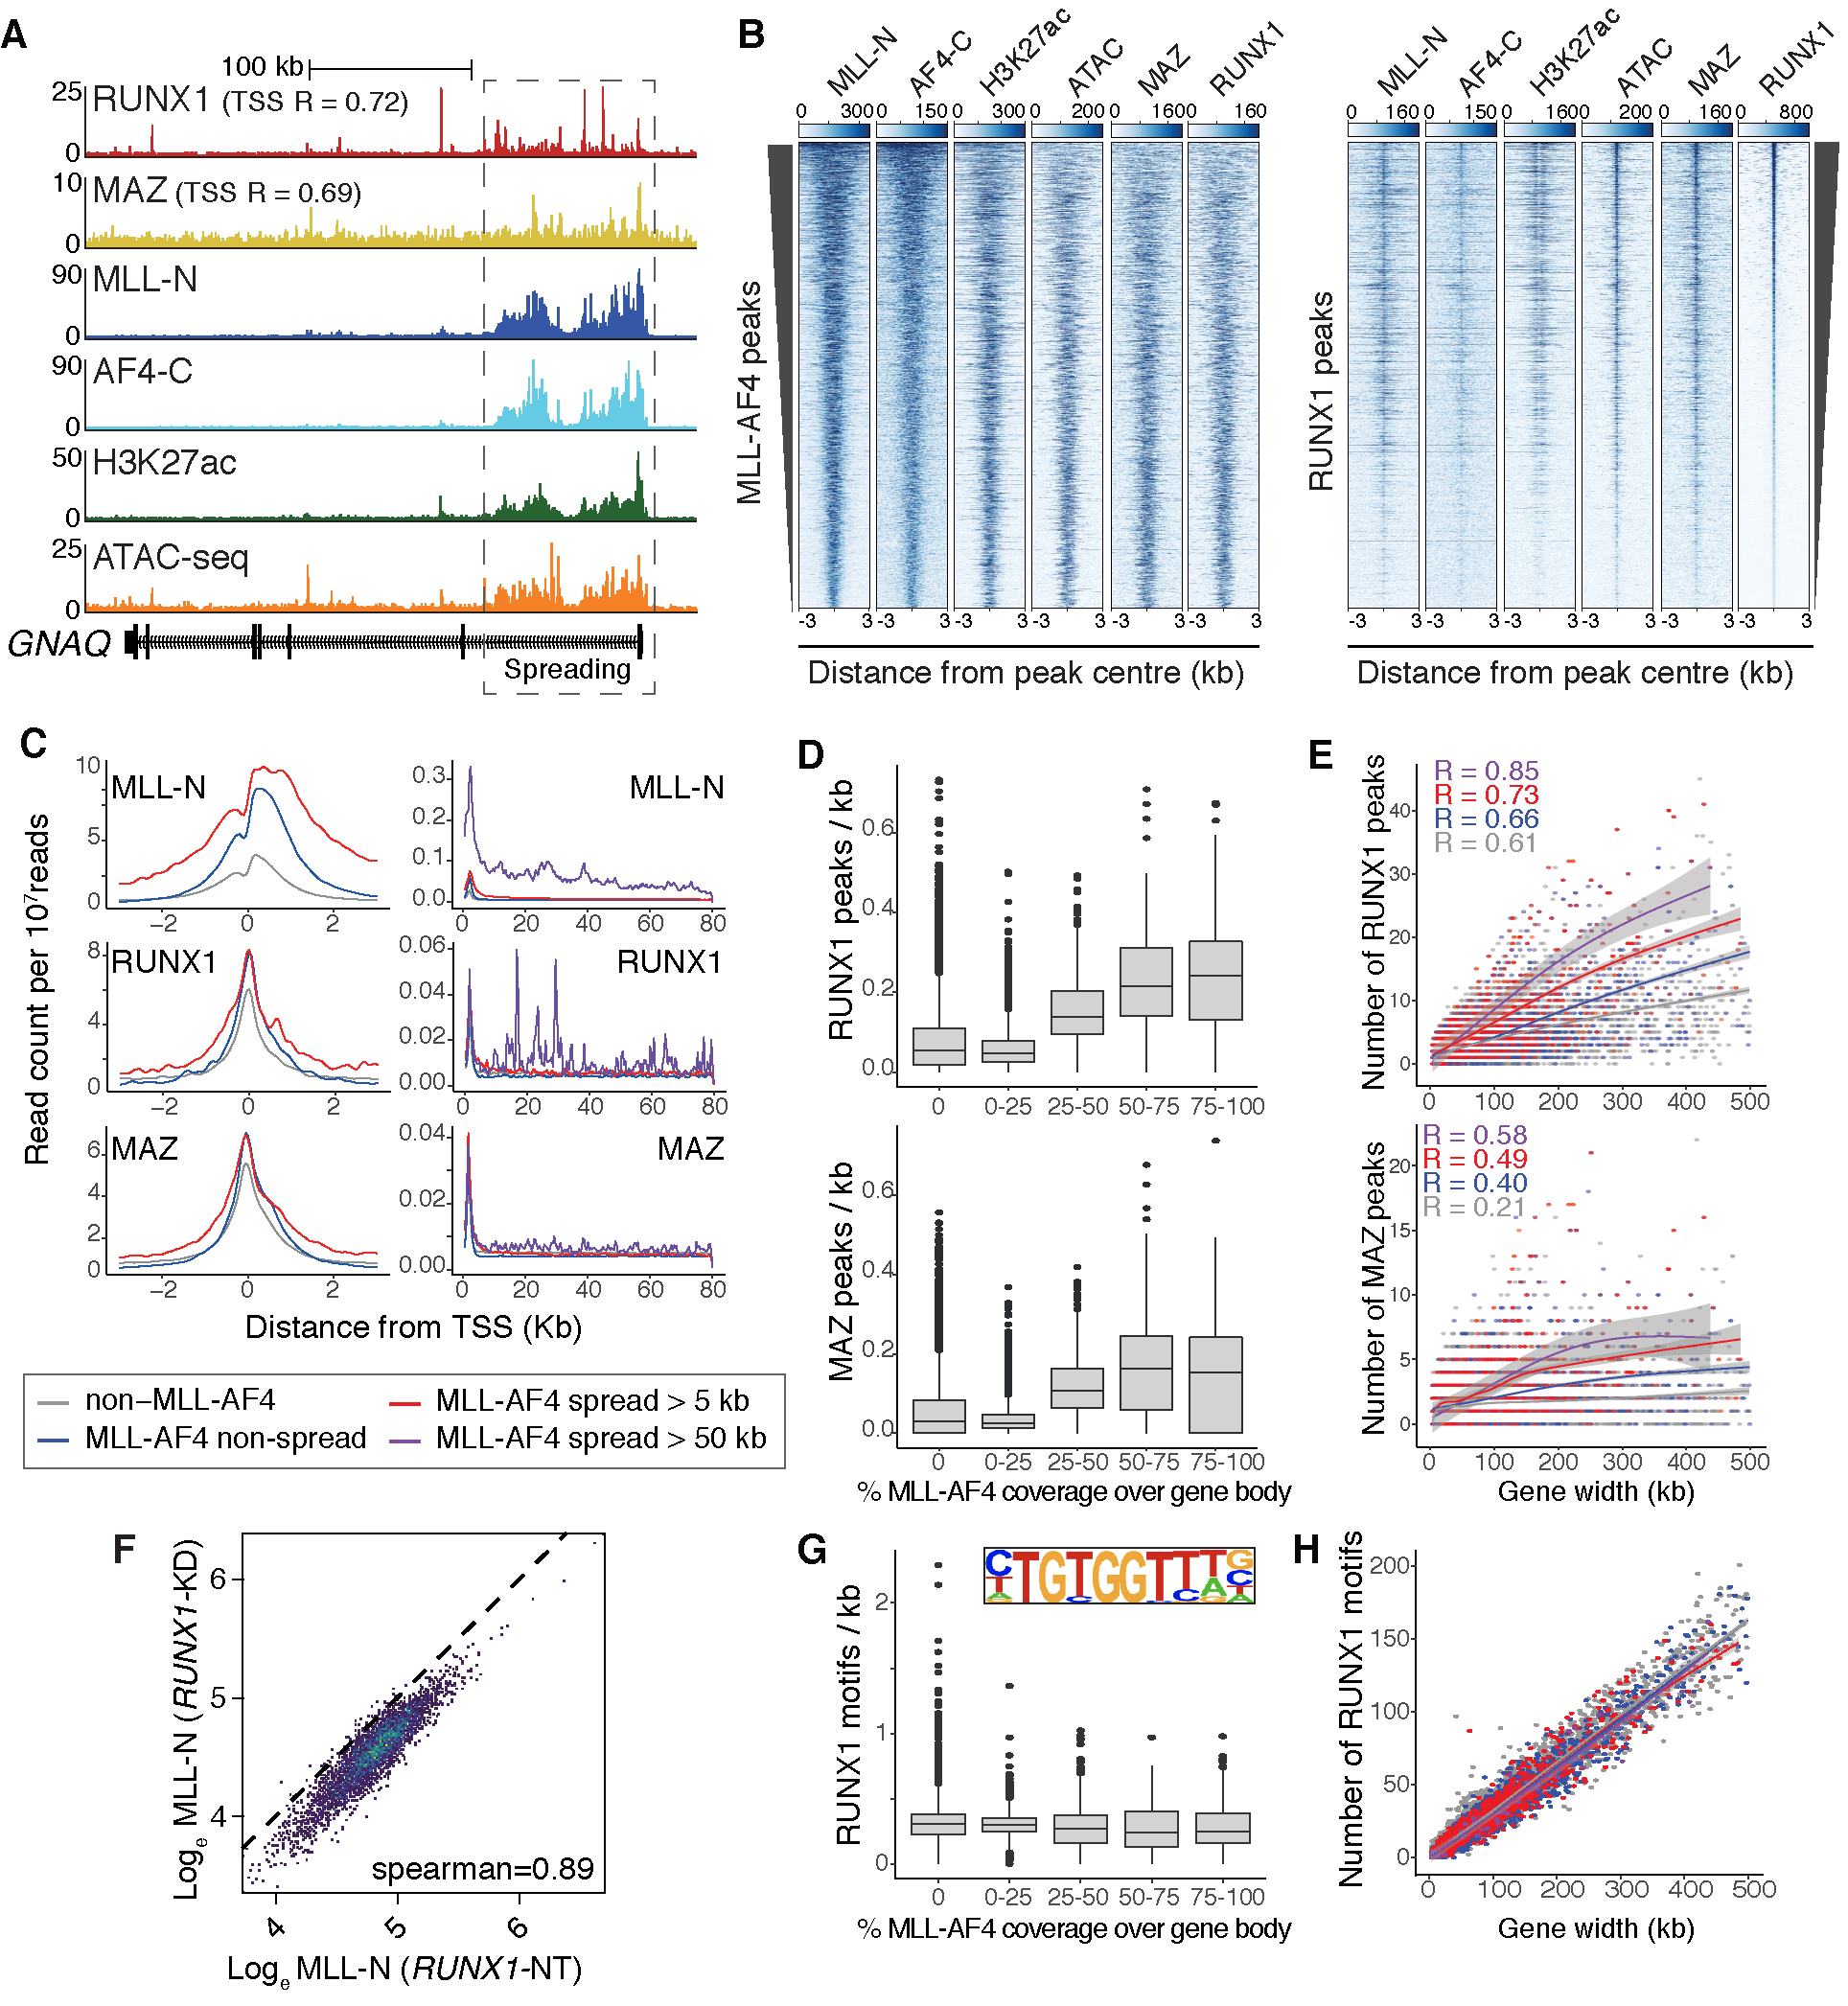
\includegraphics[width=\textwidth,height=\textheight,keepaspectratio]{figures/chapter4/chr4_ma4-TF-correlation.png}
    %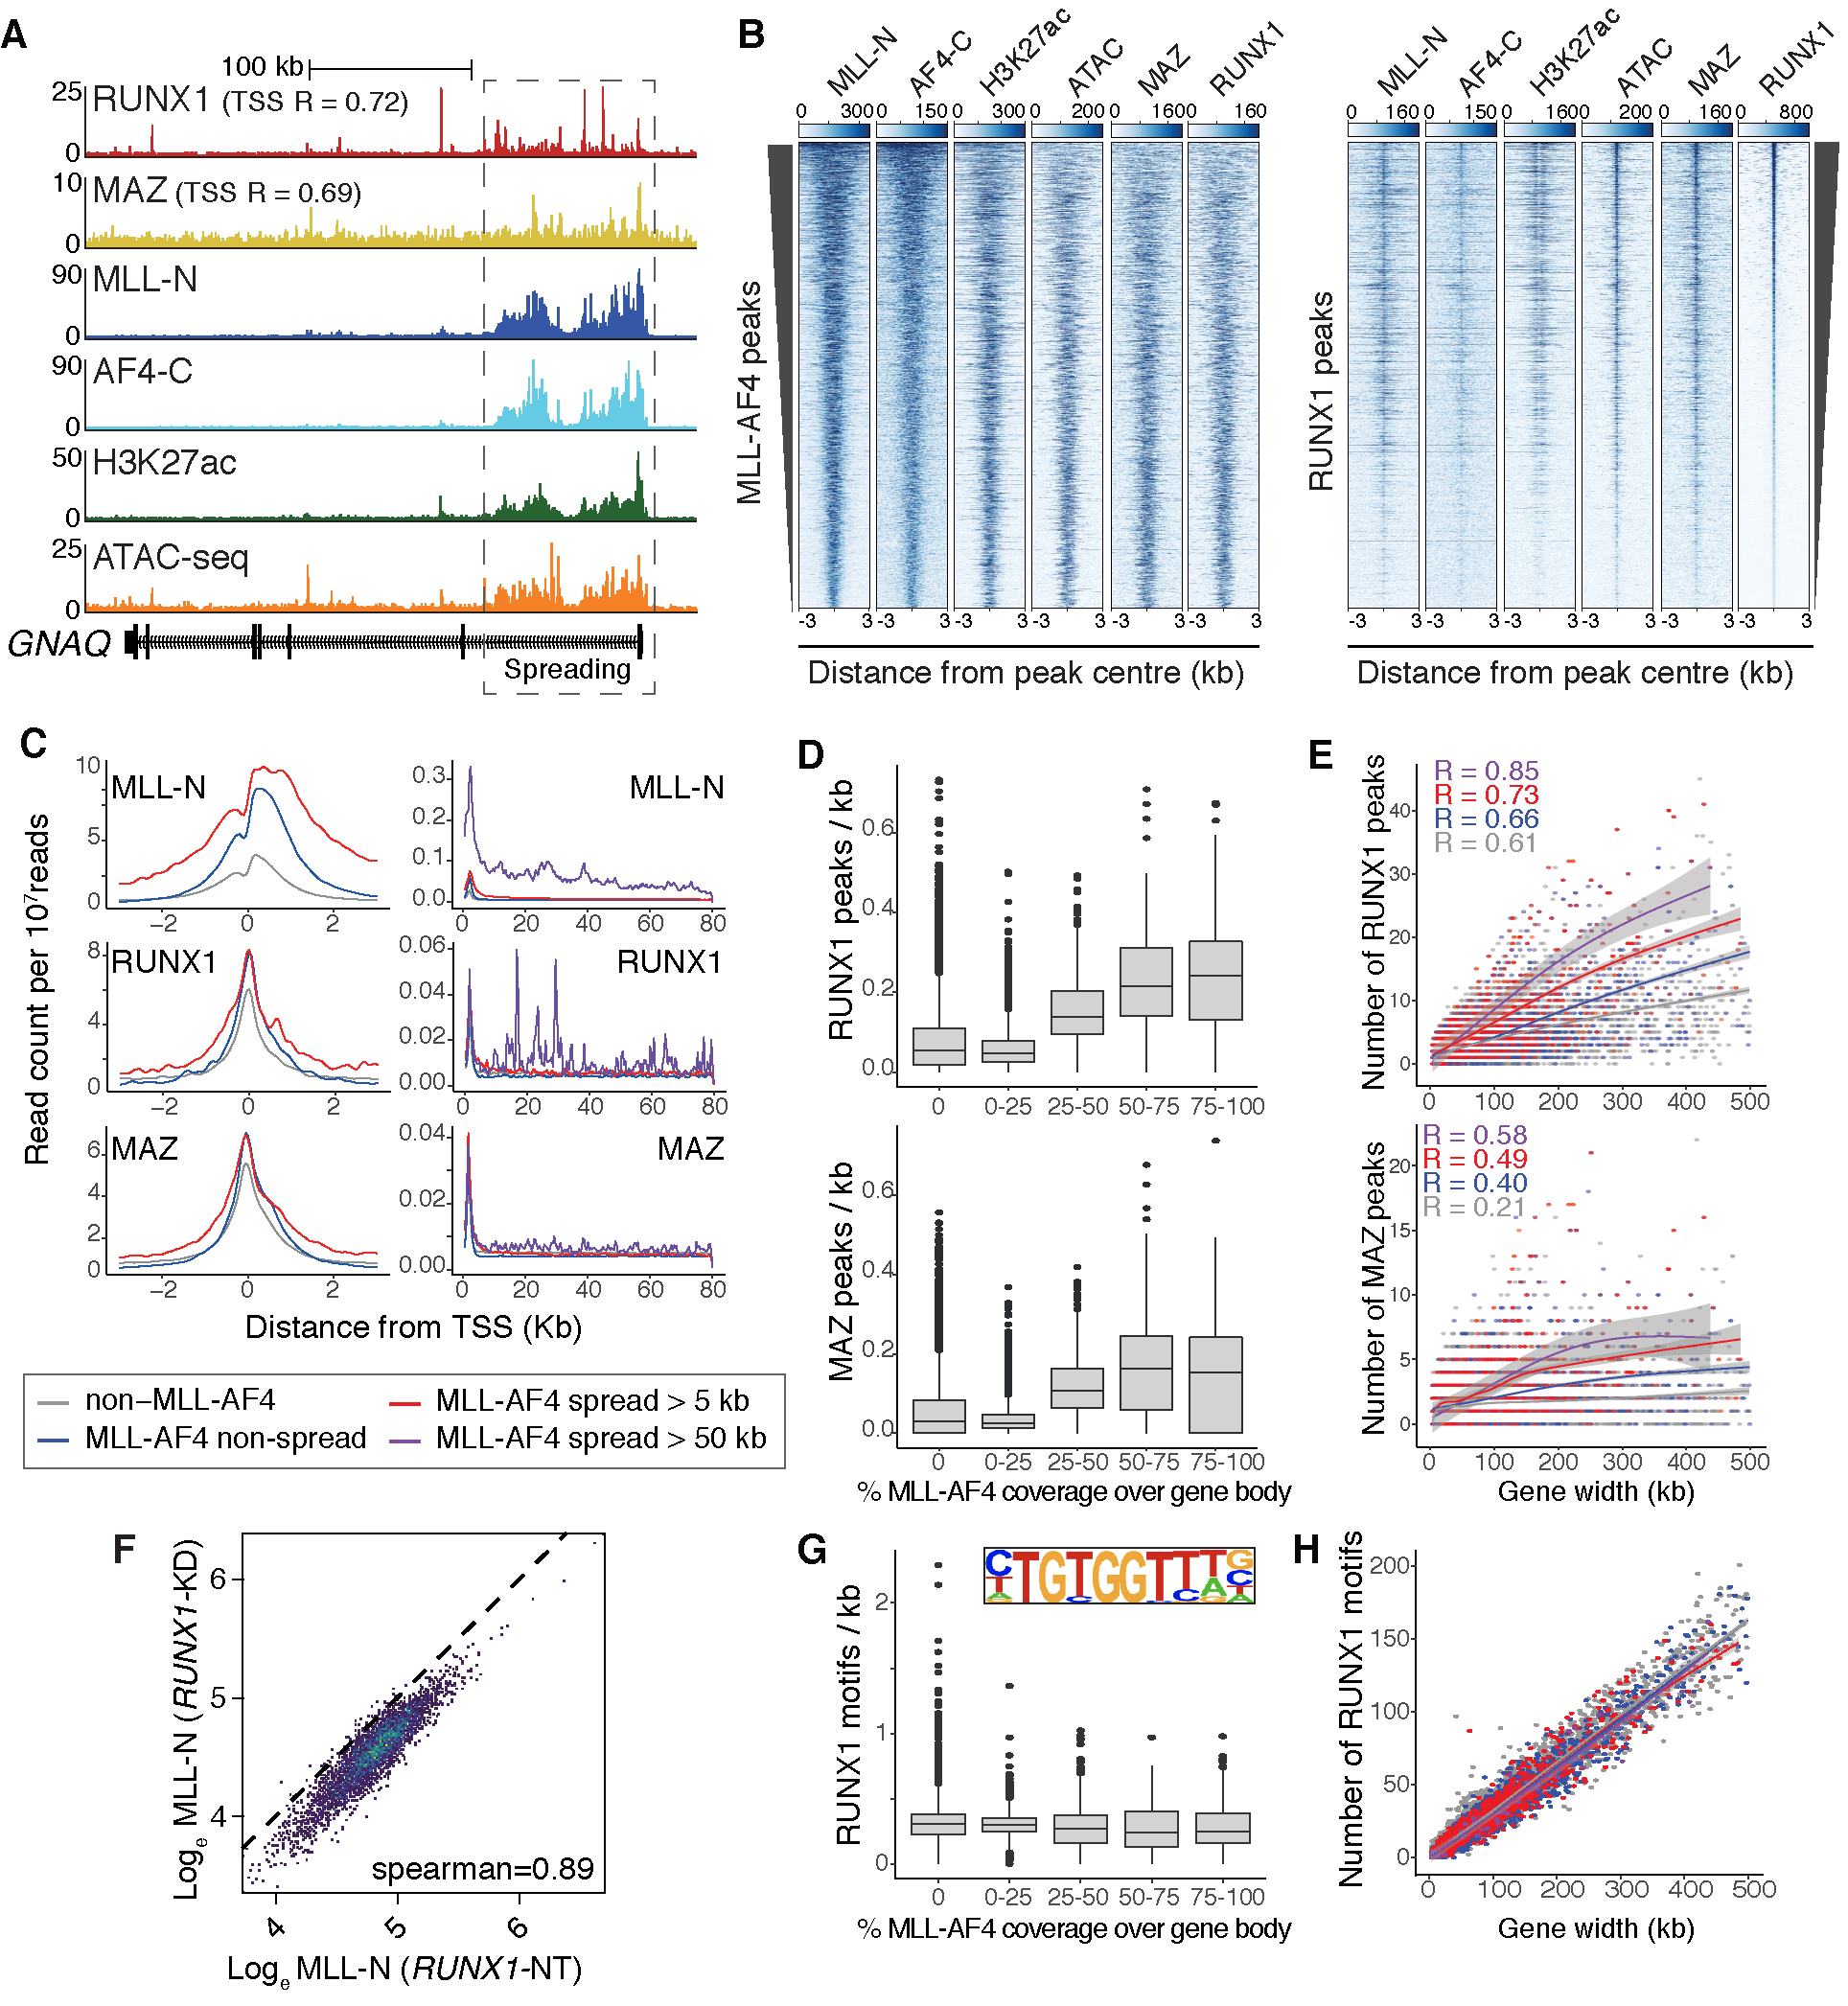
\includegraphics{figures/chapter4/chr4_ma4-TF-correlation.png}
    \caption[{MLL-AF4 establishes an environment encouraging TF binding and FFL formation.}]
    {\textbf{MLL-AF4 establishes an environment encouraging TF binding and FFL formation.} 
    \textbf{(A)} ChIP-seq tracks for GRN TFs, H3K27ac and ATAC-seq at \textit{GNAQ}. Correlation (\textit{R}) comparing TF ChIP-seq signal with MLL-N over expressed gene promoters. Dashed box highlights MLL-AF4 spreading.
    \textbf{(B)} ChIP-seq and ATAC-seq heatmaps in SEM cells, at MLL-AF4 peaks (left) and RUNX1 peaks (right), ordered by ChIP-seq signal.
    \textbf{(C)} Mean ChIP-seq signal at expressed promoters over a 6 kb (left) or 80 kb (right) window. Profiles stratified by MLL-AF4 binding classes as labelled.
    \textbf{(D,G)} TF ChIP-seq peaks/kb (D) or RUNX1 motifs/kb (G) over gene bodies, stratified by proportion of MLL-AF4 coverage.
    \textbf{(E,H)} Relationship between TF peak (E) or RUNX1 motif (H) frequency over gene bodies, and gene body length (kb), stratified by MLL-AF4 binding classes as in C. Local regression (LOESS) lines fit with 95\% CI in grey. Correlation (\textit{R}) calculated by MLL-AF4 binding classes. RUNX1 motif logo shown.
    \textbf{(F)} Log\textsubscript{e} MLL-N ChIP-seq reads at MLL-AF4 peaks following 48 hours’ treatment with NT or RUNX1 siRNA. 
    }
    \label{fig:ch4_ma4-TF-cor}
\end{figure}

To test whether increased TF binding is associated with MLL-AF4 genome wide, I analysed TF peak densities at gene loci. I first classified expressed genes by MLL-AF4 spreading status, differentiating between > 5 kb spreading (754 genes) and > 50 kb spreading (25 genes). TF binding at promoters was more intense at all MLL-AF4 targets over non-MLL-AF4, and showed increased signal outside the promoter at spreading targets. Further, with > 50 kb spreading there was increased TF signal over 50 kb away from gene promoters (Fig. \ref{fig:ch4_ma4-TF-cor}C). The density of TF ChIP-seq peaks across a gene body (peaks/kb) increased with a greater proportion of MLL-AF4 coverage (Fig. \ref{fig:ch4_ma4-TF-cor}D). The relationship between total TF peaks and gene body length is also stronger at MLL-AF4 spreading targets over non-spreading or unbound genes (Fig. \ref{fig:ch4_ma4-TF-cor}E). The TF peak density at spreading targets is much higher with RUNX1 than MAZ, though the relationship is present in both cases. Together this suggests that with a greater spread of MLL-AF4 there is an increased frequency of TF binding. 

As this analysis is correlative, whether TF binding encourages MLL-AF4 spreading or MLL-AF4 drives TF binding remains unclear. To determine whether TFs may influence MLL-AF4 binding or spreading patterns I first performed \textit{RUNX1} siRNA KD. With 48 hours' \textit{RUNX1} KD MLL-AF4 binding genome wide is slightly reduced, though profiles are largely maintained with no site-specific loss of MLL-AF4 and high correlation between KD and control samples (Fig. \ref{fig:ch4_ma4-TF-cor}F). The slight reduction in MLL-AF4 binding could reflect a subtle impact on MLL-AF4 protein levels, though nascent \textit{MLL-AF4} expression is unaffected (96h \textit{RUNX1} KD RNA-seq: logFC = 0.1, FDR = 0.12). It remains difficult to disentangle the effect of \textit{MLL-AF4} perturbation on RUNX1 binding, as MLL-AF4 directly drives \textit{RUNX1} expression. Therefore, I cannot confidently conclude that MLL-AF4 directs TF binding, though the correlation is suggestive. Importantly, while RUNX1 binding frequency increases with MLL-AF4 spreading, RUNX1 motifs do not (Fig. \ref{fig:ch4_ma4-TF-cor}G-H). This could imply the increased TF binding is through non-sequence specific DNA binding mechanisms, such as association with larger protein complexes, or that RUNX1 motifs are in equal excess across genes and MLL-AF4 establishes increased RUNX1 motif binding affinity. This analysis suggests that MLL-AF4 and TFs co-localise to form FFL circuits, in a process that may be driven by MLL-AF4. An attractive hypothesis is that MLL-AF4 increases the binding affinity of TFs for existing motifs, through epigenetic modification and increased chromatin accessibility.

\section{\label{ch4:tf-cointeraction}TF cooperation at MLL-AF4 targets drives expression and promotes leukaemogenesis}

The data presented thus far offer a breakdown of MLL-AF4 and TF cooperation in FFLs, and indirect MLL-AF4 regulation using TFs as intermediates in cascade motifs. FFL motifs are particularly prominent, and there appears to be a relationship between MLL-AF4 and TF binding, promoting co-localisation at MLL-AF4 target sites. As MLL-AF4 and RUNX1 networks intersect at regulation of cell death and cell cycle processes (Fig. \ref{fig:ch4_interplay}B), it is likely that RUNX1 drives regulation of these processes. Key genes that regulate proliferation and apoptosis include \textit{MYC} \citep{dang_myc_2012} and \textit{BCL2} \citep{kale_bcl-2_2018}. MLL-AF4 regulates both of these factors \citep{robinson_abundant_2008, benito_mll-rearranged_2015}, and as MLL-AF4 appears to increase TF binding affinity (Fig. \ref{fig:ch4_motifs} and Fig. \ref{fig:ch4_ma4-TF-cor}), the overexpression of these genes may be partly driven by cooperative TF activity. I therefore investigated whether RUNX1 co-interacts with other TFs to drive \textit{BCL2} and \textit{MYC} expression.

\begin{figure}[t]
    \centering
    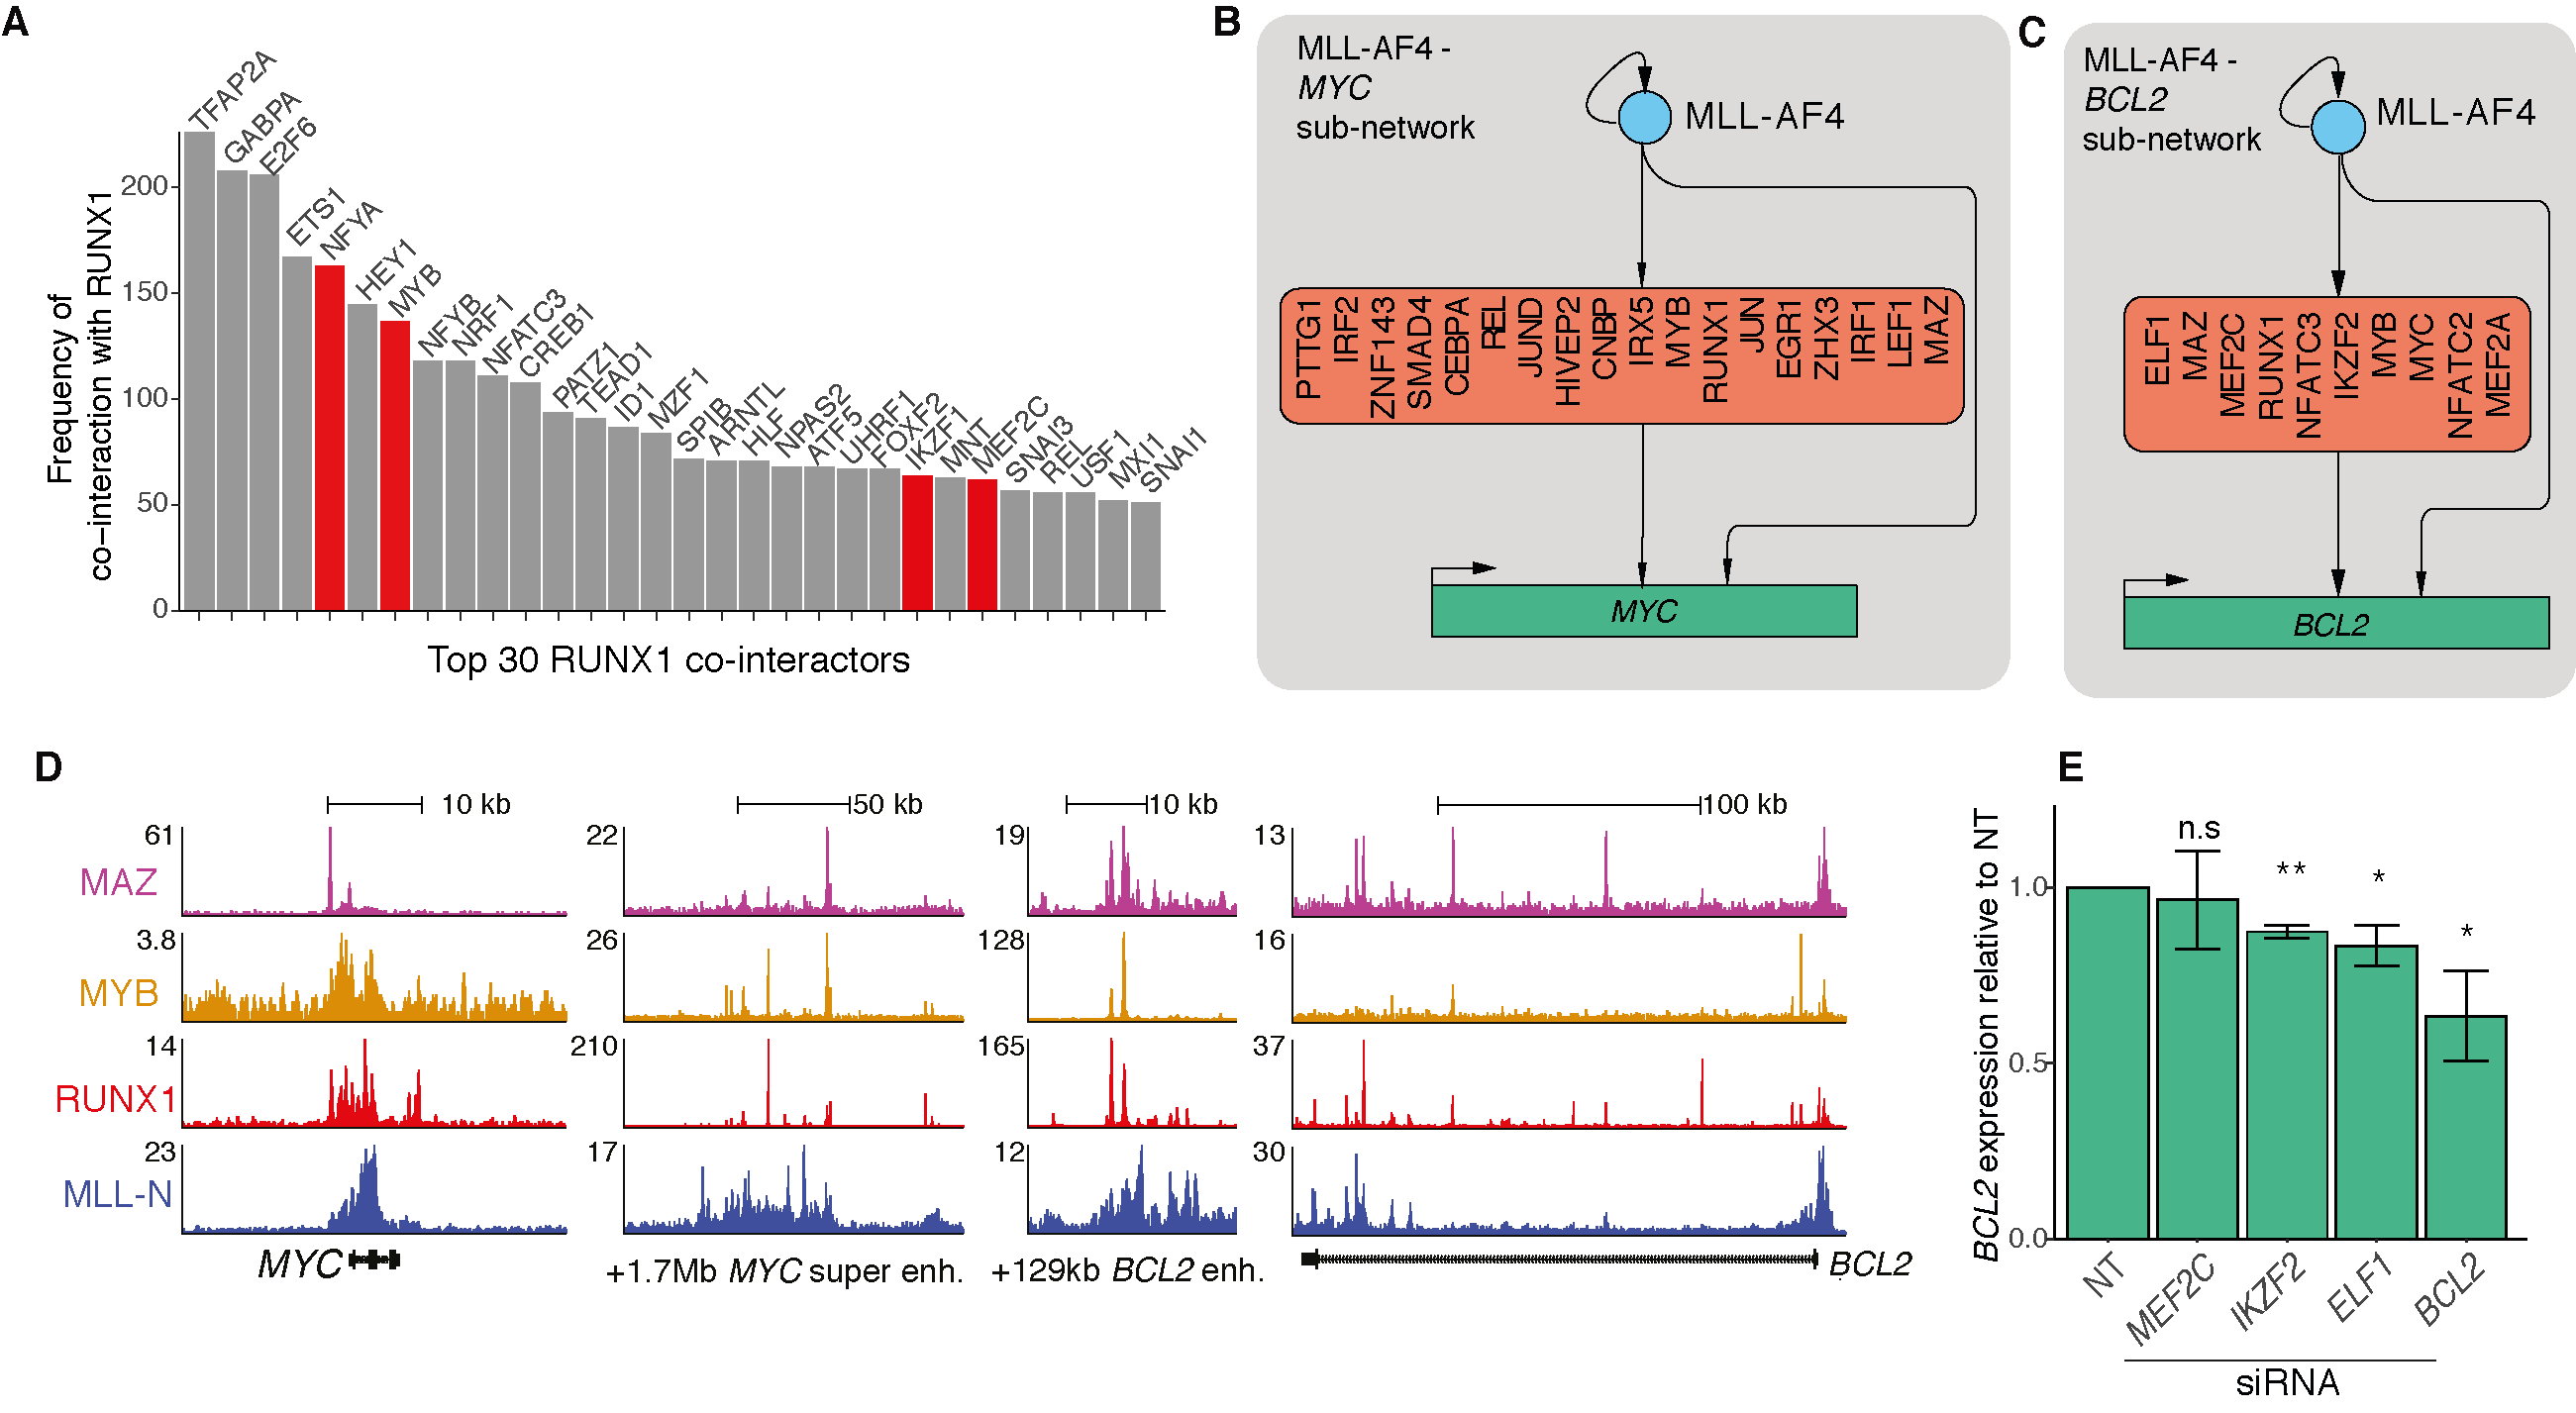
\includegraphics[width=\textwidth,height=\textheight,keepaspectratio]{figures/chapter4/ch4_tf-coop.png}
    %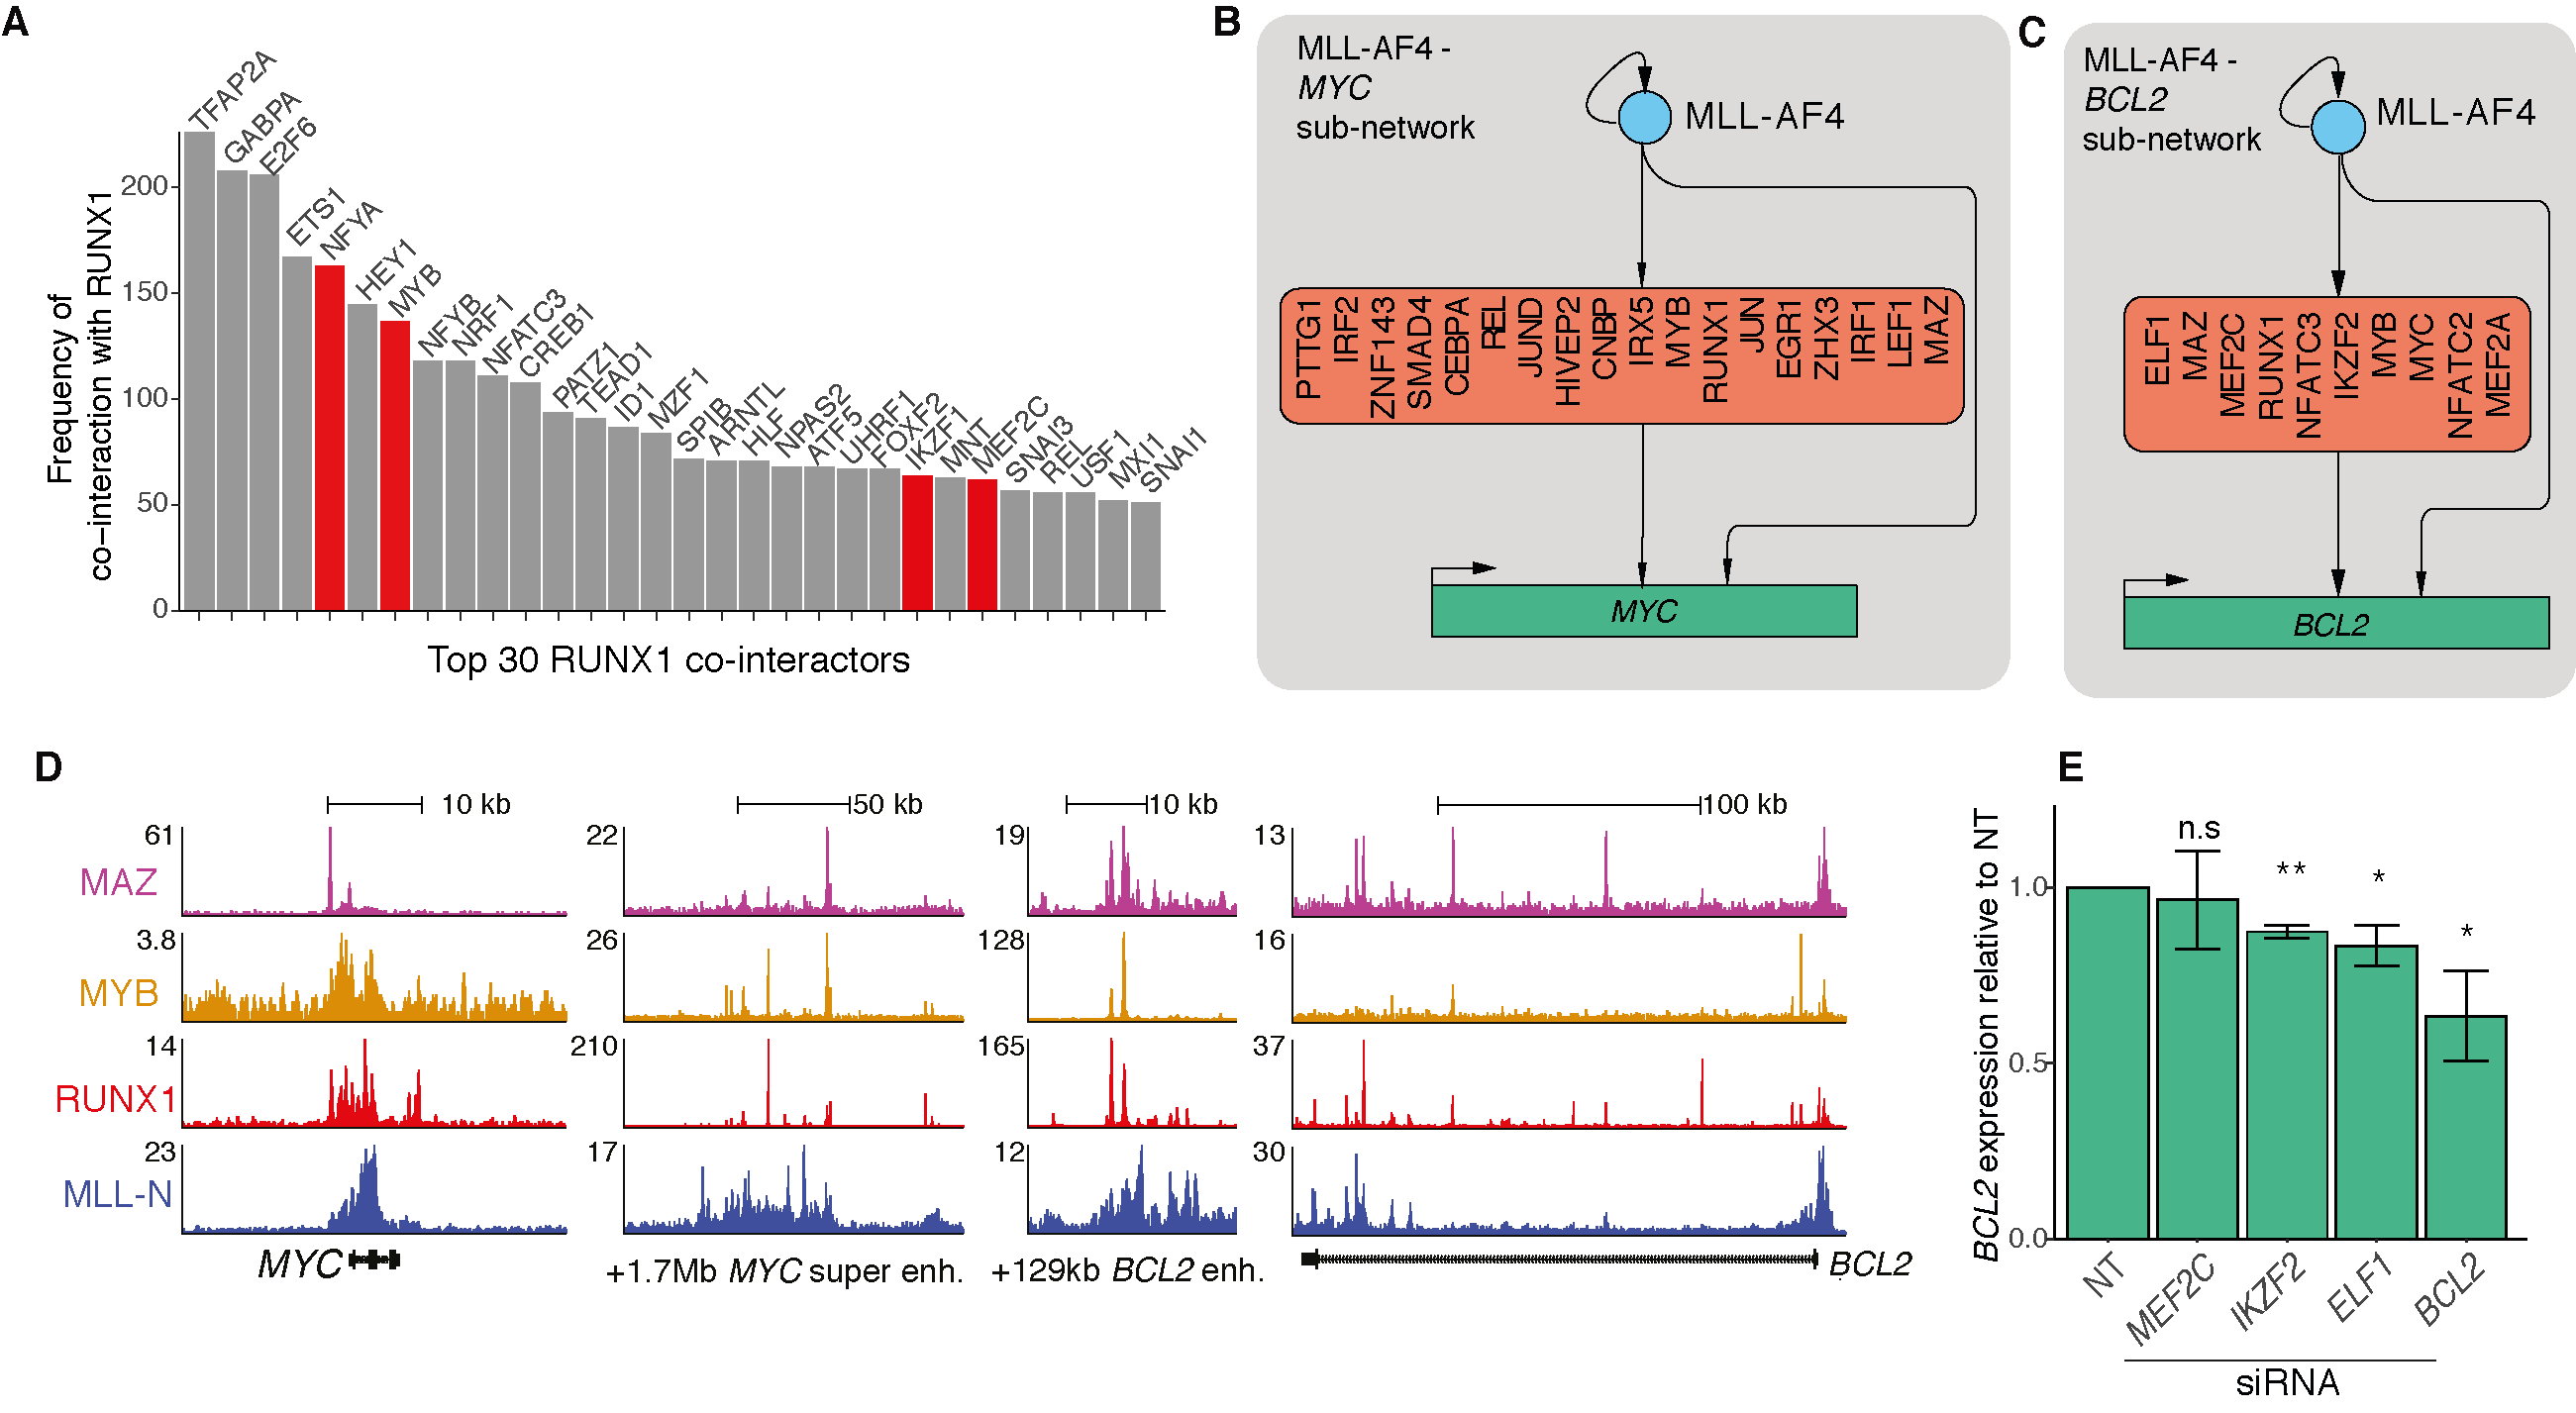
\includegraphics{figures/chapter4/ch4_tf-coop.png}
    \caption[{GRN predicted cooperative regulation of \textit{MYC} and \textit{BCL2}.}]
    {\textbf{GRN predicted cooperative regulation of \textit{MYC} and \textit{BCL2}.} 
    \textbf{(A)} Frequency of TFs co-regulating gene targets with RUNX1. Core MLL-FP TFs highlighted in red. 
    \textbf{(B, C)}  Sub-networks of select interactions from MLL-AF4 and TFs regulating \textit{MYC} (B) and \textit{BCL2} (C). 
    \textbf{(D)} ChIP-seq tracks for MAZ, MYB, RUNX1 and MLL-N at \textit{MYC} and its super enhancer (1.7 Mb downstream of promoter), and \textit{BCL2} and its enhancer (218 kb downstream of promoter). 
    \textbf{(E)} qRT-PCR analysis probing \textit{BCL2} pre-mRNA after 48 h siRNA treatment (\textit{n} = 3). Expression normalized to \textit{GAPDH}, and shown relative to NT control. 
    Bars show mean with standard error; (*) P < 0.05; (**) P < 0.01.
    \textit{Adapted from \cite{harman_kmt2a-aff1_2021}. Myb ChIP-seq data sourced from \citep{godfrey_dot1l_2019}.}
    }
    \label{fig:ch4_tf-coop}
\end{figure}

The most frequent TFs to co-regulate the same genes as RUNX1 include core MLL-FP GRN TFs NF-YA, MYB, IKZF1 and MEF2C (Fig. \ref{fig:ch4_tf-coop}A). Each of these factors also co-interact with Runx1 in EHT (Fig. \ref{fig:ch3_TF-cointeraction}D, p.\pageref{fig:ch3_TF-cointeraction}). Of these factors, MYB is predicted to regulate both \textit{MYC} and \textit{BCL2} along with RUNX1 (Fig. \ref{fig:ch4_tf-coop}B-C). MAZ is a central TF that does not significantly co-interact with RUNX1, yet is predicted to regulate both gene targets. These factors are bound at both loci, the +1.7 Mb \textit{MYC} superenhancer \citep{shi_role_2013}, and a +129 kb \textit{BCL2} enhancer (Fig. \ref{fig:ch4_tf-coop}D). Other central factors predicted to regulate \textit{BCL2} include MEF2C, IKZF2 and ELF1, of which \textit{IKZF2} and \textit{ELF1} KD lowers \textit{BCL2} expression (Fig. \ref{fig:ch4_tf-coop}E), validating these predicted interactions.

\begin{figure}[!t]
    \centering
    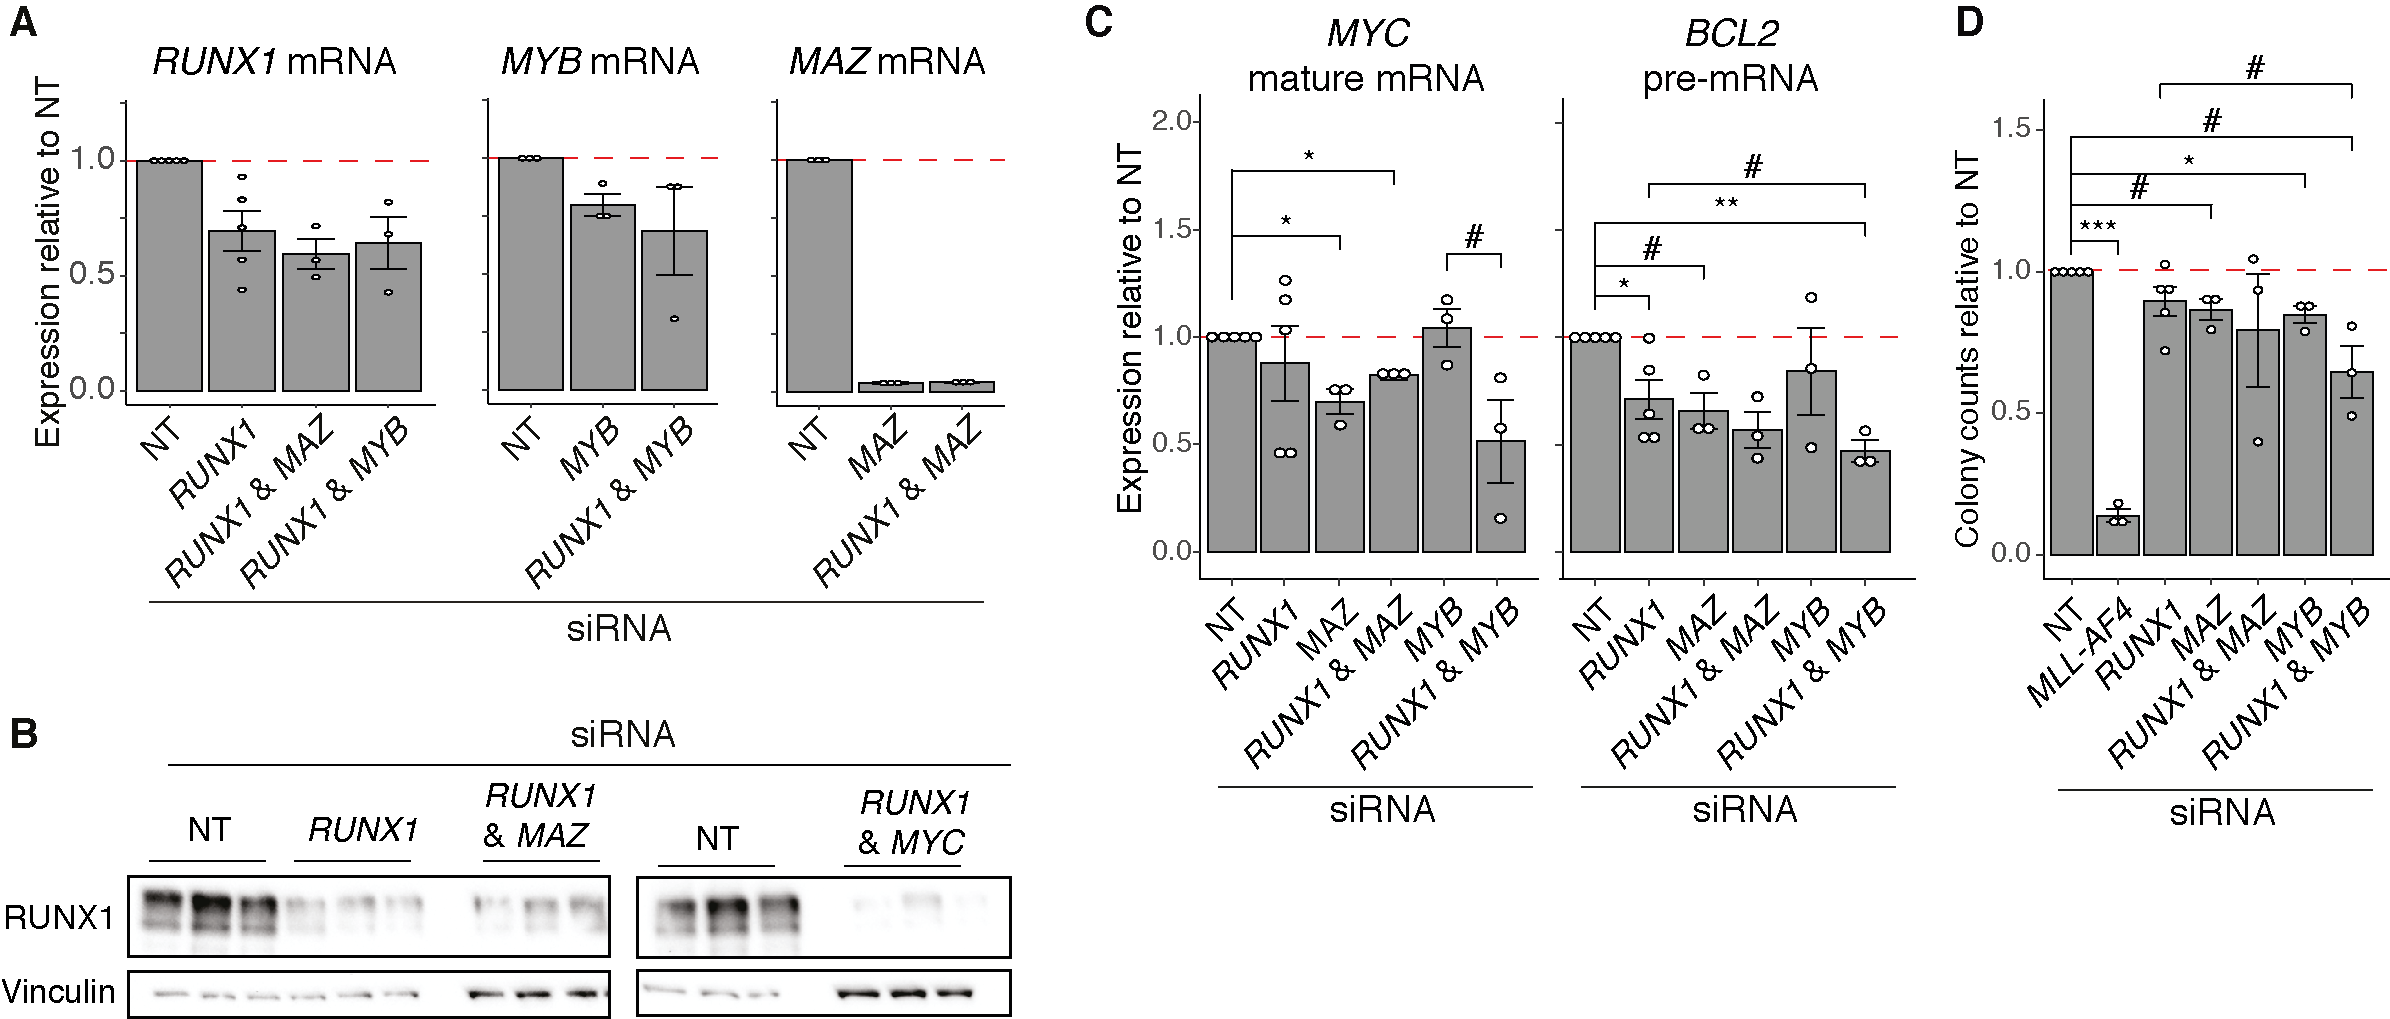
\includegraphics[width=\textwidth,height=\textheight,keepaspectratio]{figures/chapter4/ch4_tf-coop-kd.png}
    %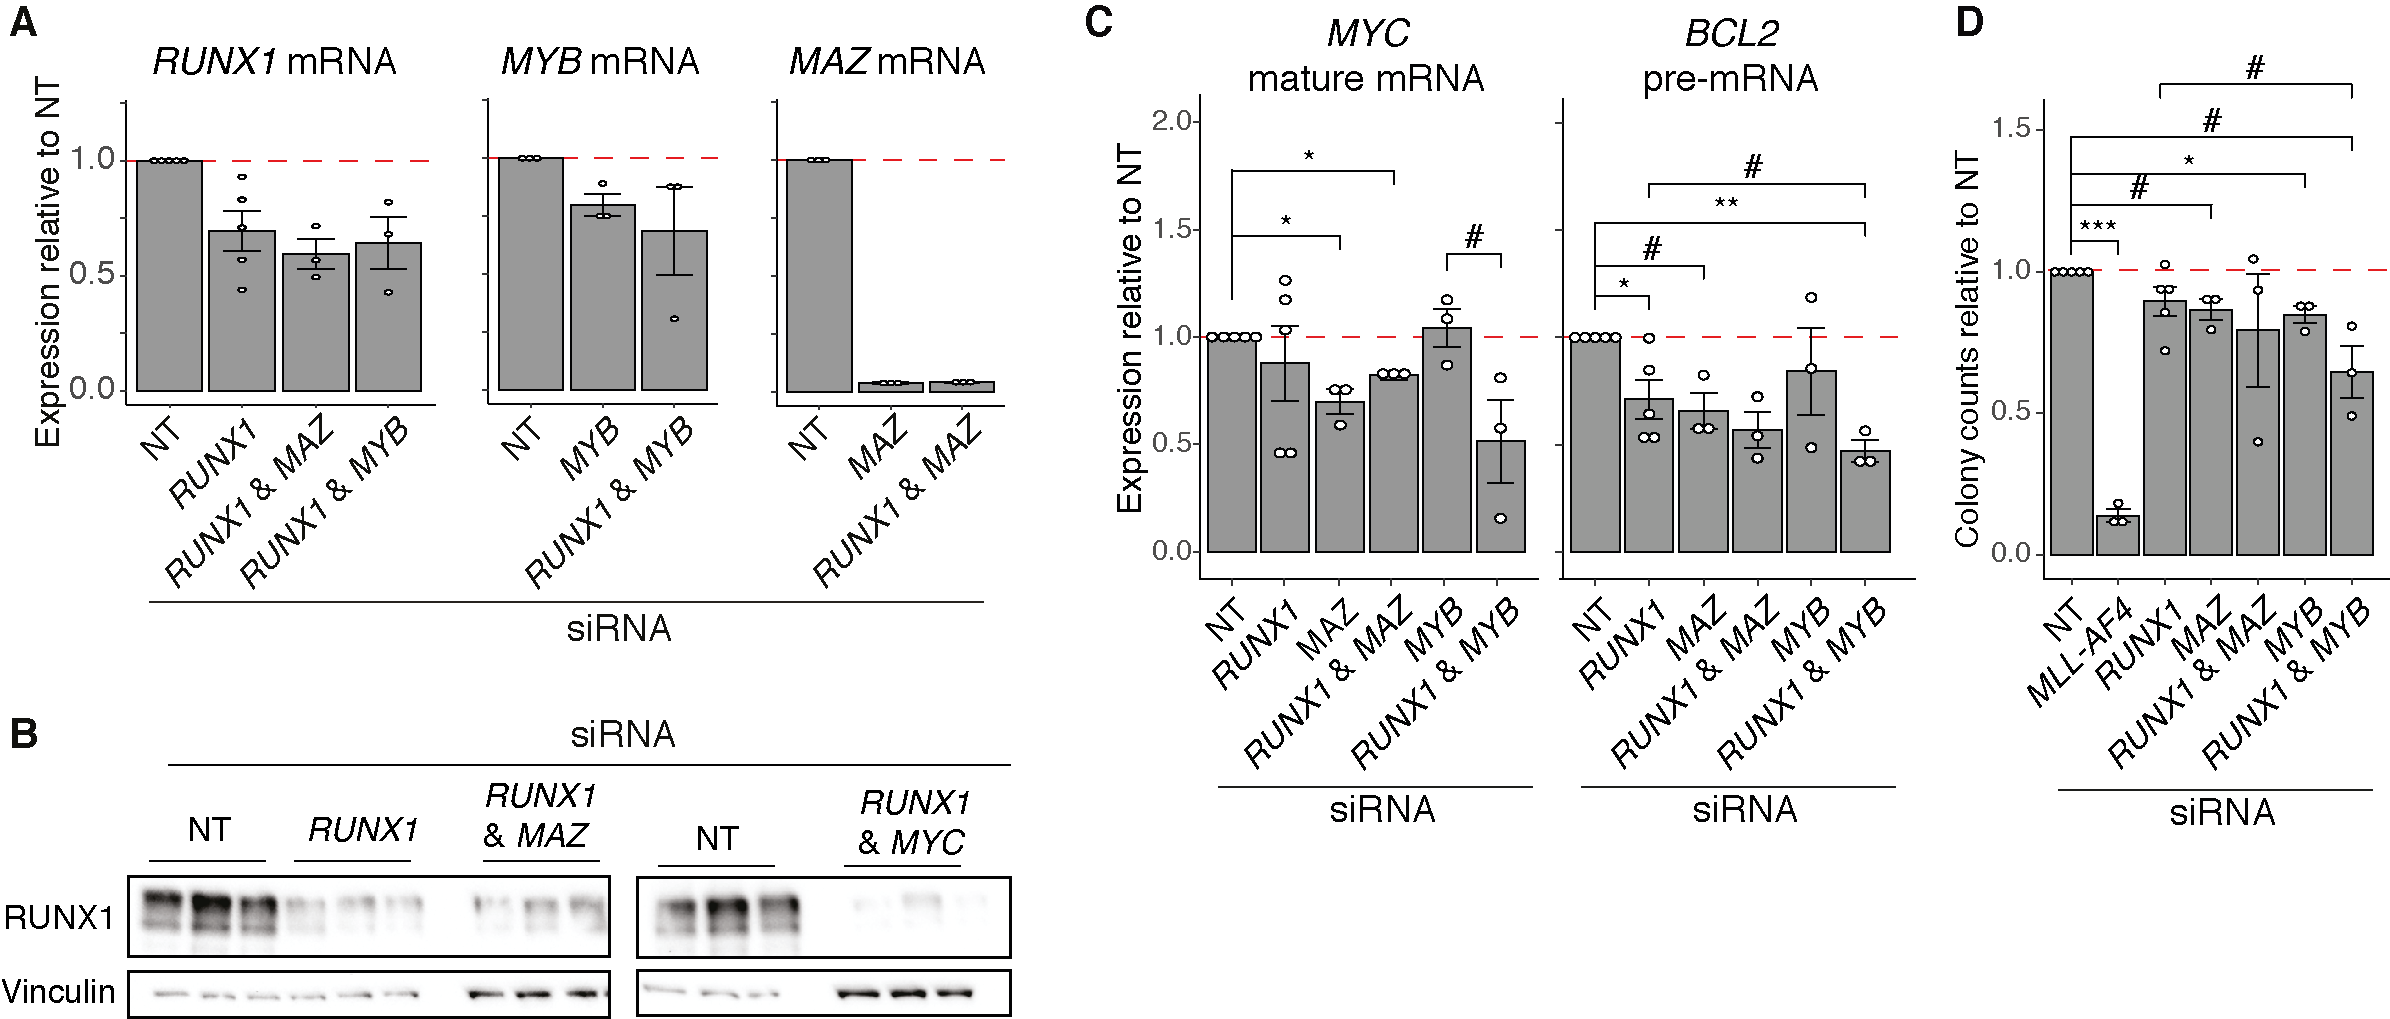
\includegraphics{figures/chapter4/ch4_tf-coop-kd.png}
    \caption[{RUNX1 and MYB cooperate to drive \textit{MYC} and \textit{BCL2} expression.}]
    {\textbf{RUNX1 and MYB cooperate to drive \textit{MYC} and \textit{BCL2} expression.} 
    \textbf{(A)} qRT-PCR analysis for \textit{RUNX1}, \textit{MYB}, and \textit{BCL2} after 96 hours’ siRNA treatment (\textit{n} = 3, \textit{n} = 5 for \textit{RUNX1} KD). Expression normalized to \textit{GAPDH}, and shown relative to NT control. 
    \textbf{(B)} Western blot for RUNX1 after 96 hours’ siRNA treatment as indicated. Vinculin used as loading control. Three replicate experiments are shown. 
    \textbf{(C)} qRT-PCR analysis probing mature \textit{MYC} mRNA and \textit{BCL2} pre-mRNA after 96 h siRNA treatment as indicated (\textit{n} = 3, \textit{n} = 5 for NT and \textit{RUNX1} KD). Expression normalized to \textit{GAPDH}, and shown relative to NT control. 
    \textbf{(D)} Colony forming assay counts after 96 h siRNA treatment as indicated (\textit{n} = 3, \textit{n} = 5 for NT and \textit{RUNX1} KD). Counts shown relative to NT control. 
    Bars show mean with standard error; (\#) P < 0.1; (*) P < 0.05; (**) P < 0.01; (***) P < 0.001.
    \textit{Adapted from \cite{harman_kmt2a-aff1_2021}.}
    }
    \label{fig:ch4_tf-coop-kd}
\end{figure}

I performed KDs of \textit{RUNX1}, \textit{MYB} and \textit{MAZ} alone or in combination with \textit{RUNX1}. Perturbations reduced mRNA and protein levels with no interaction in co-treatments affecting siRNA efficiency (Fig. \ref{fig:ch4_tf-coop-kd}A-B). Due to stability of mature \textit{BCL2} transcripts, intronic primers were used to probe \textit{BCL2} pre-mRNA, as in \cite{crump_bet_2021}. \textit{RUNX1} KD alone was sufficient to reduce \textit{BCL2} expression, but not \textit{MYC} (Fig. \ref{fig:ch4_tf-coop-kd}C). \textit{MAZ} KD significantly reduced \textit{MYC} expression, in line with existing literature \citep{komatsu_maz_1997}, and borderline reduced \textit{BCL2} expression (P = 0.055). \textit{MYB} KD on its own showed no effect. However, combined \textit{RUNX1} and \textit{MYB} KD induced \textit{MYC} and \textit{BCL2} expression to trend towards downregulation, albeit not reaching significance (\textit{MYC} P = 0.09; \textit{BCL2} P = 0.063). \textit{RUNX1} and \textit{MAZ} KD showed no additional effect over individual perturbations. These results suggest that RUNX1 and MAZ function independently at these loci, while RUNX1 and MYB exhibit some level of co-regulation. 

To see whether this cooperation extended to overall leukaemogenesis I used a CFU assay to assess growth following single or double TF KD (Fig. \ref{fig:ch4_tf-coop-kd}D). Note that the concentration of \textit{RUNX1} siRNA used was lower than in \cite{wilkinson_runx1_2013}, so \textit{RUNX1} KD RNA was incompletely perturbed (Fig. \ref{fig:ch4_tf-coop-kd}A-B) and resulted in minimal growth impact. \textit{MAZ} KD on its own slightly reduced colony forming potential (P = 0.075), but additional \textit{RUNX1} perturbation did not enhance this. \textit{MYB} KD significantly impacted growth, and when combined with \textit{RUNX1} KD the effect was increased though not reaching significance (P = 0.091). These assays further suggest that not only do RUNX1 and MYB co-interact to regulate \textit{MYC} and \textit{BCL2}, but they also function to promote leukaemogenesis. Integrating these results together begins to interrogate the possible TF co-interaction at key loci, and provides a template for further study into gene regulation in leukaemia.

\section{\label{ch4:multiome}MLL-AF4 and cooperative TFs co-opt and drive normal fetal circuits.}

I have established that MLL-AF4 and RUNX1 function cooperatively at many loci, and that TF cooperation drives key target expression. MLL-AF4 and RUNX1 regulatory logic also overlapped at B cell differentiation processes (Fig. \ref{fig:ch4_interplay}B). \textit{MLL} rearrangements in infant ALL (iALL) are thought to occur in fetal life \citep{greaves_causal_2018, greaves_utero_2005, ford_utero_1993, jackson_origin_2021}, consistent with the observation that \textit{MLL}r leukaemias are associated with overexpressed fetal programs \citep{rice_human_2021}, and the MLL-AF4 GRN contains active FBM modules (Fig. \ref{fig:ch4_patient}). Thus, it is possible MLL-AF4 directly co-opts fetal TFs and pathways. To address whether normal fetal circuits are overactivated by the MLL-AF4 GRN, we collaborated with the Roy lab to generate single cell RNA+ATAC multiome (sc-multiome) data, profiling healthy CD34+ (stem and progenitor cells) and CD34- FBM and fetal liver (FL) cells from healthy donors. In addition, we profiled iALL and childhood ALL (chALL) blasts from patients, alongside xenograft models of MLL-AF4 transformed CD34+ FL cells generated by S. Rice using CRISPR induced translocation \citep{rice_human_2021} (Table \ref{tbl:ch4_multiome-samples}). Samples were pooled in male-female pairs, and demultiplexed using a combination of \textit{XIST} and Y chromosome expression and clustering of single cell variant calls (methods section \ref{ch2:single-cell}, p.\pageref{ch2:single-cell}). High quality, robustly deconvoluted cells were retained, and two samples (iALL-X and chALL-X) were discarded for poor cell capture (Table \ref{tbl:ch4_multiome-samples}, Appendix \ref{fig:app_multiome-qc}A-C).

\begin{table}[htbp]
\caption{Patient and healthy donor samples used for single cell RNA+ATAC multiome analysis}
\resizebox{\textwidth}{!}{
\begin{tabular}{@{}llllllll@{}}
\toprule
ID & Population & Gender & Well & Cells pre-QC & Cells post-QC & Notes \\ \midrule
FBM1.1 & CD34- FBM & Male & 1 & 3836 & 3146 &  \\
FBM2.1 & CD34- FBM & Female & 1 & 3810 & 2966 &  \\
FBM1.2 & CD34+ FBM & Male & 2 & 3748 & 3359 &  \\
FBM2.2 & CD34+ FBM & Female & 2 & 3123 & 2567 &  \\
FL1.1 & CD34- FL & Male & 3 & 3276 & 2736 &  \\
FL2.1 & CD34- FL & Female & 3 & 3165 & 2611 &  \\
FL1.2 & CD34+ FL & Male & 4 & 3129 & 2735 &  \\
FL2.2 & CD34+ FL & Female & 4 & 4998 & 4180 &  \\
iALL2 & iALL blasts & Male & 5 & 3901 & 3518 &  \\
iALL1 & iALL blasts & Female & 5 & 3653 & 2868 &  \\
iALL3 & iALL blasts & Male & 6 & 5435 & 4526 &  \\
chALL & chALL blasts & Male & 6 & 5755 & 5160 &  \\
chALL-X & chALL blasts & Male & 7 & 474 & 30 & Fail \\
iALL-X & iALL blasts & Female & 7 & 595 & 350 & Fail \\
Xeno2-1 & xenoALL blasts & Male & 8 & 2856 & 2512 &  \\
Xeno3-3 & xenoALL blasts & Female & 8 & 3018 & 2724 &  \\
Xeno2-2 & xenoALL blasts & Male & 9 & 4994 & 4530 &  \\
Xeno3-2 & xenoALL blasts & Female & 9 & 6196 & 5752 &  \\
Failed deconvolution &  &  &  & 8841 &  &  \\ \bottomrule
\end{tabular}
}
\label{tbl:ch4_multiome-samples}
\end{table}

The MLL-AF4 GRN is based on SEM cells, a B-cell ALL cell line. As such, I aimed to isolate HSPCs and B progenitors to capture the B lineage. To identify cell types, FBM/FL samples and MLL-AF4 ALL blasts were clustered, incorporating both RNA expression and chromatin accessibility profiles (methods section \ref{ch2:single-cell}, p.\pageref{ch2:single-cell}, \cite{hao_integrated_2021}). Cells were annotated by label transfer using reference datasets \citep{popescu_decoding_2019, jardine_blood_2021, roy_transitions_2021}, and the B-cell lineage was manually curated using known transcriptional markers (Fig. \ref{fig:ch4_multiome-clusters}A-B, Appendix \ref{fig:app_multiome-lineage-markers}, \cite{jardine_blood_2021, suo_mapping_2022}). 

\begin{figure}[!t]
    \centering
    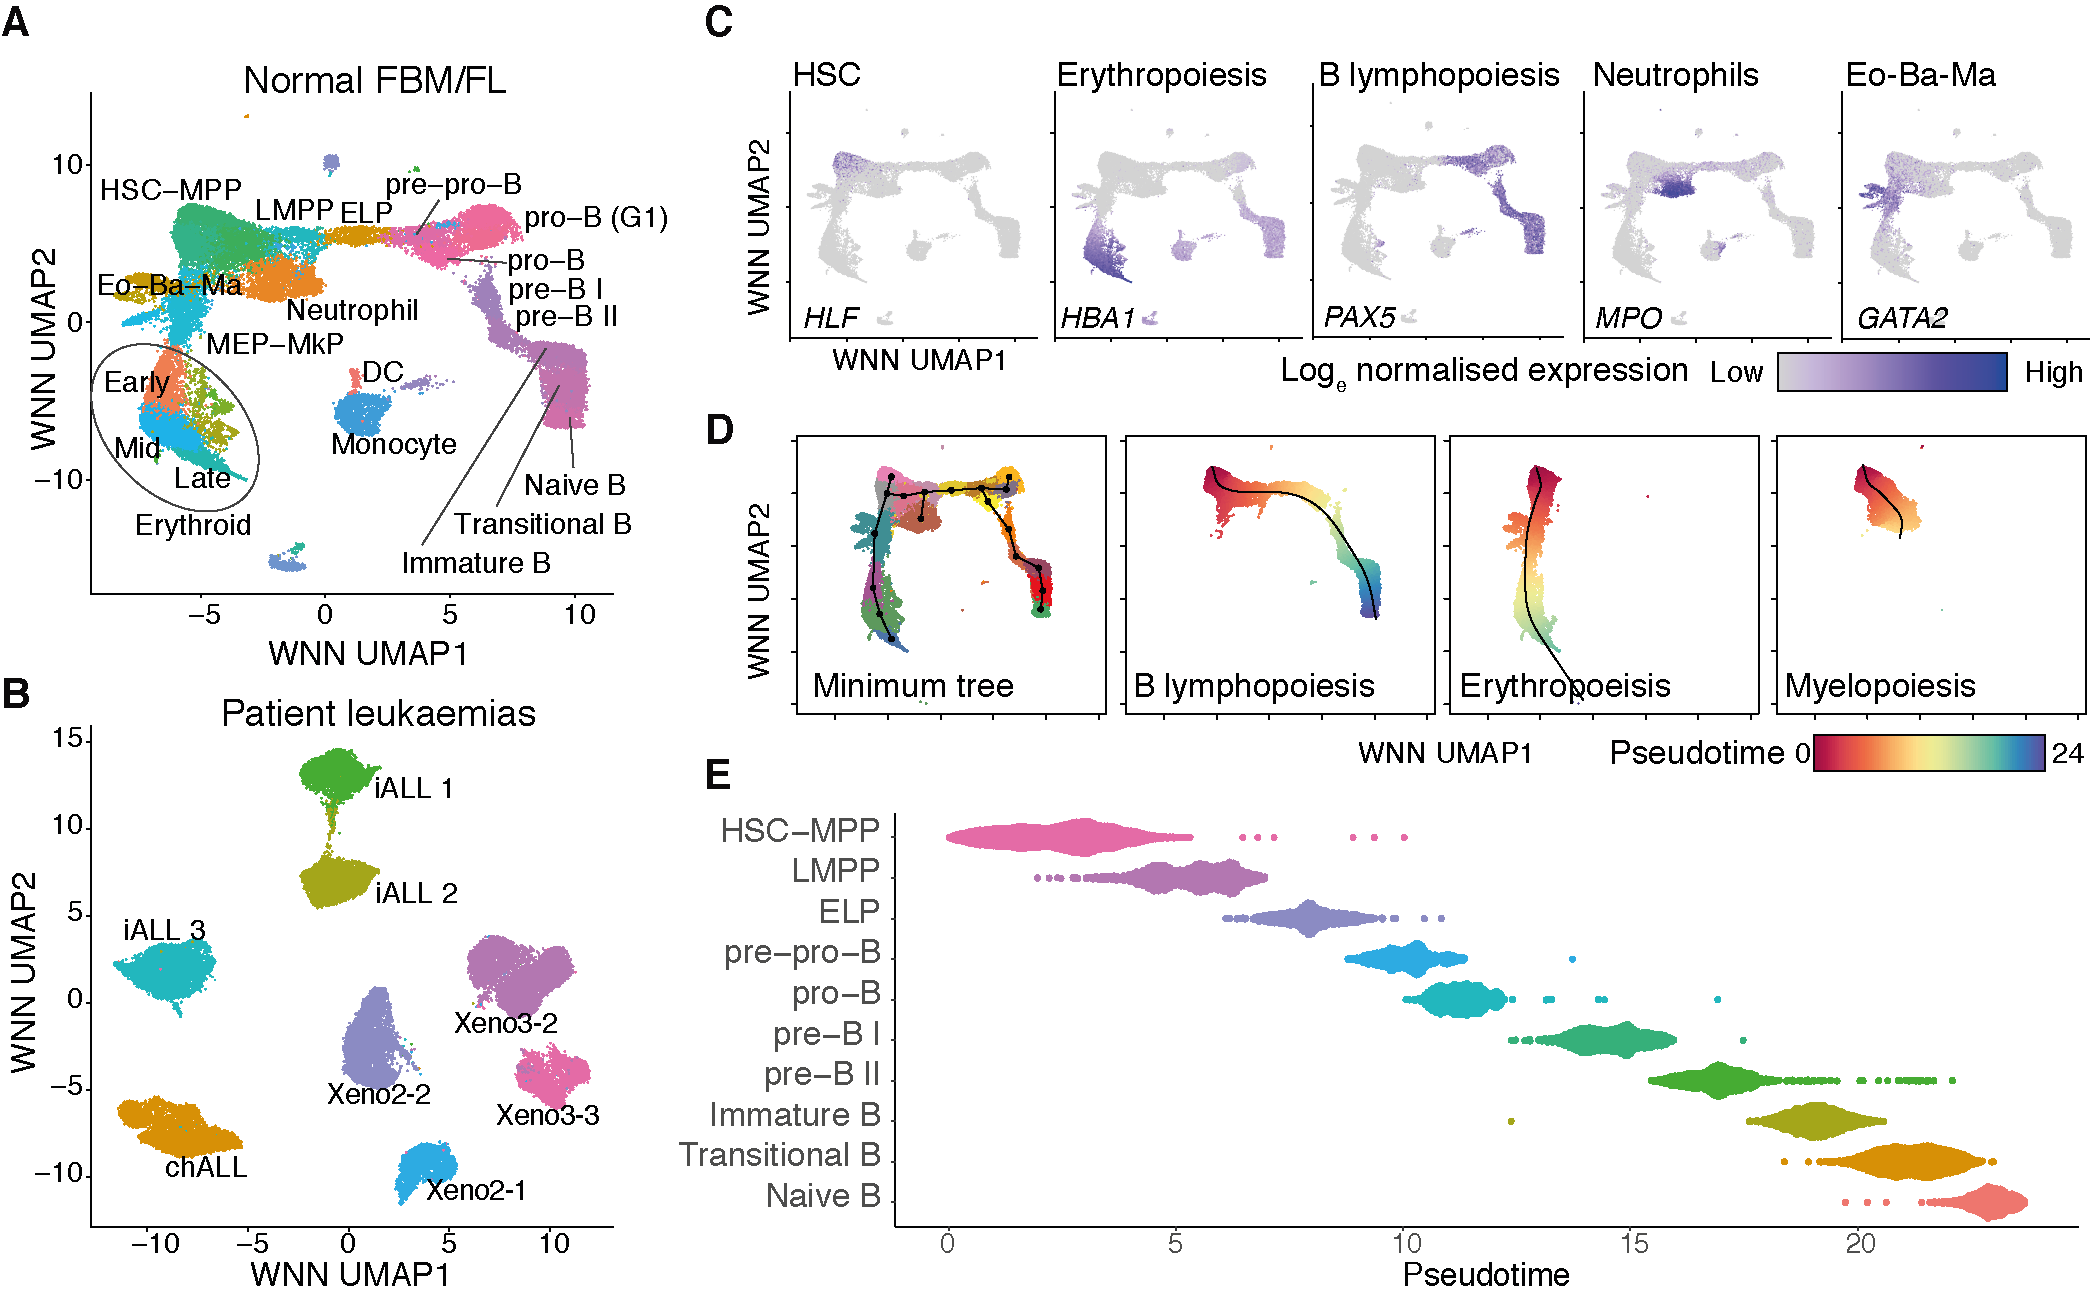
\includegraphics[width=\textwidth,height=\textheight,keepaspectratio]{figures/chapter4/ch4_multiome-clusters.png}
    \caption[{Sc-multiome trajectory analysis of  FBM and FL cells recapitulates three fetal lineages.}]
    {\textbf{Sc-multiome trajectory analysis of  FBM and FL cells recapitulates three fetal lineages.} 
    \textbf{(A, B)} UMAP dimensionality reduction and clustering performed using RNA+ATAC WNN graphs for normal FBM and FL cells (A), and patient and xenograft ALL blasts (B). Cluster identities annotated.
    \textbf{(C)} Expression of key lineage defining markers.
    \textbf{(D)} Lineage assignment through slingshot trajectory analysis, using HSC-MPP cluster as the lineage start.
    \textbf{(E)} B lymphopoiesis assigned cells ordered by slingshot pseudotime, stratified by assigned cluster as in A. 
    \textit{Analysis of the sc-multiome was performed by me in collaboration with A. Smith (scATAC-seq pre-processing).}
    }
    \label{fig:ch4_multiome-clusters}
\end{figure}

Rather than focusing on individual clusters, I opted for a pseudotime approach to interrogate lineages, which allows for identification of expression patterns and quantitative changes in gene expression rather than cluster-dependent classification of marker genes. Slingshot trajectory analysis grouped cells into three lineages originating from HSCs (Defined by \textit{HLF} expression, \cite{lehnertz_hlf_2021}), including erythropoiesis (\textit{HBA1}), myelopoiesis/neutrophils (\textit{MPO}, \cite{aratani_myeloperoxidase_2018}), and B lymphopoiesis (\textit{PAX5}, \cite{nutt_pax5_2001}) (Fig. \ref{fig:ch4_multiome-clusters}C-D). As a computational artifact the erythropoiesis lineage also picks up an eosinophil/basophil/mast cluster (Eo-Ba-Ma, \textit{GATA2}, \cite{ohmori_gata2_2015}). Pseudotime ordering of these lineages organises cells into sequential clusters, from HSPCs through to mature populations (Fig. \ref{fig:ch4_multiome-clusters}E, Appendix \ref{fig:app_multiome-other-pseudo}).

\begin{figure}[p]
    \centering
    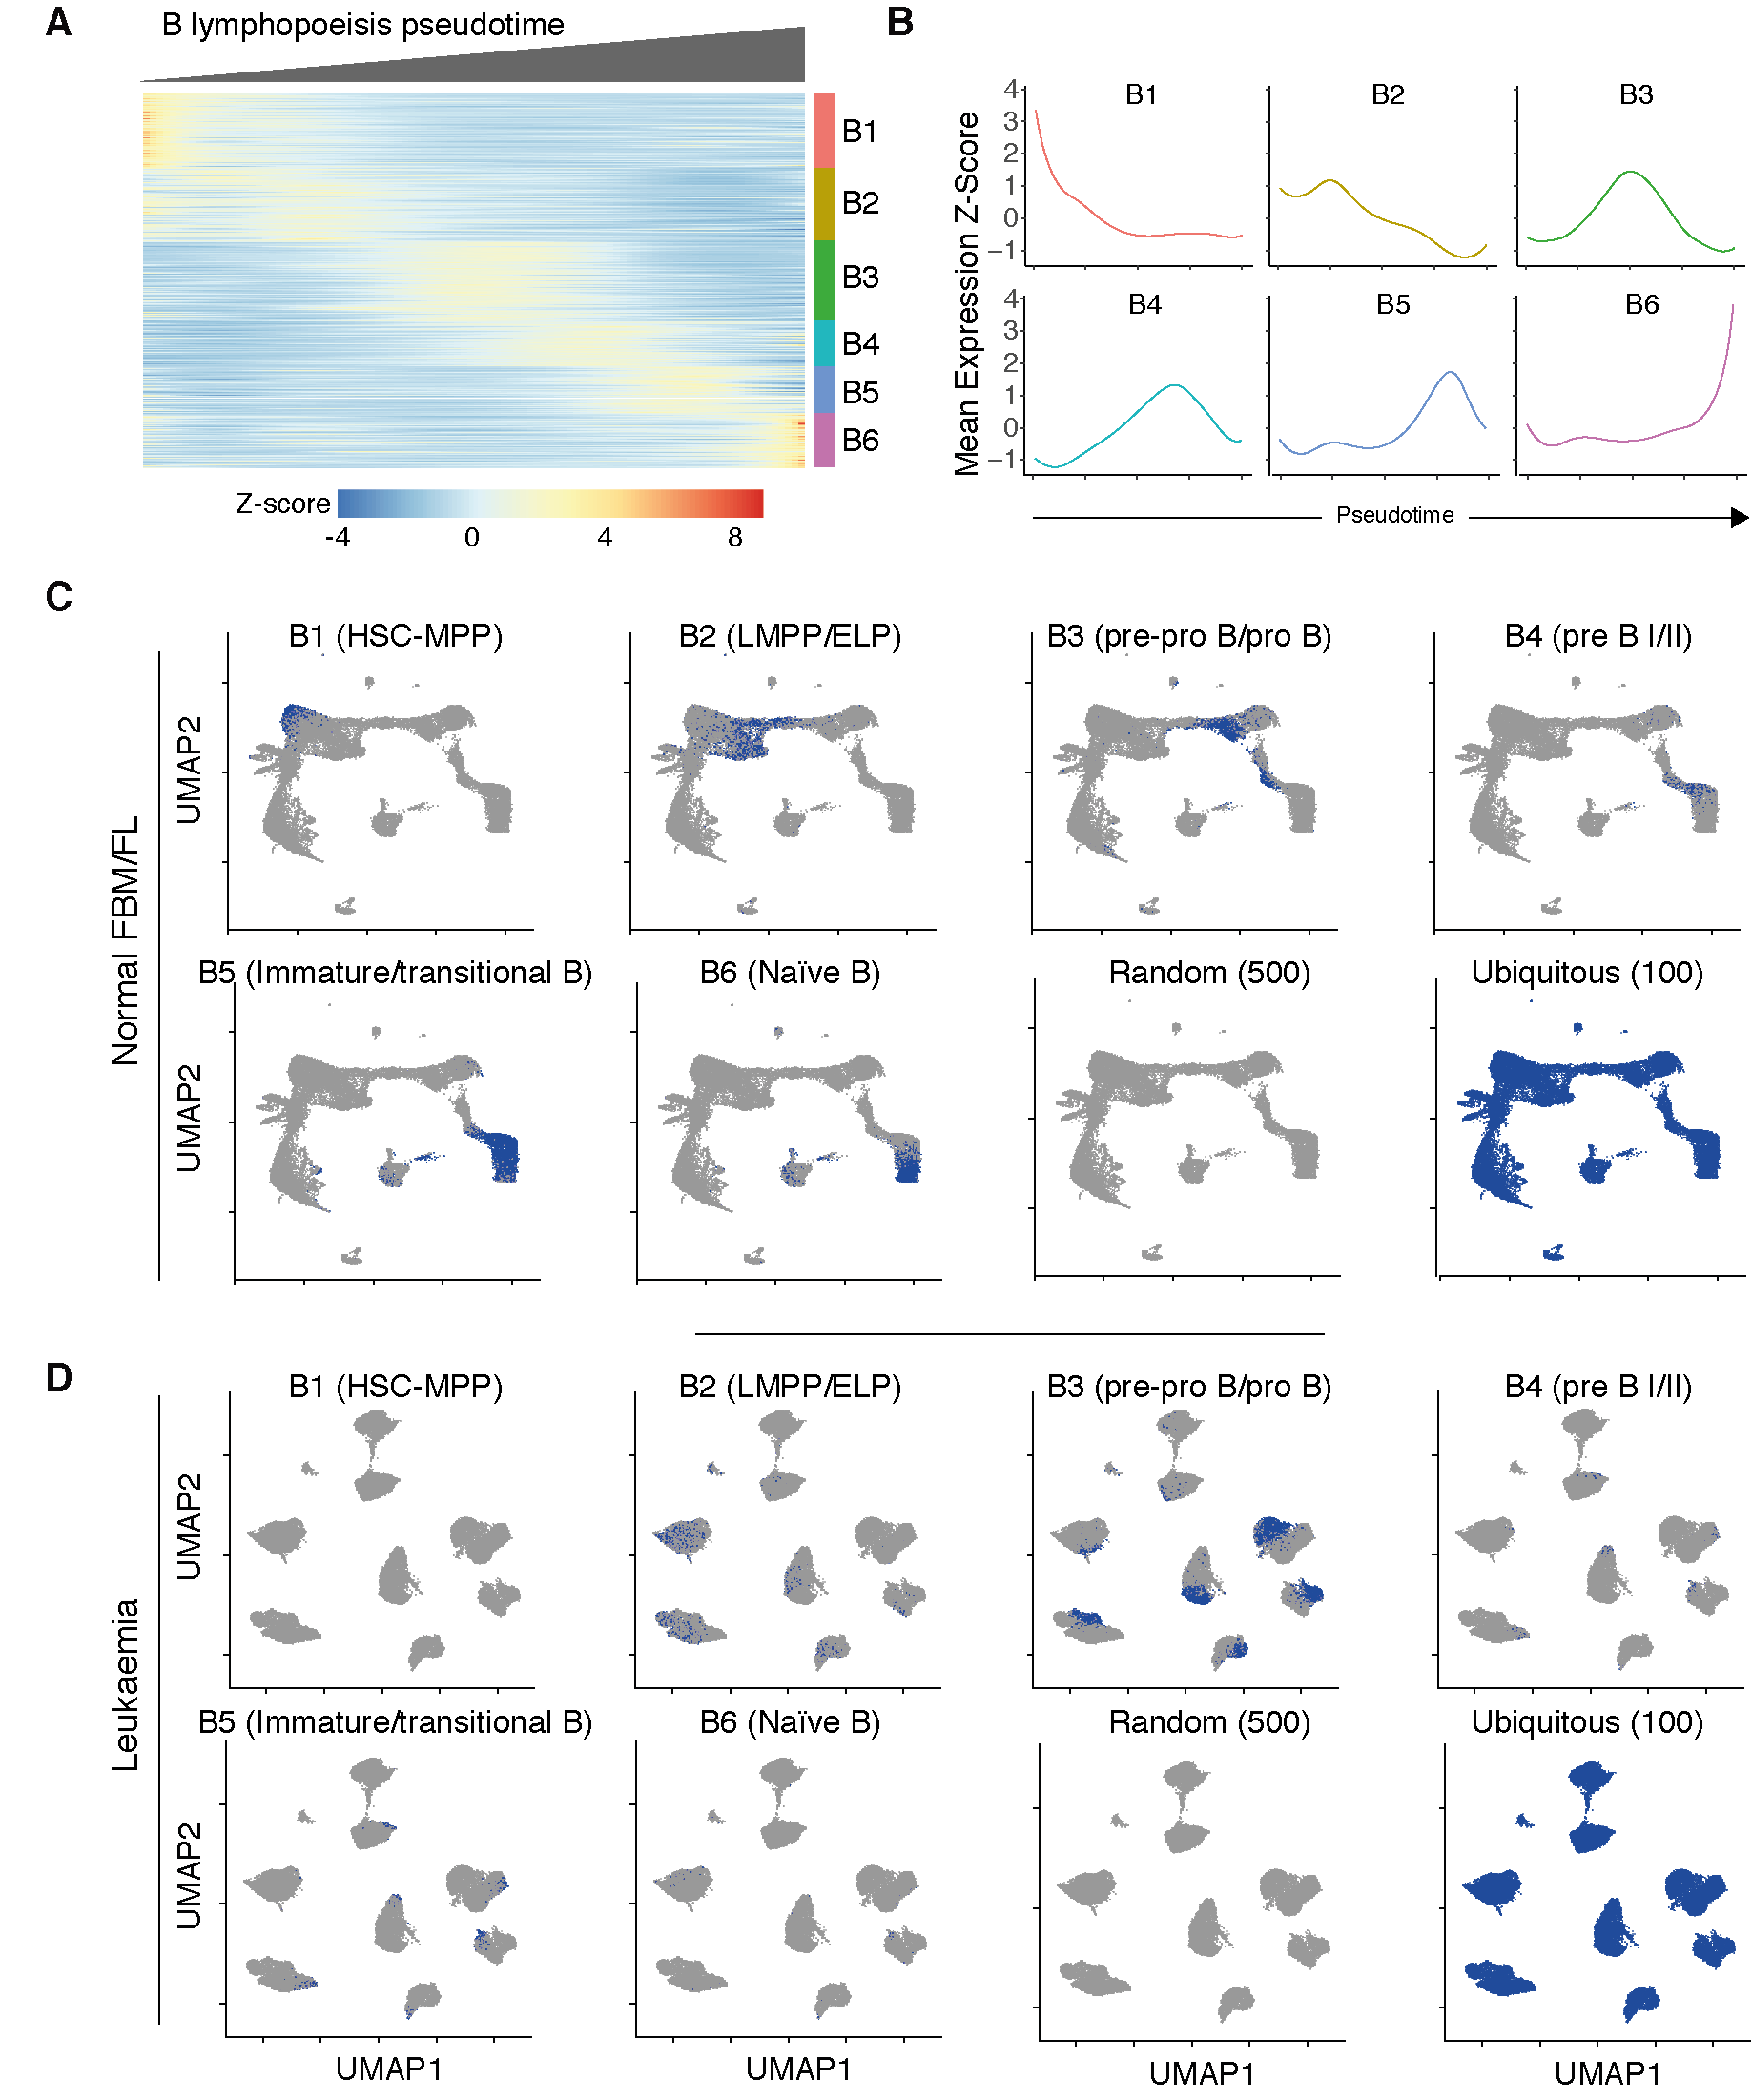
\includegraphics[width=\textwidth,height=\textheight,keepaspectratio]{figures/chapter4/ch4_multiome-tradeseq.png}
    \caption[{pre-pro-B/pro-B biased B-lymphopoiesis associated genes are enriched in MLL-AF4 ALL blasts.}]
    {\textbf{pre-pro-B/pro-B biased B-lymphopoiesis associated genes are enriched in MLL-AF4 ALL blasts.} 
    \textbf{(A)} Heatmap of z-score expression, smoothed over pseudotime into 100 bins, with genes as rows and cells as columns ordered by B lymphopoiesis pseudotime. \textit{k}-means clusters (B lymphopoiesis signatures) shown on the side.
    \textbf{(B)} Average z-score expression, smoothed over pseudotime into 100 bins, split by clusters as in A.
    \textbf{(C-D)} FL and FBM (C) or ALL blast (D) UMAPs, with datapoints coloured blue for cells passing AUCell thresholds, marking enrichment for signatures as in A-B. The same thresholds were used for each signature between FBM/FL and ALL blasts. Random and ubiquitous gene sets are shown as controls.
    }
    \label{fig:ch4_multiome-tradeseq}
\end{figure}


Differential analyses for expression changes over pseudotime was performed to generate a panel of B lineage associated genes (methods section \ref{ch2:pseudo}, p.\pageref{ch2:pseudo}), which were clustered into six B lymphopoiesis signatures (B1-6, Fig. \ref{fig:ch4_multiome-tradeseq}A-B). As determined by single cell signature enrichment (AUcell), these map to HSC-MPP (B1), LMPP/ELP (B2), pre-pro-B/pro-B (B3), pre-B I and II (B4), immature/transitional B (B5) and Na\"{i}ve B (B6) cells (Fig. \ref{fig:ch4_multiome-tradeseq}C). To investigate how ALL gene expression compared with normal B lymphopoiesis expression, I probed the ALL samples with the B lymphopoiesis signatures. Interestingly only signatures pre-pro-B/pro-B (B3), and to a lesser extent LMPP/ELP (B2), were enriched in the iALL and chALL blasts (Fig. \ref{fig:ch4_multiome-tradeseq}D). This suggests that ALL blasts maintain transcriptional profiles from LMPP through to pro-B, but not more differentiated B lineage populations.

\begin{figure}[!t]
    \centering
    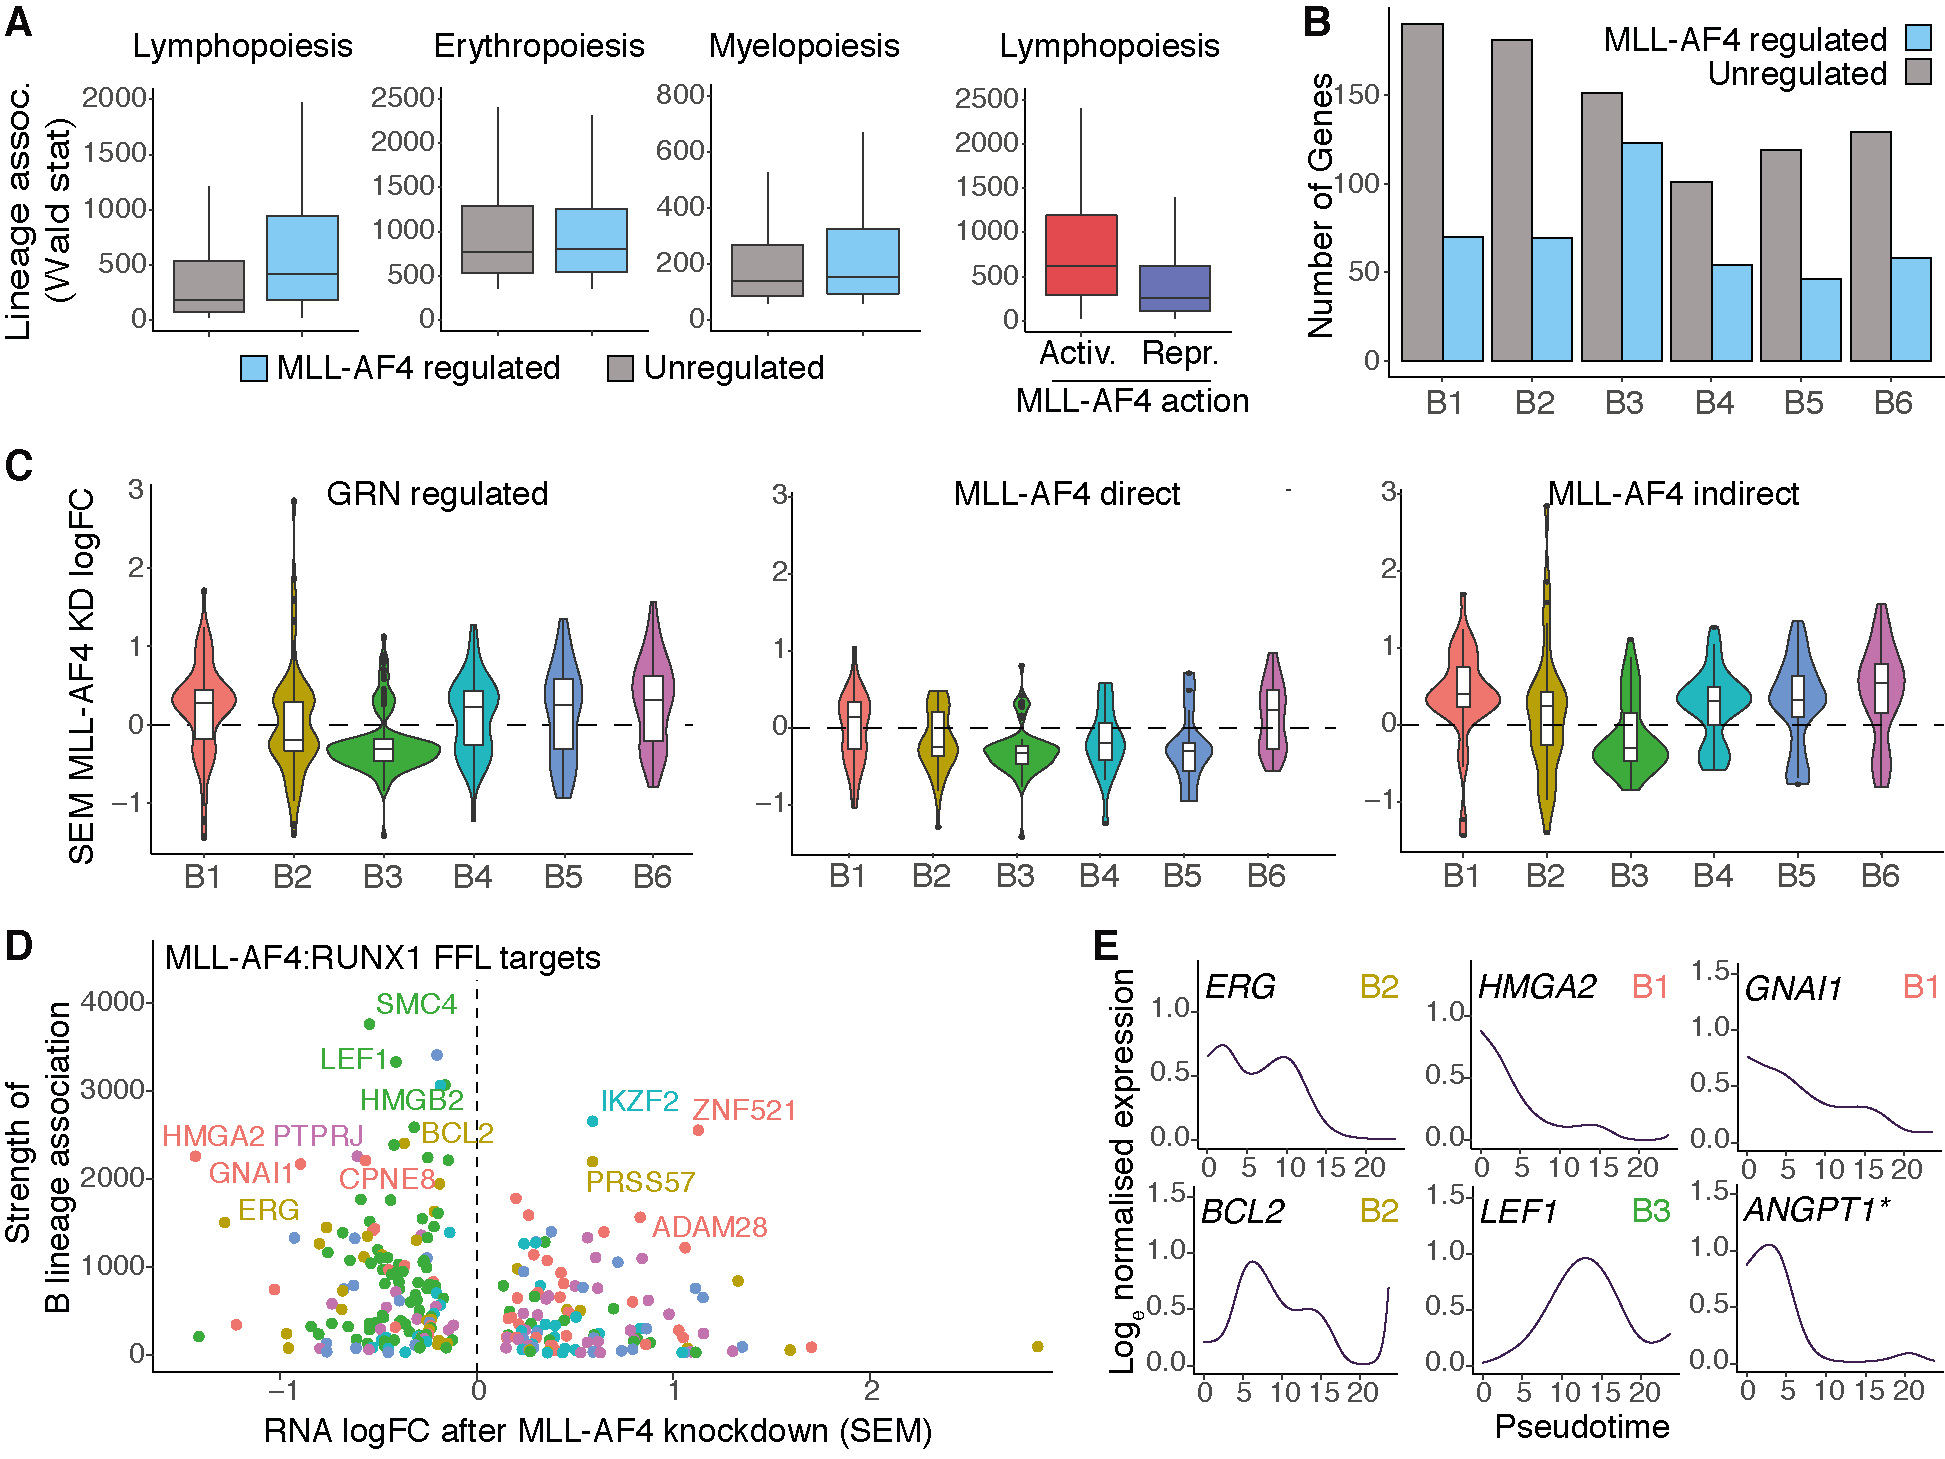
\includegraphics[width=\textwidth,height=\textheight,keepaspectratio]{figures/chapter4/ch4_multiome-grn.png}
    \caption[{The MLL-AF4 GRN drives activation of pre-pro-B/pro-B biased genes, and may repress mature B-cell circuits.}]
    {\textbf{The MLL-AF4 GRN drives activation of pre-pro-B/pro-B biased genes, and may repress mature B-cell circuits.} 
    \textbf{(A)} Distribution of TradeSeq Wald statistics of lineage association for genes expressed in different lineages, split by MLL-AF4 GRN regulation status (left) or whether MLL-AF4 is activating or repressing, as determined in Fig. \ref{fig:ch4_motifs} (right).
    \textbf{(B)} Number of genes associated with each B lymphopoiesis signature, split by MLL-AF4 GRN regulation status.
    \textbf{(C)} Distribution of SEM RNA logFC following 96 hours' \textit{MLL-AF4} KD across B lymphopoiesis signatures at all GRN regulated genes, MLL-AF4 directly, and indirectly regulated genes. 
    \textbf{(D)} Relationship between SEM RNA logFC following 96 hours' \textit{MLL-AF4} KD and TradeSeq Wald statistic of lineage association for B lymphopoiesis. MLL-AF4:RUNX1 FFL motif targets shown. Genes coloured according to B lymphopoiesis signatures.
    \textbf{(E)} TradeSeq smoothed expression plots for select genes in D, that are associated with B lymphopoiesis pseudotime. * Indicates genes were instead detected by pairwise differential expression between HSC and pro-B cells.
    }
    \label{fig:ch4_multiome-grn}
\end{figure}

To determine whether MLL-AF4 co-opts B lymphopoiesis circuits I integrated the MLL-AF4 GRN with the B lymphopoiesis signatures. MLL-AF4 regulated genes were more significantly associated with B lymphopoiesis over non-MLL-AF4 regulated genes, but this was not observed for erythropoiesis or myelopoiesis (neutrophils) (Fig. \ref{fig:ch4_multiome-grn}A). This aligns with the hypothesis that MLL-AF4 drives B progenitor circuits. It is worth noting that while the patient expression data integration in section \ref{ch4:patient-modules} identified a set of core nodes common across leukaemias, this was based on binary transcription and not levels of expression, and it also identified an ALL-specific program. In integrating the MLL-AF4 GRN with B lymphopoiesis signatures this analysis captures this ALL-specific program. Using the SEM \textit{MLL-AF4} KD logFC data to assign activating and repressing interactions (as in Fig. \ref{fig:ch4_motifs}), MLL-AF4 activated genes showed much greater B lymphopoiesis association than MLL-AF4 repressed genes (Fig. \ref{fig:ch4_multiome-grn}A). Strikingly, the GRN interfaces primarily with the B3 (pre-pro-B/pro-B) signature, and upon \textit{MLL-AF4} KD this signature, unlike others, is almost entirely downregulated (Fig. \ref{fig:ch4_multiome-grn}B-C). Distinguishing MLL-AF4 direct and indirect binding reveals that most directly bound genes within each signature are downregulated upon KD, whereas indirectly regulated signatures are upregulated except for B3 (Fig. \ref{fig:ch4_multiome-grn}C). This can be interpreted as MLL-AF4 strongly activating a pre-pro-B/pro-B gene signature, both in the direct and indirect GRN, yet the indirect GRN may drive repression of stem and mature signatures. 

A number of B lymphopoiesis associated genes are regulated by an MLL-AF4:RUNX1 driven FFL (Fig. \ref{fig:ch4_multiome-grn}D). Several FFL targets are associated with B lymphopoiesis, and are strongly regulated by MLL-AF4 (Fig. \ref{fig:ch4_multiome-grn}D-E). These include the key MLL-AF4 target \textit{BCL2}, which shows a B2 expression pattern (ELP/LMPP). \textit{LEF1} is a pre-pro-B/pro-B expressed gene that is a target of MLL-AF4 \citep{kerry_mll-af4_2017} and has a known role in driving pro-B proliferation as a part of WNT signalling \citep{reya_wnt_2000}. \textit{Lef1} was also highlighted in Maf:Lef1:EMT FFLs in mouse EHT (Fig. \ref{fig:ch3_maf1-lef1}). One interesting hypothesis is that MLL-AF4 drives the reactivation of stem and progenitor programs, as seen with the overexpression of \textit{PROM1} \citep{godfrey_h3k79me23_2021, mak_mixed_2012, obyrne_discovery_2019}. In line with this, we find \textit{HMGA2} and \textit{GNAI1} matching a HSC-MPP signature (B1), and \textit{ANGPT1}, which is not part of a signature but was instead identified by pairwise differential expression analysis between HSC-MPP and pro-B clusters. This could reflect reactivation or forced maintenance of these loci. 

\begin{figure}[p]
    \centering
    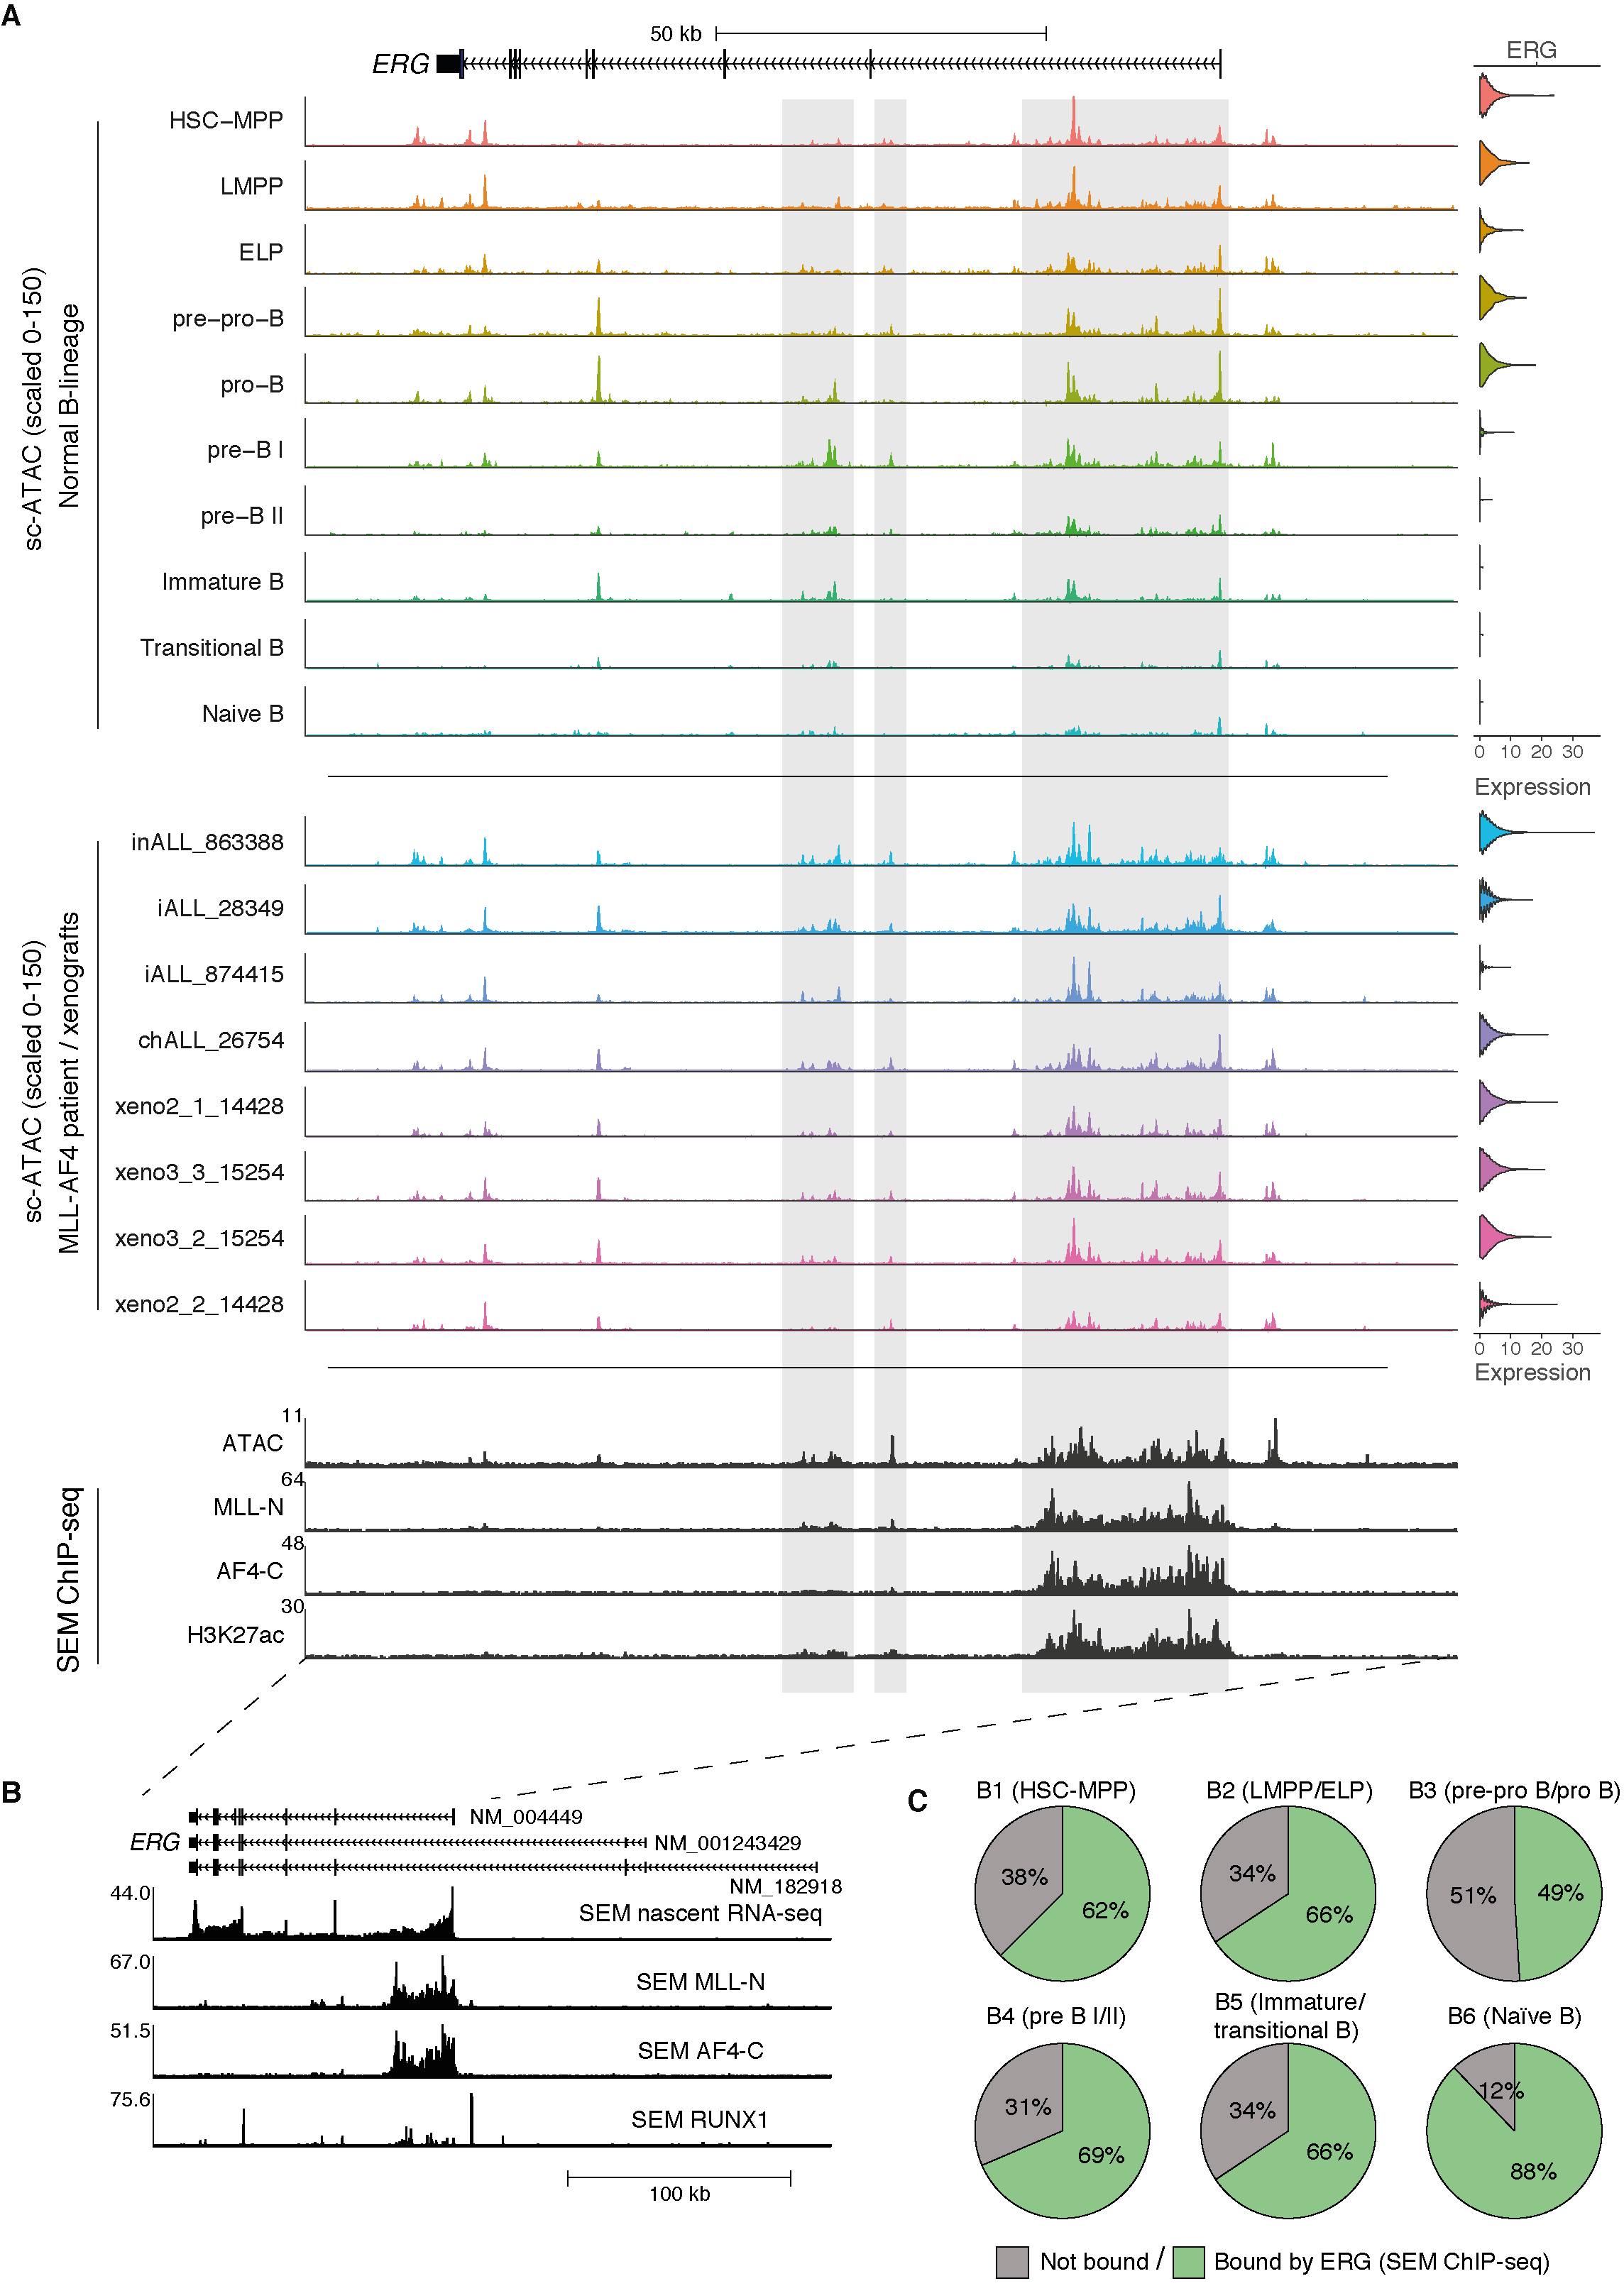
\includegraphics[width=\textwidth,height=\textheight,keepaspectratio]{figures/chapter4/ch4_multiome-erg.png}
    \caption[{MLL-AF4 and RUNX1 regulate a specific isoform of the fetal B-progenitor TF, \textit{ERG}.}]
    {\textbf{MLL-AF4 and RUNX1 regulate a specific isoform of the fetal B-progenitor TF, \textit{ERG}.} 
    \textit{Legend continued on next page.}
    %\textbf{(A)} Panel of ATAC-seq and ChIP-seq tracks at the \textit{ERG} locus. scATAC-seq tracks are pseudobulked by cluster identity (FL/FBM) or sample identity (ALL blasts). Bulk ATAC-seq and ChIP-seq from SEM cells shown at the bottom. \textit{ERG} expression shown on the right.
    %\textbf{(B)} Zoomed out tracks showing three \textit{ERG} isoforms, and SEM nascent RNA-seq and ChIP-seq.
    %\textbf{(C)} Proportion of B lymphopoiesis signatures bound by ERG ChIP-seq.
    }
    \label{fig:ch4_multiome-erg}
\end{figure}

One factor of interest is \textit{ERG}, expressed in an ELP/LMPP biased signature (B2), which is expressed until pro-B and downregulated in pre-B cells. Pseudo-bulked accessibility profiles of the \textit{ERG} locus in ALL blasts match pre-pro-B and pro-B cells, and the gene is bound by spreading MLL-AF4 and RUNX1 in SEM cells. This suggests MLL-AF4 and cooperative TFs bind to the accessible landscape in pro-B cells and prevents inactivation of the locus (Fig. \ref{fig:ch4_multiome-erg}A). There are two \textit{ERG} transcripts commonly expressed in haematopoietic cells, \textit{ERG2} (NM\_004449) and \textit{ERG3} (NM\_182918) \citep{bohne_epigenetic_2009}. Interestingly, MLL-AF4 and RUNX1 are only bound at the TSS of the \textit{ERG2} transcript, and only \textit{ERG2} transcripts are expressed (Fig. \ref{fig:ch4_multiome-erg}B), suggesting the MLL-AF4 drives a shift in \textit{ERG} isoforms, though the consequence of this is not clear. \textit{ERG} expression is required for V-to-DJ recombination and progression from a pro-B to pre-B state \citep{sondergaard_erg_2019}, yet \textit{ERG} overexpression in mouse haematopoiesis also results in an expansion of pro-B cells and a partial pro-B to pre-B block \citep{tsuzuki_promotion_2011}. As such, ERG may be required for V-to-DJ recombination but must be downregulated thereafter, hence forced expression could contribute to an ALL B differentiation block. In fact, ERG ChIP-seq shows binding at a higher proportion of the Na\"{i}ve B signature (B6) genes compared to other signatures (Fig. \ref{fig:ch4_multiome-erg}C), suggesting downstream ERG interaction with mature B programs. Altogether, these analyses highlight the capacity for MLL-AF4, and cooperating TFs, to drive normal fetal circuits, reactivate stem and progenitor TFs, and potentially to repress mature B-cell programs, leading to a block in differentiation.
\begin{figure}[!t]
    \ContinuedFloat
    \hrule
    \vspace{5mm}
    \caption[]
    {\textit{Legend continued from previous page}. 
    \textbf{(A)} Panel of ATAC-seq and ChIP-seq tracks at the \textit{ERG} locus. scATAC-seq tracks are pseudobulked by cluster identity (FL/FBM) or sample identity (ALL blasts). Bulk ATAC-seq and ChIP-seq from SEM cells shown at the bottom. \textit{ERG} expression shown on the right.
    \textbf{(B)} Zoomed out tracks showing three \textit{ERG} isoforms, and SEM nascent RNA-seq and ChIP-seq.
    \textbf{(C)} Proportion of B lymphopoiesis signatures bound by ERG, based on ChIP-seq peaks. 
    \textit{ERG ChIP-seq data was sourced \citep{godfrey_dot1l_2019}.}
    }
\end{figure}
\vspace*{3in}


\clearpage
\section{Conclusions and discussion}

The central hypothesis of this chapter, based on the observation that \textit{MLL-AF4} KD results in gene expression changes disconnected from direct MLL-AF4 binding, is that activated TFs are an essential component of \textit{MLL}r networks. MLL-AF4 overexpresses a number of highly connected TFs, which may directly cooperate with MLL-AF4 to modulate gene expression, or act as an intermediate factor to regulate a wider network. To ask what the role of these activated TFs are in the wider MLL-AF4 network, I established GRN models describing the regulatory logic of MLL-AF4, the primary driver of leukaemic transformation \citep{andersson_landscape_2015, bardini_dna_2010, bardini_implementation_2011}, and RUNX1, a critical central TF. 

By integrating the MLL-AF4 GRN with patient expression data, I was able to organise nodes into modules (section \ref{ch4:patient-modules}, Fig. \ref{fig:ch4_patient}). This identified a number of B progenitor nodes that are either maintained or overexpressed in ALL blasts (Patient module 1-3), as well as a number of genes that are uniquely activated in leukaemia (Patient module 4). This was an early suggestion that the MLL-AF4 network co-opts B progenitor circuits. This analysis also identified a cell line specific module (Patient module 5), which reflects an immortalised cell line phenotype. This module is unsurprising, considering the extensive transcriptional adaptations that occur in cell lines \citep{lopes-ramos_regulatory_2017}, but highlights a problem with performing network analyses in cell line models. Perturbation studies are not feasible in donor patient samples, but cell line specific nodes can be removed through this integration with patient expression data. The most interesting observation was that many modules showed commonality across both AML and ALL samples (Patient modules 1, 2, 4), and that these were enriched for highly central TFs (section \ref{ch4:patient-core}, Fig. \ref{fig:ch4_core}). This analysis suggested the existence of a core network across both AML and ALL, and further validation in THP-1 cells confirmed common network interactions between MLL-AF4 and MLL-AF9 fusion proteins. This is an exciting observation, as this central network may anchor MLL-AF4 behaviour in both myeloid and lymphoid lineages and explain how \textit{MLL}r leukaemias can undergo lineage switching \citep{dorantes-acosta_lineage_2012, gardner_acquisition_2016}. While MLL-FP regulates similar central TFs across AML and ALL, the same is not true for RUNX1, which demonstrates context-specific differences. This leads to an interesting possibility, where MLL-AF4 activates a common panel of TFs, but these TFs can enact context-specific regulation.

Centrality analysis of the MLL-AF4 GRN, using degree and stress centralities, highlighted a number of interesting TFs (section \ref{ch4:stress-centrality}). An important metric is the ratio of degree (connectivity) and stress centralities, which has been suggested to represent key nodes connecting distinct network modules \citep{joy_high-betweenness_2005, koschutzki_centrality_2008}. As such, we can infer that a high degree/stress ratio represents network paths with low robustness that may be susceptible to perturbation. RUNX1 and MYB are two TFs with a very high degree/stress ratio, and are both critically essential in MLL-AF4 and MLL-AF9 leukaemias. Additional central factors include ELF1, MAZ, MYC and NF-YA, among others. MAZ, despite high connectivity, had a low degree/stress ratio which was reflected in a lack of essentiality across multiple CRISPR screens. Despite this, MAZ was revealed to be a significant activator of \textit{MYC}, in line with its discovery as a \textit{MYC} associated zinc finger \citep{komatsu_maz_1997}, and to a lesser degree \textit{BCL2}. NF-YA is a particularly interesting, and little explored target of MLL-AF4. By essentiality screens \textit{NFYA} perturbation had little overall effect, and like MAZ it had a poor degree/stress ratio. Despite this, \textit{MLL}r cell lines had overall greater essentiality scores for \textit{NFYA} targeting in the DepMap database over non-\textit{MLL}r blood cancers. A recent pre-print study has suggested a novel role in leukaemia, where NF-YA associates with, and directs the binding of Menin \citep{soto-feliciano_molecular_2022}. As Menin is a key MLL-FP complex component, this may direct binding of MLL-AF4 to non-uCpG sites. Other central factors of note were CEBPA and MED13L, which were not only highly connected, but showed much higher essentiality in \textit{MLL}r leukaemias over non-\textit{MLL}r. CEBPA also held a very high degree/stress ratio. CEBPA is commonly mutated in AML and thought to be involved in \textit{MLL}r leukaemia initiation \citep{roe_cebp_2014}. By contrast, MED13L has had little study in leukaemia, positioning it as a novel essential protein specific to \textit{MLL}r cancers. The mediator complex, of which MED13L is a subunit of, acts as an intermediate complex associating TF binding with pol II activity, stabilises enhancer-promoter loops, and is a characteristic of super enhancers \citep{allen_mediator_2015, whyte_master_2013}. MLL-AF4 spreading is associated with MED1 \citep{kerry_mll-af4_2017}, and MED26 interacts components of the SEC \citep{takahashi_human_2011}, suggesting a significant interplay between MLL-FP and the mediator complex in regulating transcription.

\begin{figure}[!t]
    \centering
    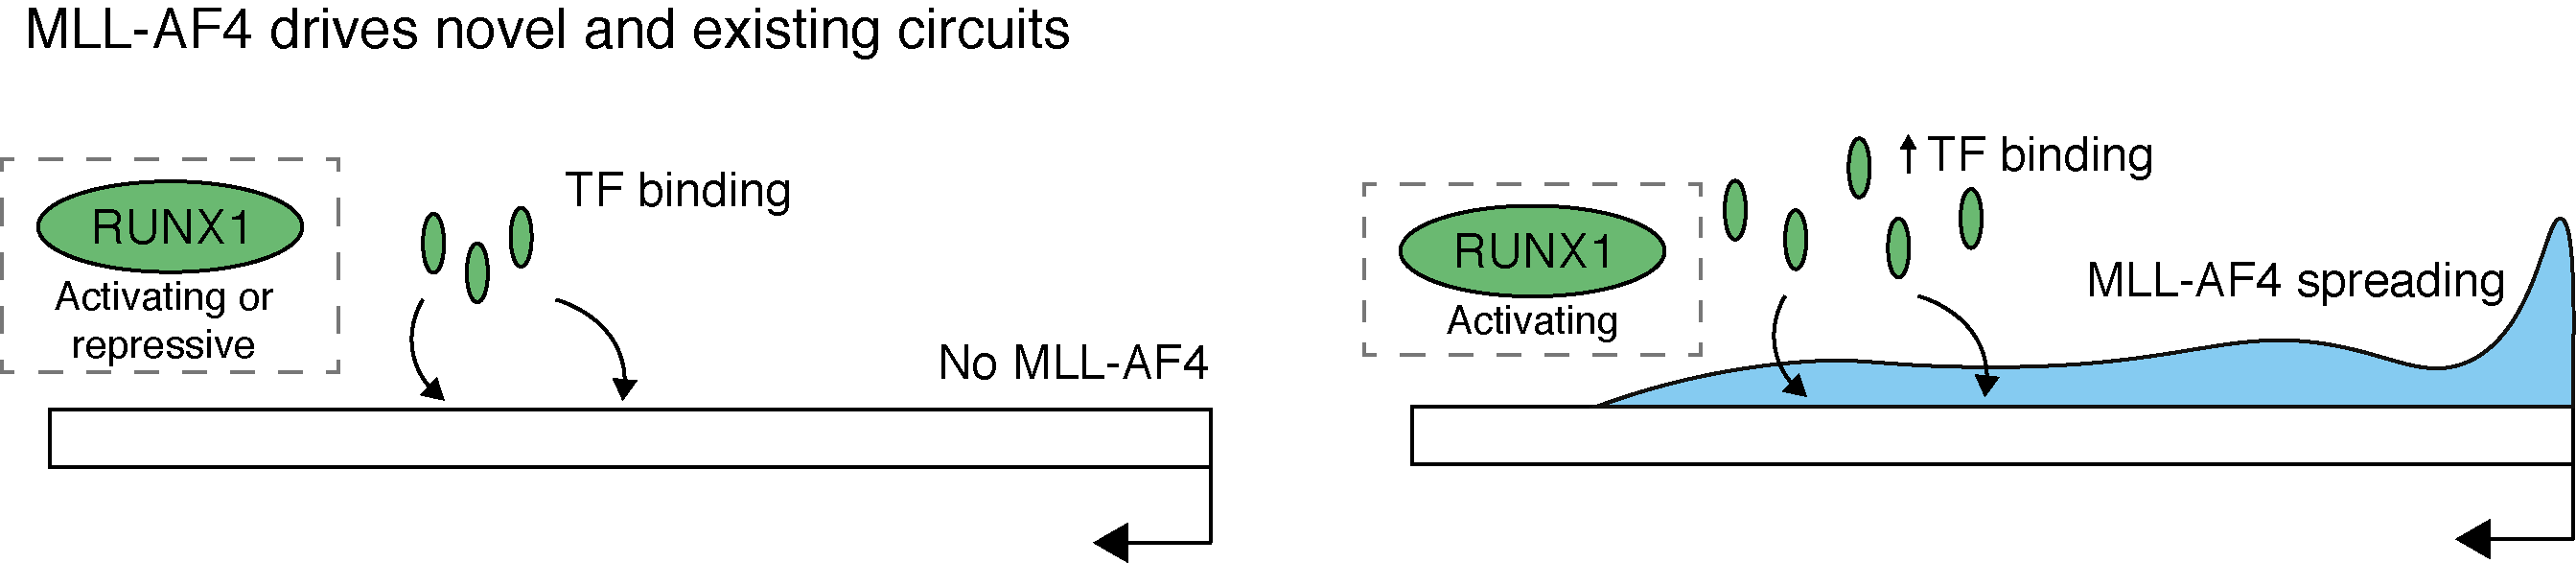
\includegraphics[width=\textwidth,keepaspectratio]{figures/models/ch4_model-ma4-novel.png}
    \caption[{Summary model of how MLL-AF4 binding may alter TF activity.}]
    {\textbf{Summary model of how MLL-AF4 binding may alter TF activity.}
    A model illustrating how MLL-AF4 binding may alter TF activity within the GRN model. MLL-AF4 spreading was shown to be associated with an increased frequency of TF peaks, which is most likely driven through increased affinity for DNA binding motifs. This increased affinity synergises with MLL-AF4, by encouraging binding of TFs, and may allow for novel regulatory interactions. Further, RUNX1 activity at non-MLL-AF4 sites shows activation and repression, whereas at MLL-AF4 bound genes it is biased towards activation.
    }
    \label{fig:ch4_model-ma4-novel}
\end{figure}

Taking RUNX1 as an example central TF, my analysis led to a thorough investigation of the interplay between MLL-AF4 and RUNX1 (section \ref{ch4:ma4-runx1}). The role of TFs in the MLL-AF4 network can be broadly categorised into two types: TFs acting as an intermediate regulatory factor, as in the case of TF cascades, or through TF cooperativity forming FFL circuits. As such, MLL-AF4 and RUNX1 regulatory logic was organised into FFL and cascade motifs, and used to explore how MLL-AF4 could impact transcription beyond its direct binding to chromatin. This highlighted a number of MLL-AF4:RUNX1 driven cascade motifs, including an MLL-AF4:RUNX1:\textit{CASP9} repressive chain that may promote cell survival. Interestingly, there were a large number of MLL-AF4:RUNX1 driven FFL motifs, and while RUNX1 can both activate and repress target genes (as seen with cascade motifs), in the context of MLL-AF4 binding RUNX1 regulatory logic is instead biased towards activation. It was also found that MLL-AF4 binding across chromatin was correlated with RUNX1 (section \ref{ch4:ma4-runx1-cor}, Fig. \ref{fig:ch4_ma4-TF-cor}), and appeared to promote TF:DNA binding affinity. Together, this strongly suggests that MLL-AF4 co-opts overexpressed TFs to further drive gene expression by cooperative regulation, and may promote the establishment of novel GRN interactions by encouraging the binding of TFs to DNA binding motifs (Fig. \ref{fig:ch4_model-ma4-novel}). MLL-AF4 also appears to alter TF activities, as seen where RUNX1 is biased towards activation at MLL-AF4 targets (Fig. \ref{fig:ch4_model-ma4-novel}). This TF cooperation was exemplified at \textit{BCL2} and \textit{MYC} where RUNX1 cooperates with MYB, in the context of MLL-AF4 binding, to enhance activation of these genes, leading to increased cell survival and proliferation (section \ref{ch4:tf-cointeraction}, Fig. \ref{fig:ch4_model-ma4-myc-bcl2}). 

\begin{figure}[htbp]
    \centering
    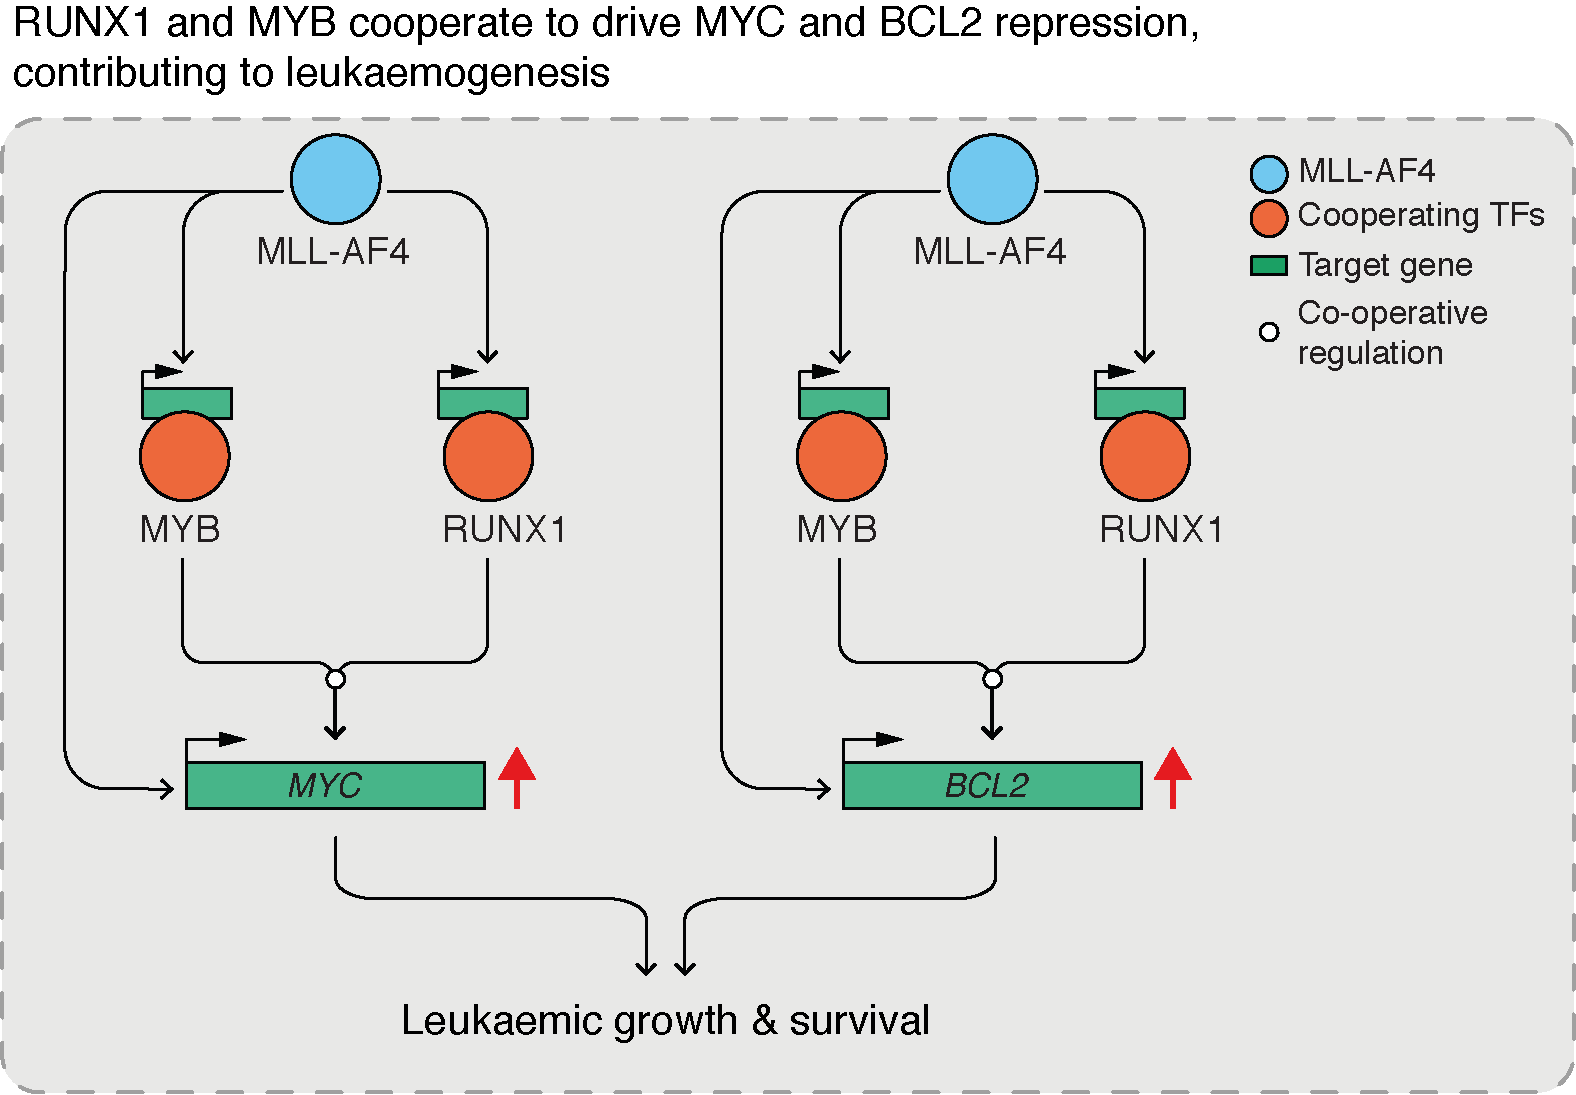
\includegraphics[width=\textwidth,keepaspectratio]{figures/models/ch4_model-ma4-myc-bcl2.png}
    \caption[{Summary model of RUNX1 and MYB cooperation to drive \textit{MYC} and \textit{BCL2} expression.}]
    {\textbf{Summary model of RUNX1 and MYB cooperation to drive \textit{MYC} and \textit{BCL2} expression.}
    A model of MLL-AF4-driven regulation of \textit{MYC} and \textit{BCL2}. RUNX1 and MYB cooperate to drive gene expression of both \textit{MYC} and \textit{BCL2}, which are known to functionally cooperate to drive leukaemic growth and survival \citep{fanidi_cooperative_1992, bissonnette_apoptotic_1992}. 
    \textit{Figure is adapted from \cite{harman_kmt2a-aff1_2021}}. 
    }
    \label{fig:ch4_model-ma4-myc-bcl2}
\end{figure}

It was also noted that the MLL-AF4 network may maintain, or overexpress fetal circuits. Applying the MLL-AF4 GRN to B progenitor expression signatures highlighted significant interactions throughout B lymphopoiesis (section \ref{ch4:multiome}). In particular, the MLL-AF4 GRN appears to strongly activate a pre-pro-B/pro-B signature and repress stem and mature B-cell signatures. However, several TFs preferentially expressed in HSCs were regulated by MLL-AF4 in cooperation with RUNX1, including \textit{HMGA2} and \textit{ANGPT1}, which suggests a reactivation of HSC pathways (Fig. \ref{fig:ch4_model-ma4-coopt}). \textit{HMGA2} is a known target of MLL-AF4 that promotes leukaemic growth \citep{eguchi-ishimae_hmga2_2014, guenther_aberrant_2008}, and has a role in genome wide remodelling of chromatin accessibility at AT rich sites \citep{vignali_hmga_2020}. \textit{HMGA2} by our analysis is typically downregulated as cells differentiate, and this maintained expression likely promotes global gene expression. \textit{ANGPT1} (Angiopoietin-1) is also biased towards HSCs, where Angiopoietin-1 is secreted by HSCs to maintain their vascular niche in bone marrow \citep{zhou_hematopoietic_2015}. \textit{ANGPT1} was previously found to be regulated by MLL-AF4 in SEM cells \citep{castro_angiopoietin1_2010}, where it was noted that \textit{ANGPT1} perturbation resulted in cell cycle arrest and reduced splenic infiltration in transplantation experiments. This highlights the utility of this analysis for identifying reactivation of early stem cell circuits in MLL-AF4 leukaemia, though the additional role of RUNX1 in regulating these targets in leukaemia has not previously been explored. \textit{ERG} is a specific MLL-AF4:RUNX1 target highly regulated by MLL-AF4, that is normally expressed up to pro-B cells before repression in pre-B cells (Fig. \ref{fig:ch4_model-ma4-coopt}). \textit{ERG} is critical for V-to-DJ recombination, and promotes pro-B to pre-B differentiation \citep{sondergaard_erg_2019}, but this is incongruous with mouse experiments noting an expansion of pro-B cells and a partial pro-B to pre-B block with \textit{ERG} overexpression \citep{tsuzuki_promotion_2011}. One hypothesis that explains this is that ERG may be required for V-to-DJ recombination but must be downregulated thereafter for B progenitor differentiation. Therefore, forced expression by MLL-AF4 may contribute to an ALL B differentiation block (Fig. \ref{fig:ch4_model-ma4-coopt}), though further study is required to determine the validity of this hypothesis. 

\begin{figure}[htbp]
    \centering
    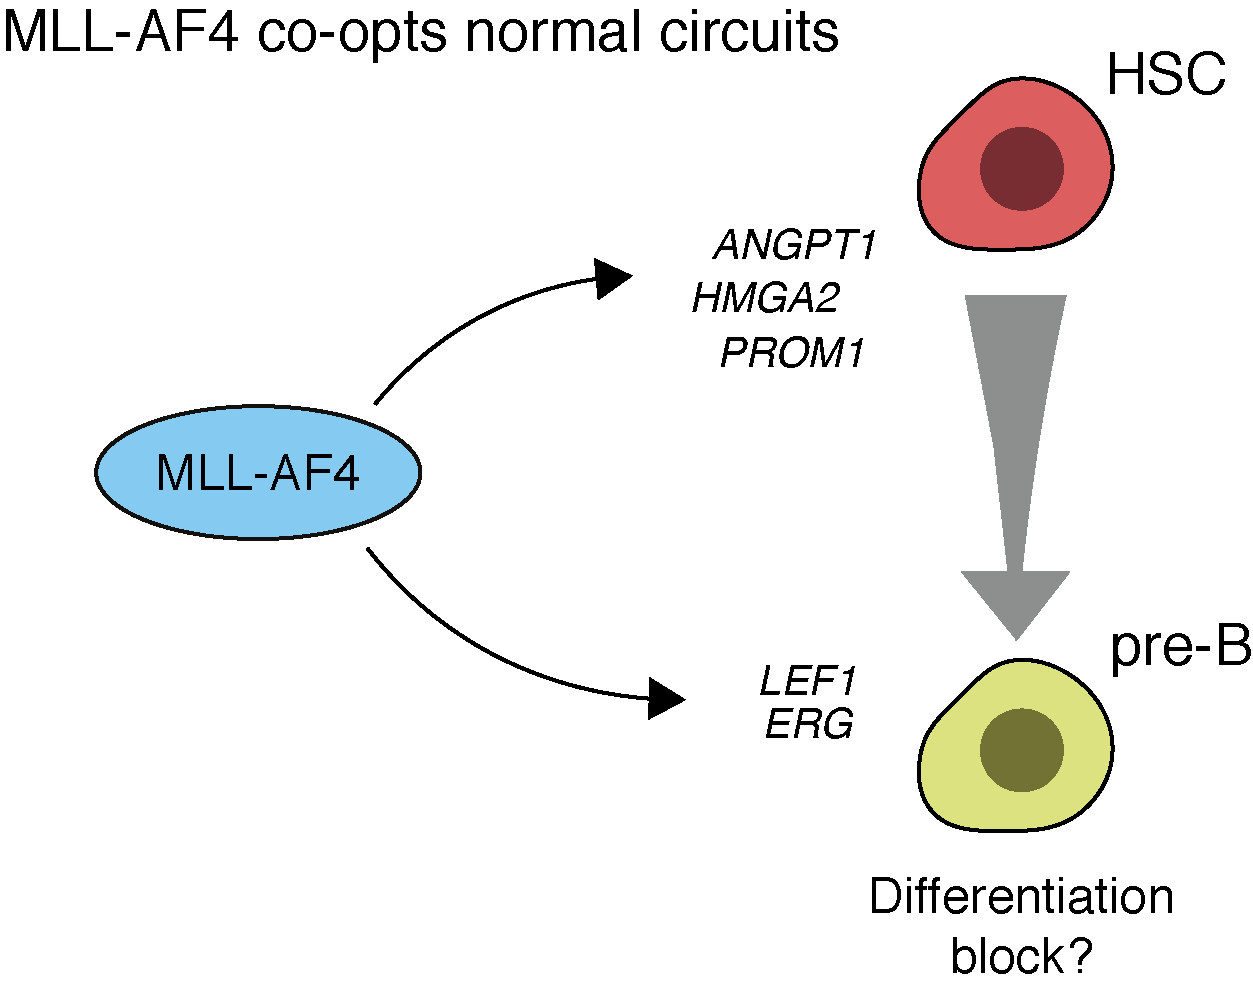
\includegraphics[width=0.5\textwidth,height=\textheight,keepaspectratio]{figures/models/ch4_model-ma4-coopt.png}
    \caption[{Summary model describing MLL-AF4 activation of developmental circuits.}]
    {\textbf{Summary model describing MLL-AF4 activation of developmental circuits.}
    A model illustrating MLL-AF4 reactivation of early HSC-expressing genes, or maintenance of genes expressed in pro-B or pre-B cells. In doing so, MLL-AF4 can be considered to co-opt and force maintained activation of these circuits, which may contribute to the block in \textit{MLL}r ALL differentiation.
    }
    \label{fig:ch4_model-ma4-coopt}
\end{figure}
